\section{Menschliche und tierische Proben unter dem Mikroskop}

\newpage
\subsection{Menschlicher Dünndarm}

\subsubsection{Proben}
\begin{table}[h!]
	\centering
	\begin{tabular}{l l}
		Bezeichnung	& Mammal Ileum \\
		Probe 		& 31-5226
	\end{tabular}
\end{table}

\subsubsection{Aufzeichnungen}
\begin{figure}[h!]
	\centering
	\begin{subfigure}[b]{0.3\textwidth}
		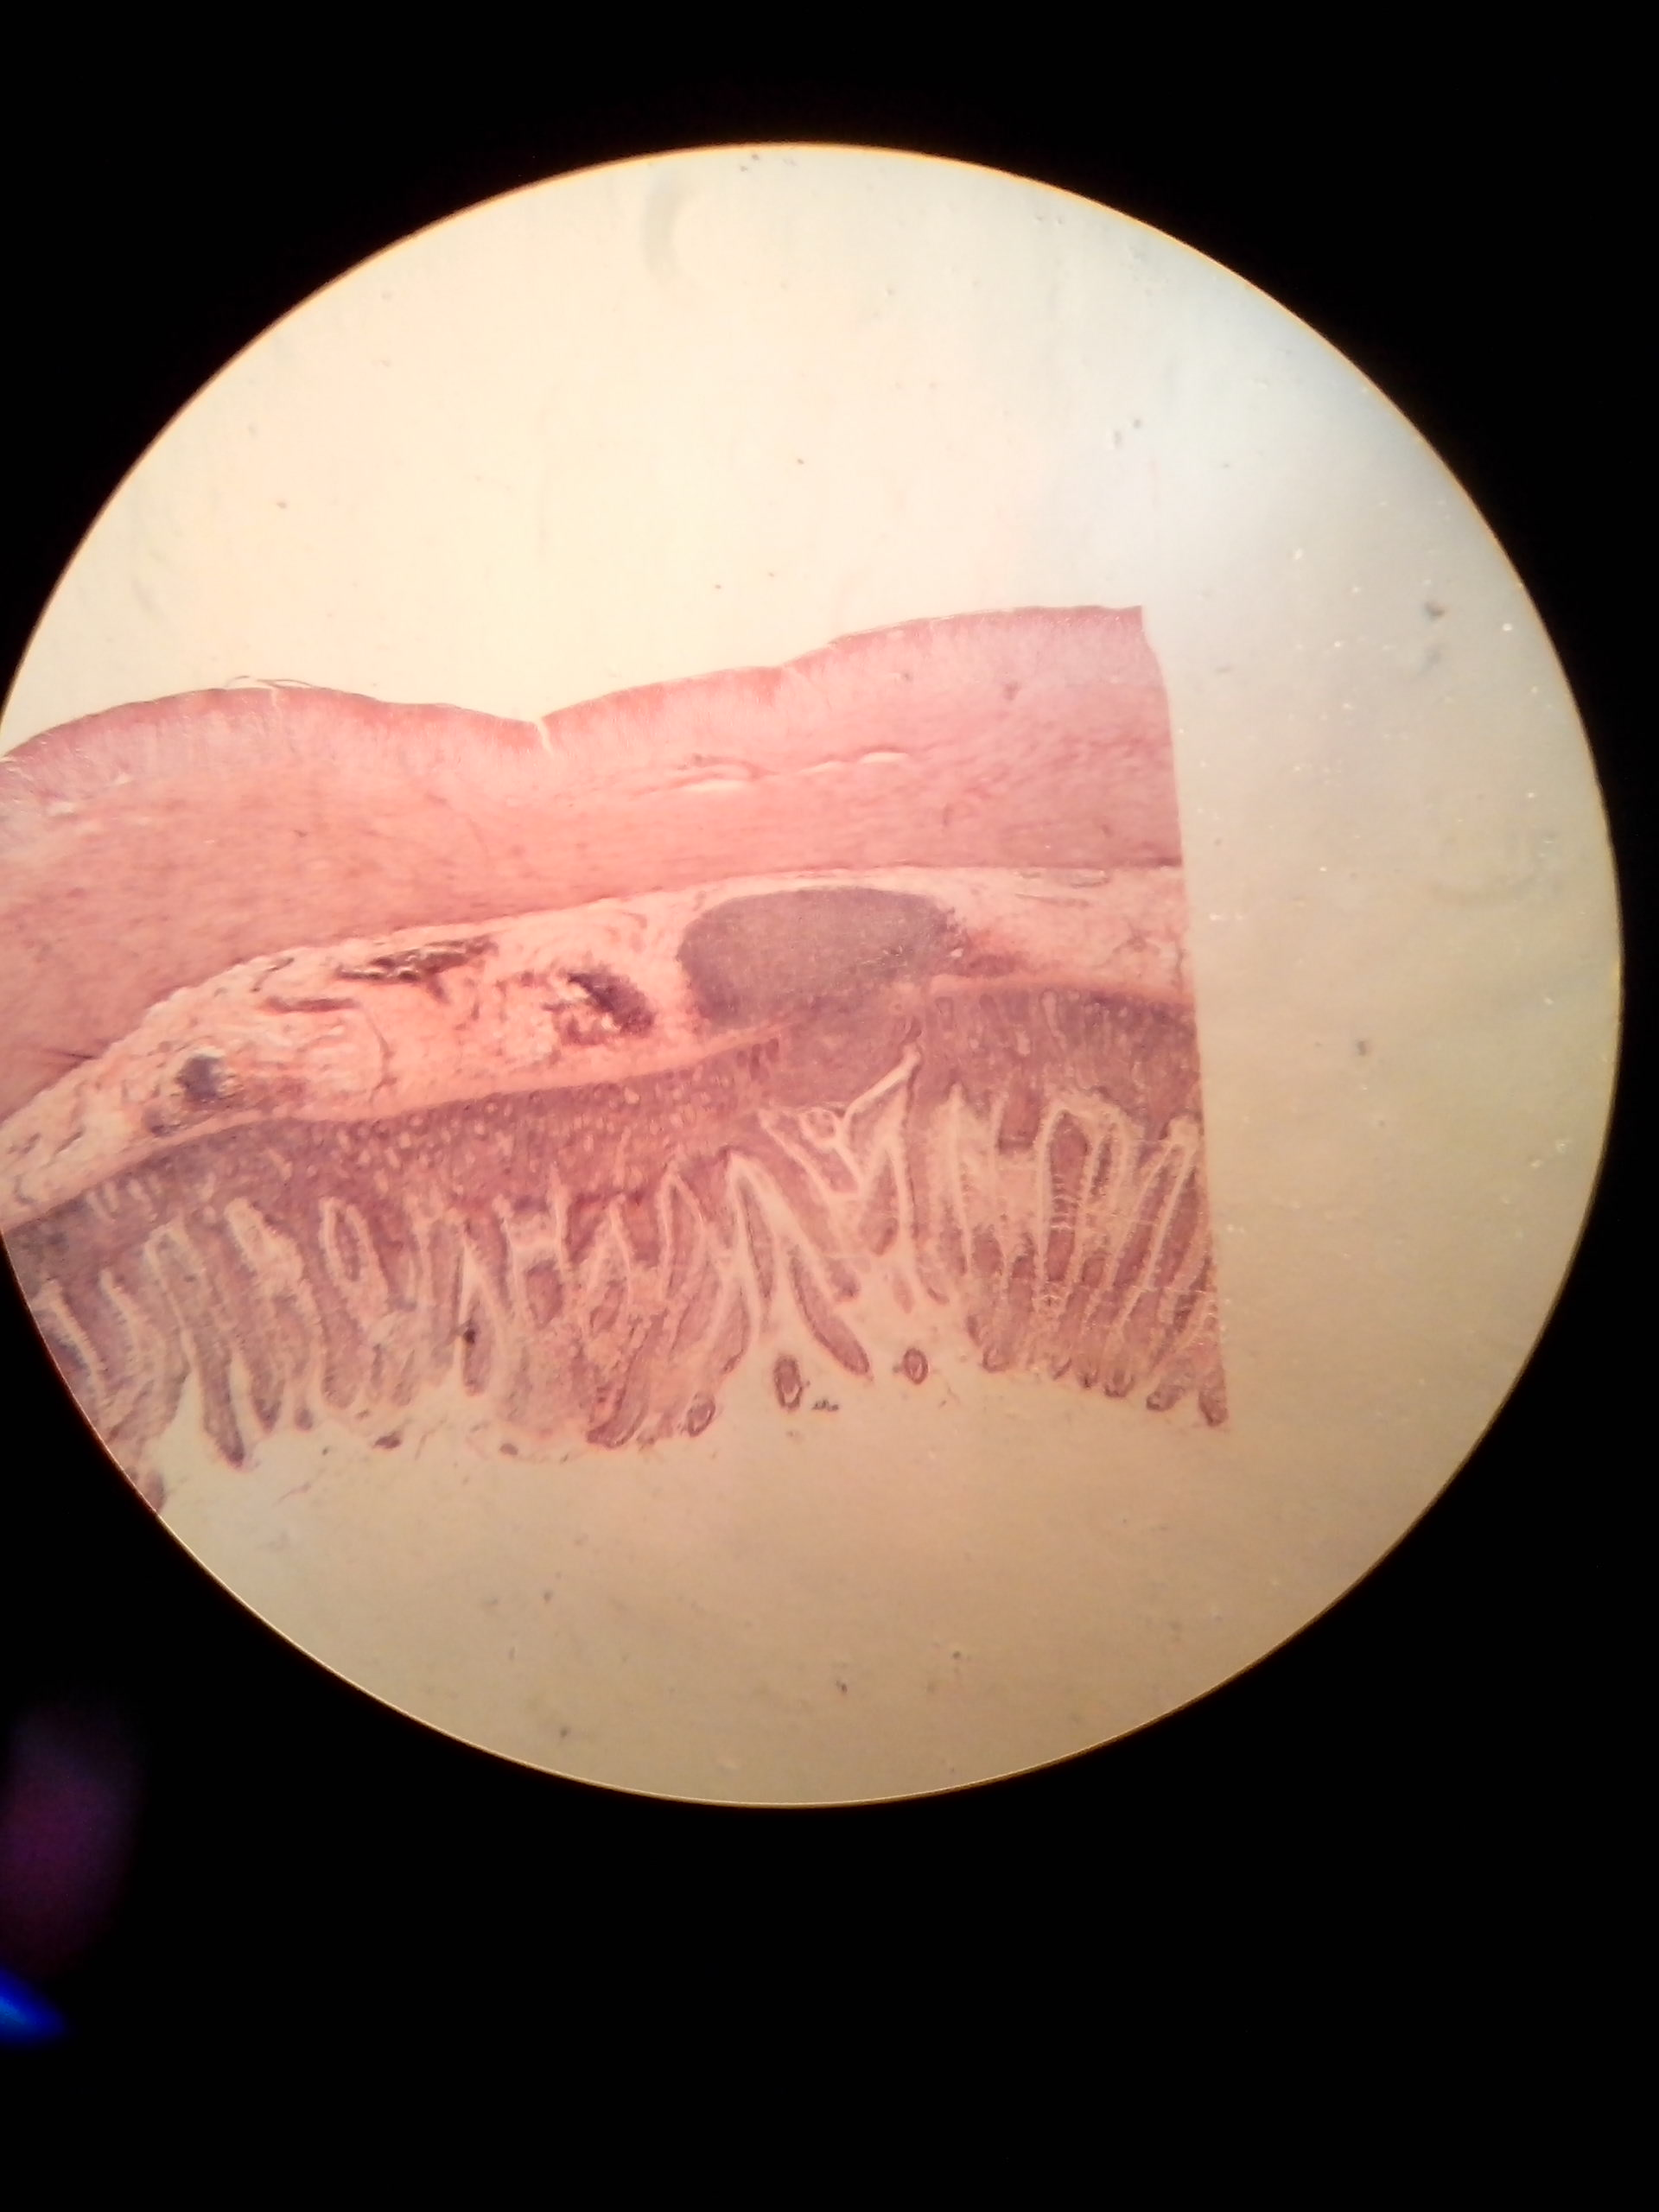
\includegraphics[width=1\textwidth]{../images/01_mammal_illeum.jpg}
		\caption{Objektiv 4x}
		\label{fig:01_mammal_ileum}
	\end{subfigure}
	\begin{subfigure}[b]{0.3\textwidth}
		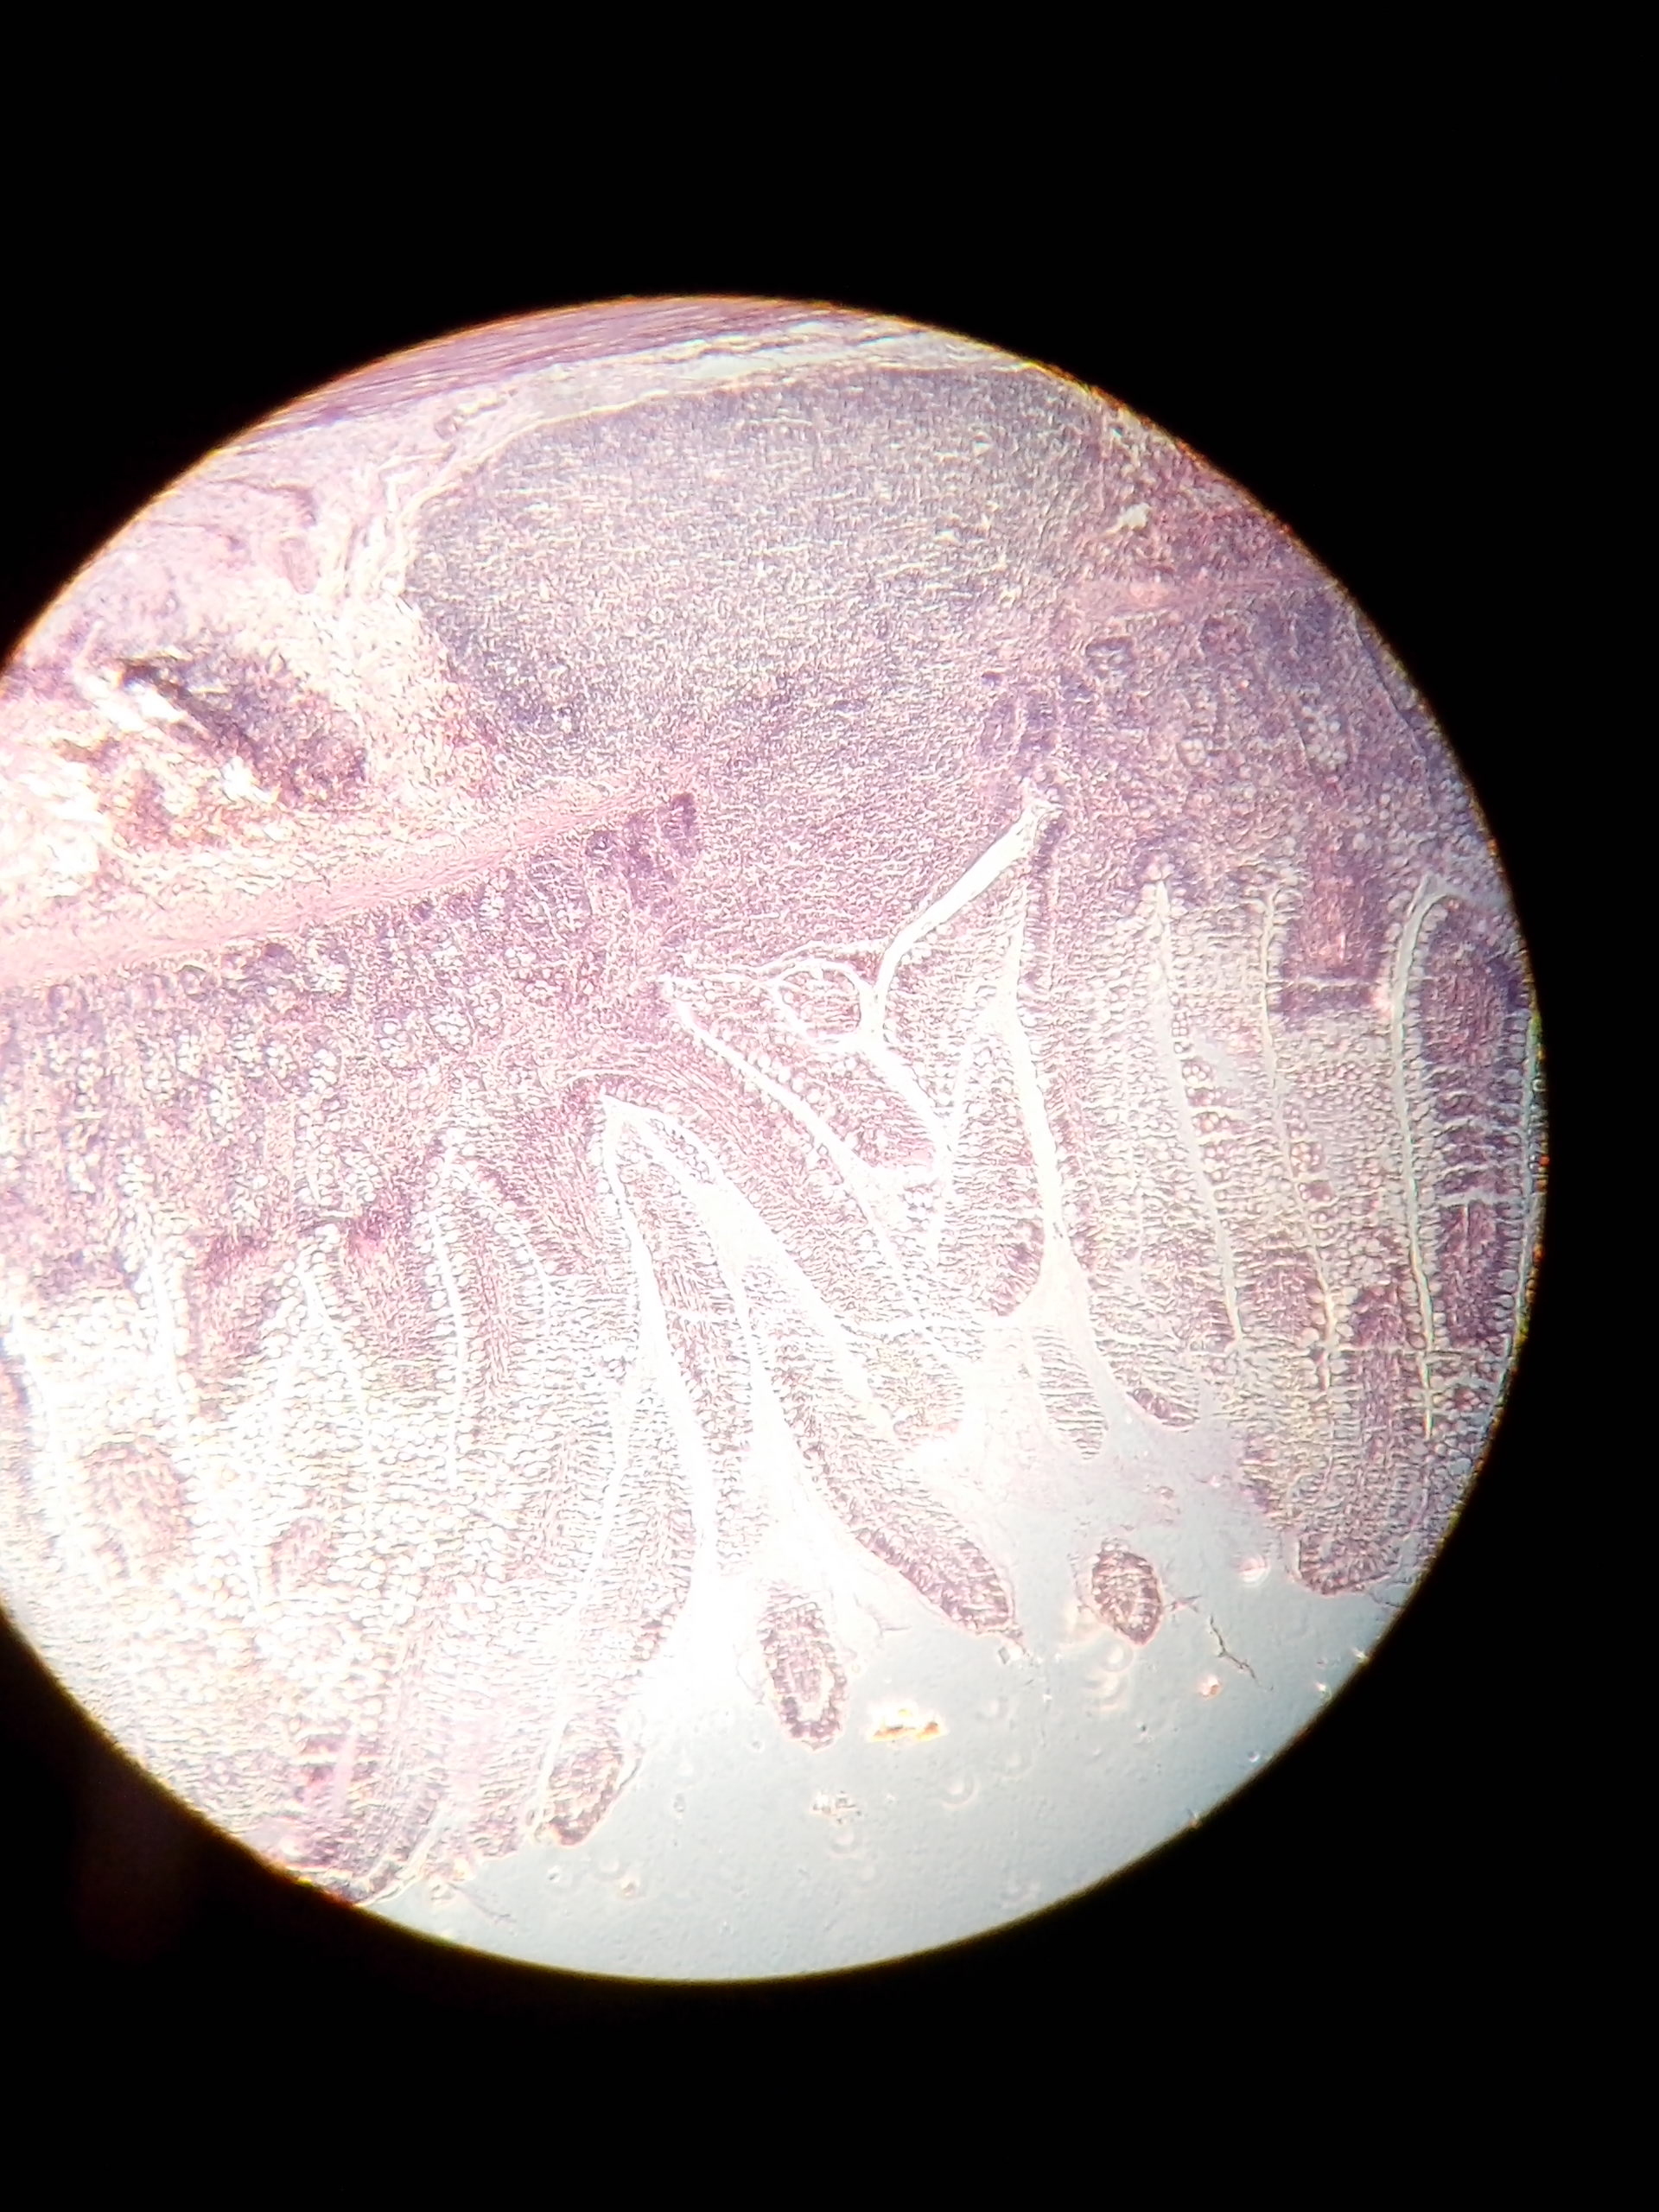
\includegraphics[width=1\textwidth]{../images/02_mammal_illeum.jpg}
		\caption{Objektiv 10x}
		\label{fig:02_mammal_ileum}
	\end{subfigure}
	\begin{subfigure}[b]{0.3\textwidth}
		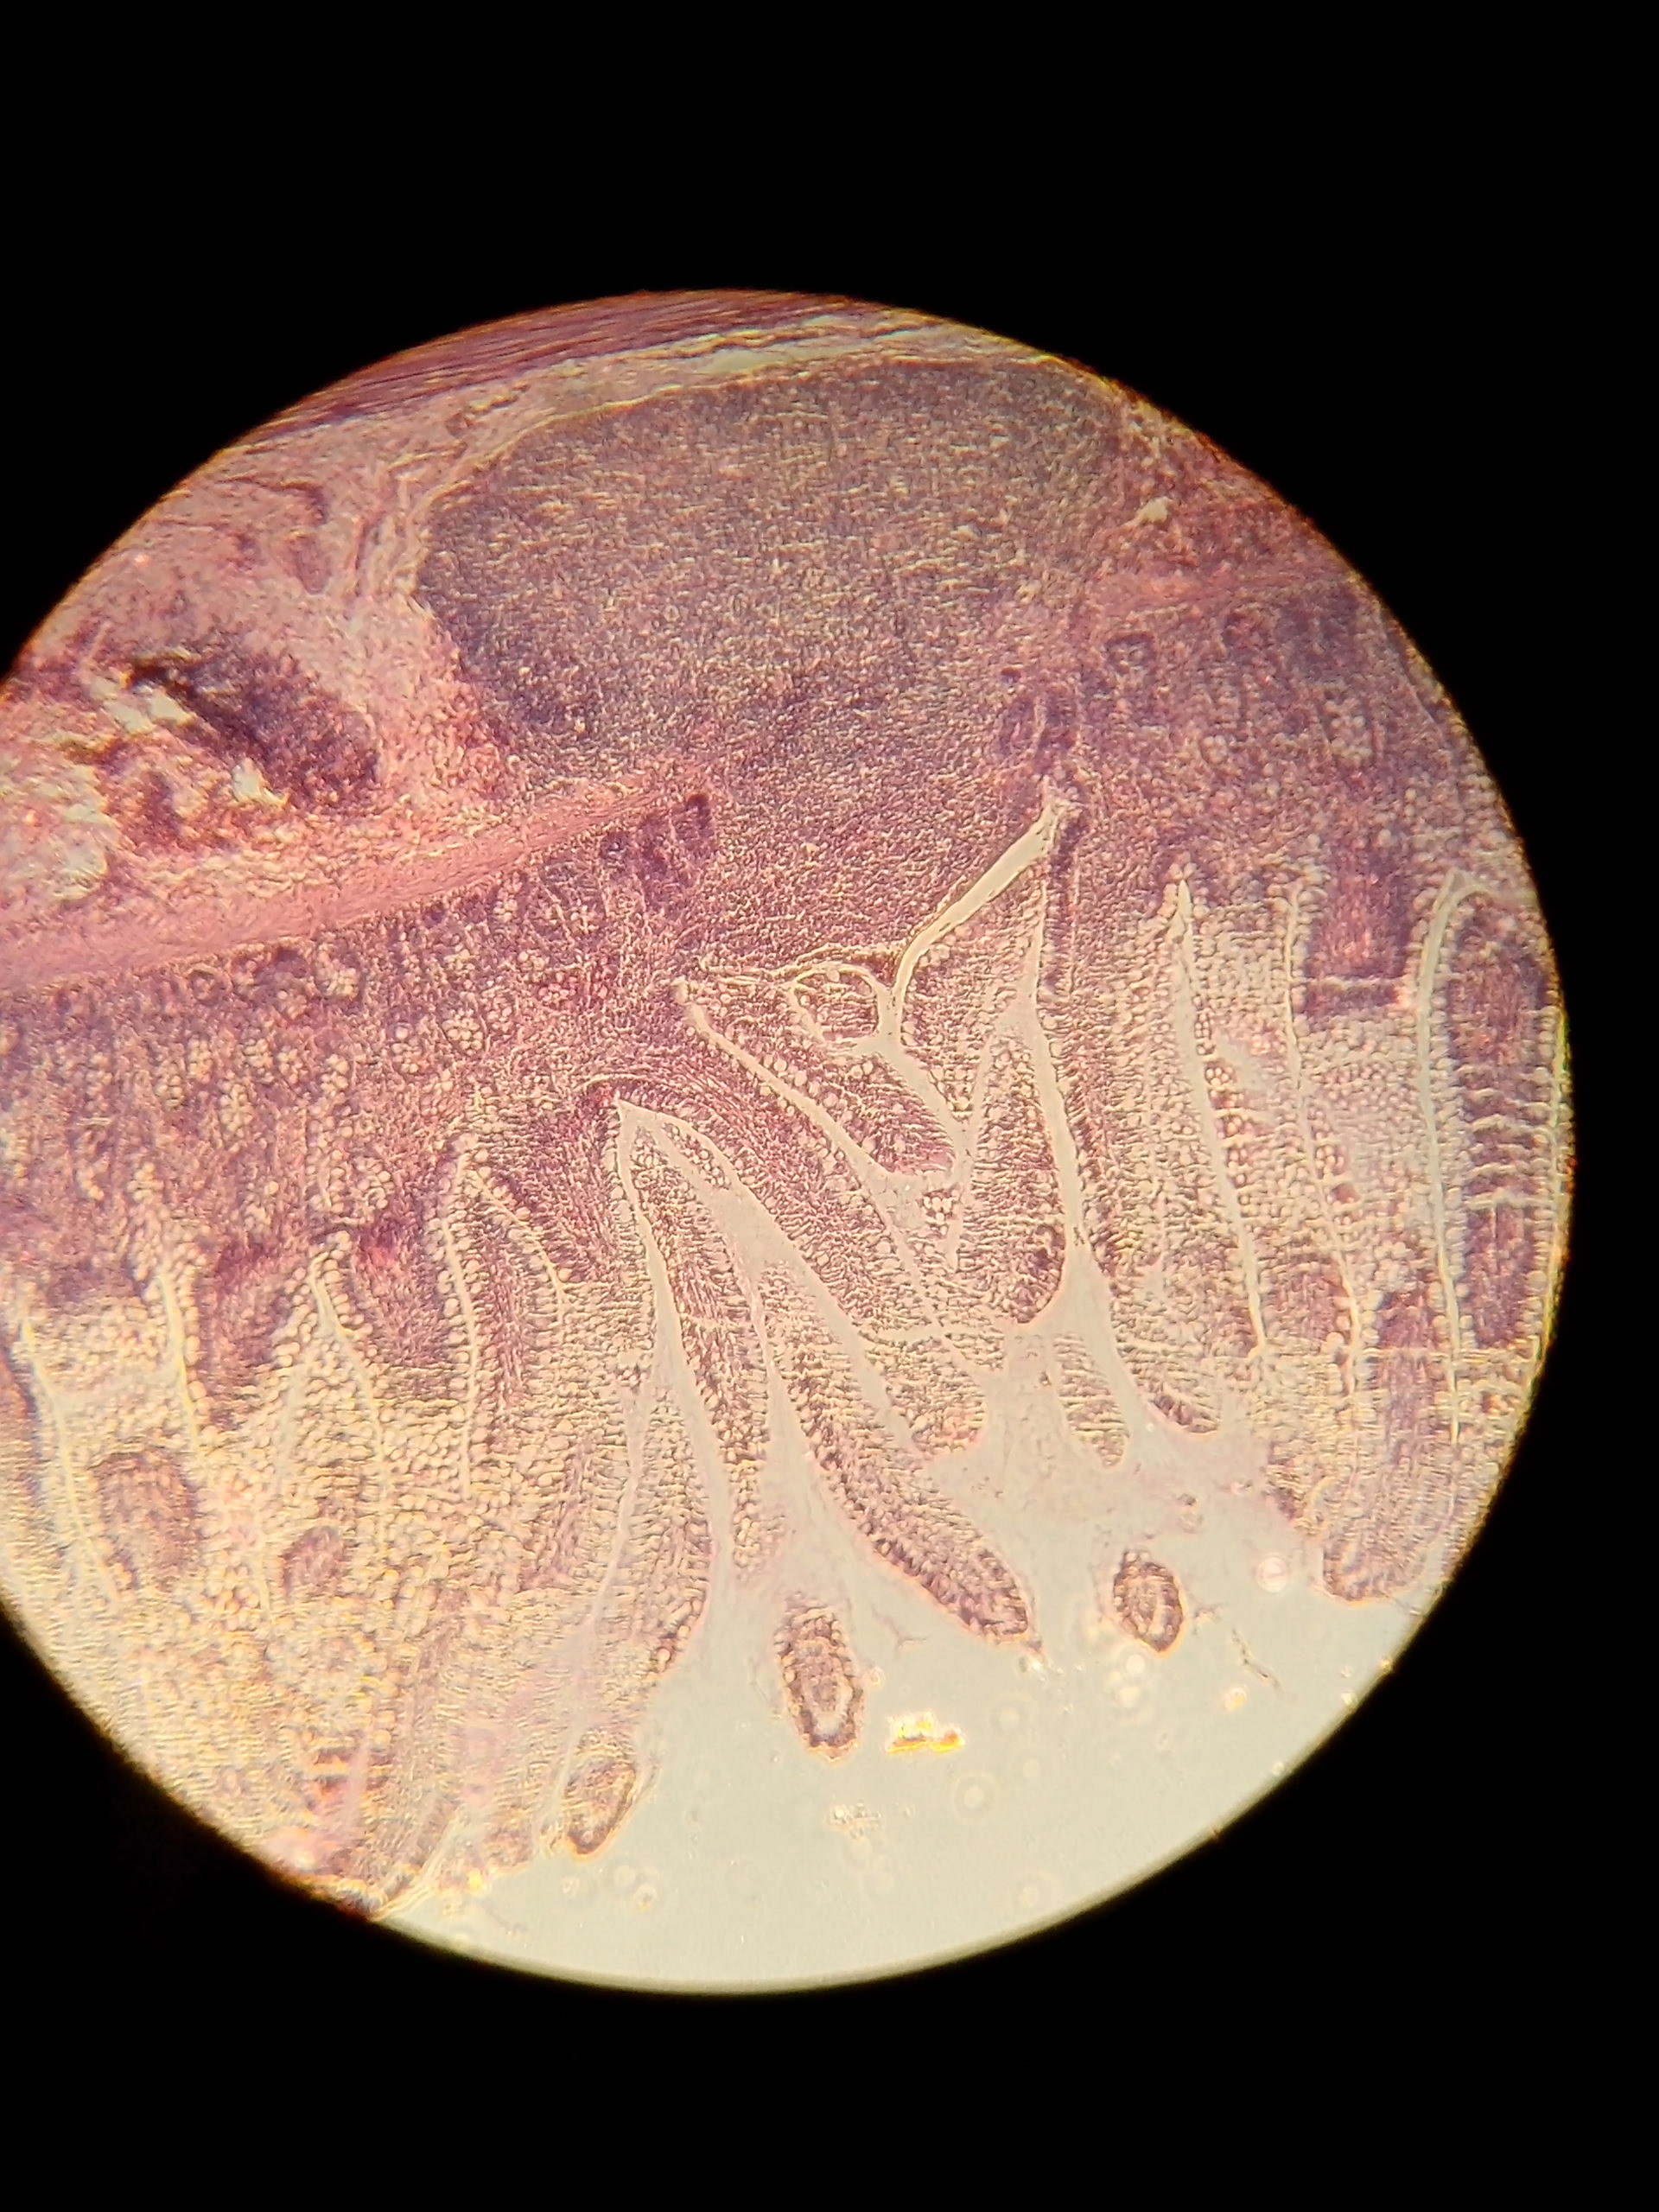
\includegraphics[width=1\textwidth]{../images/03_mammal_illeum.jpg}
		\caption{Objektiv 10x}
		\label{fig:03_mammal_ileum}
	\end{subfigure}

	\begin{subfigure}[b]{0.3\textwidth}
		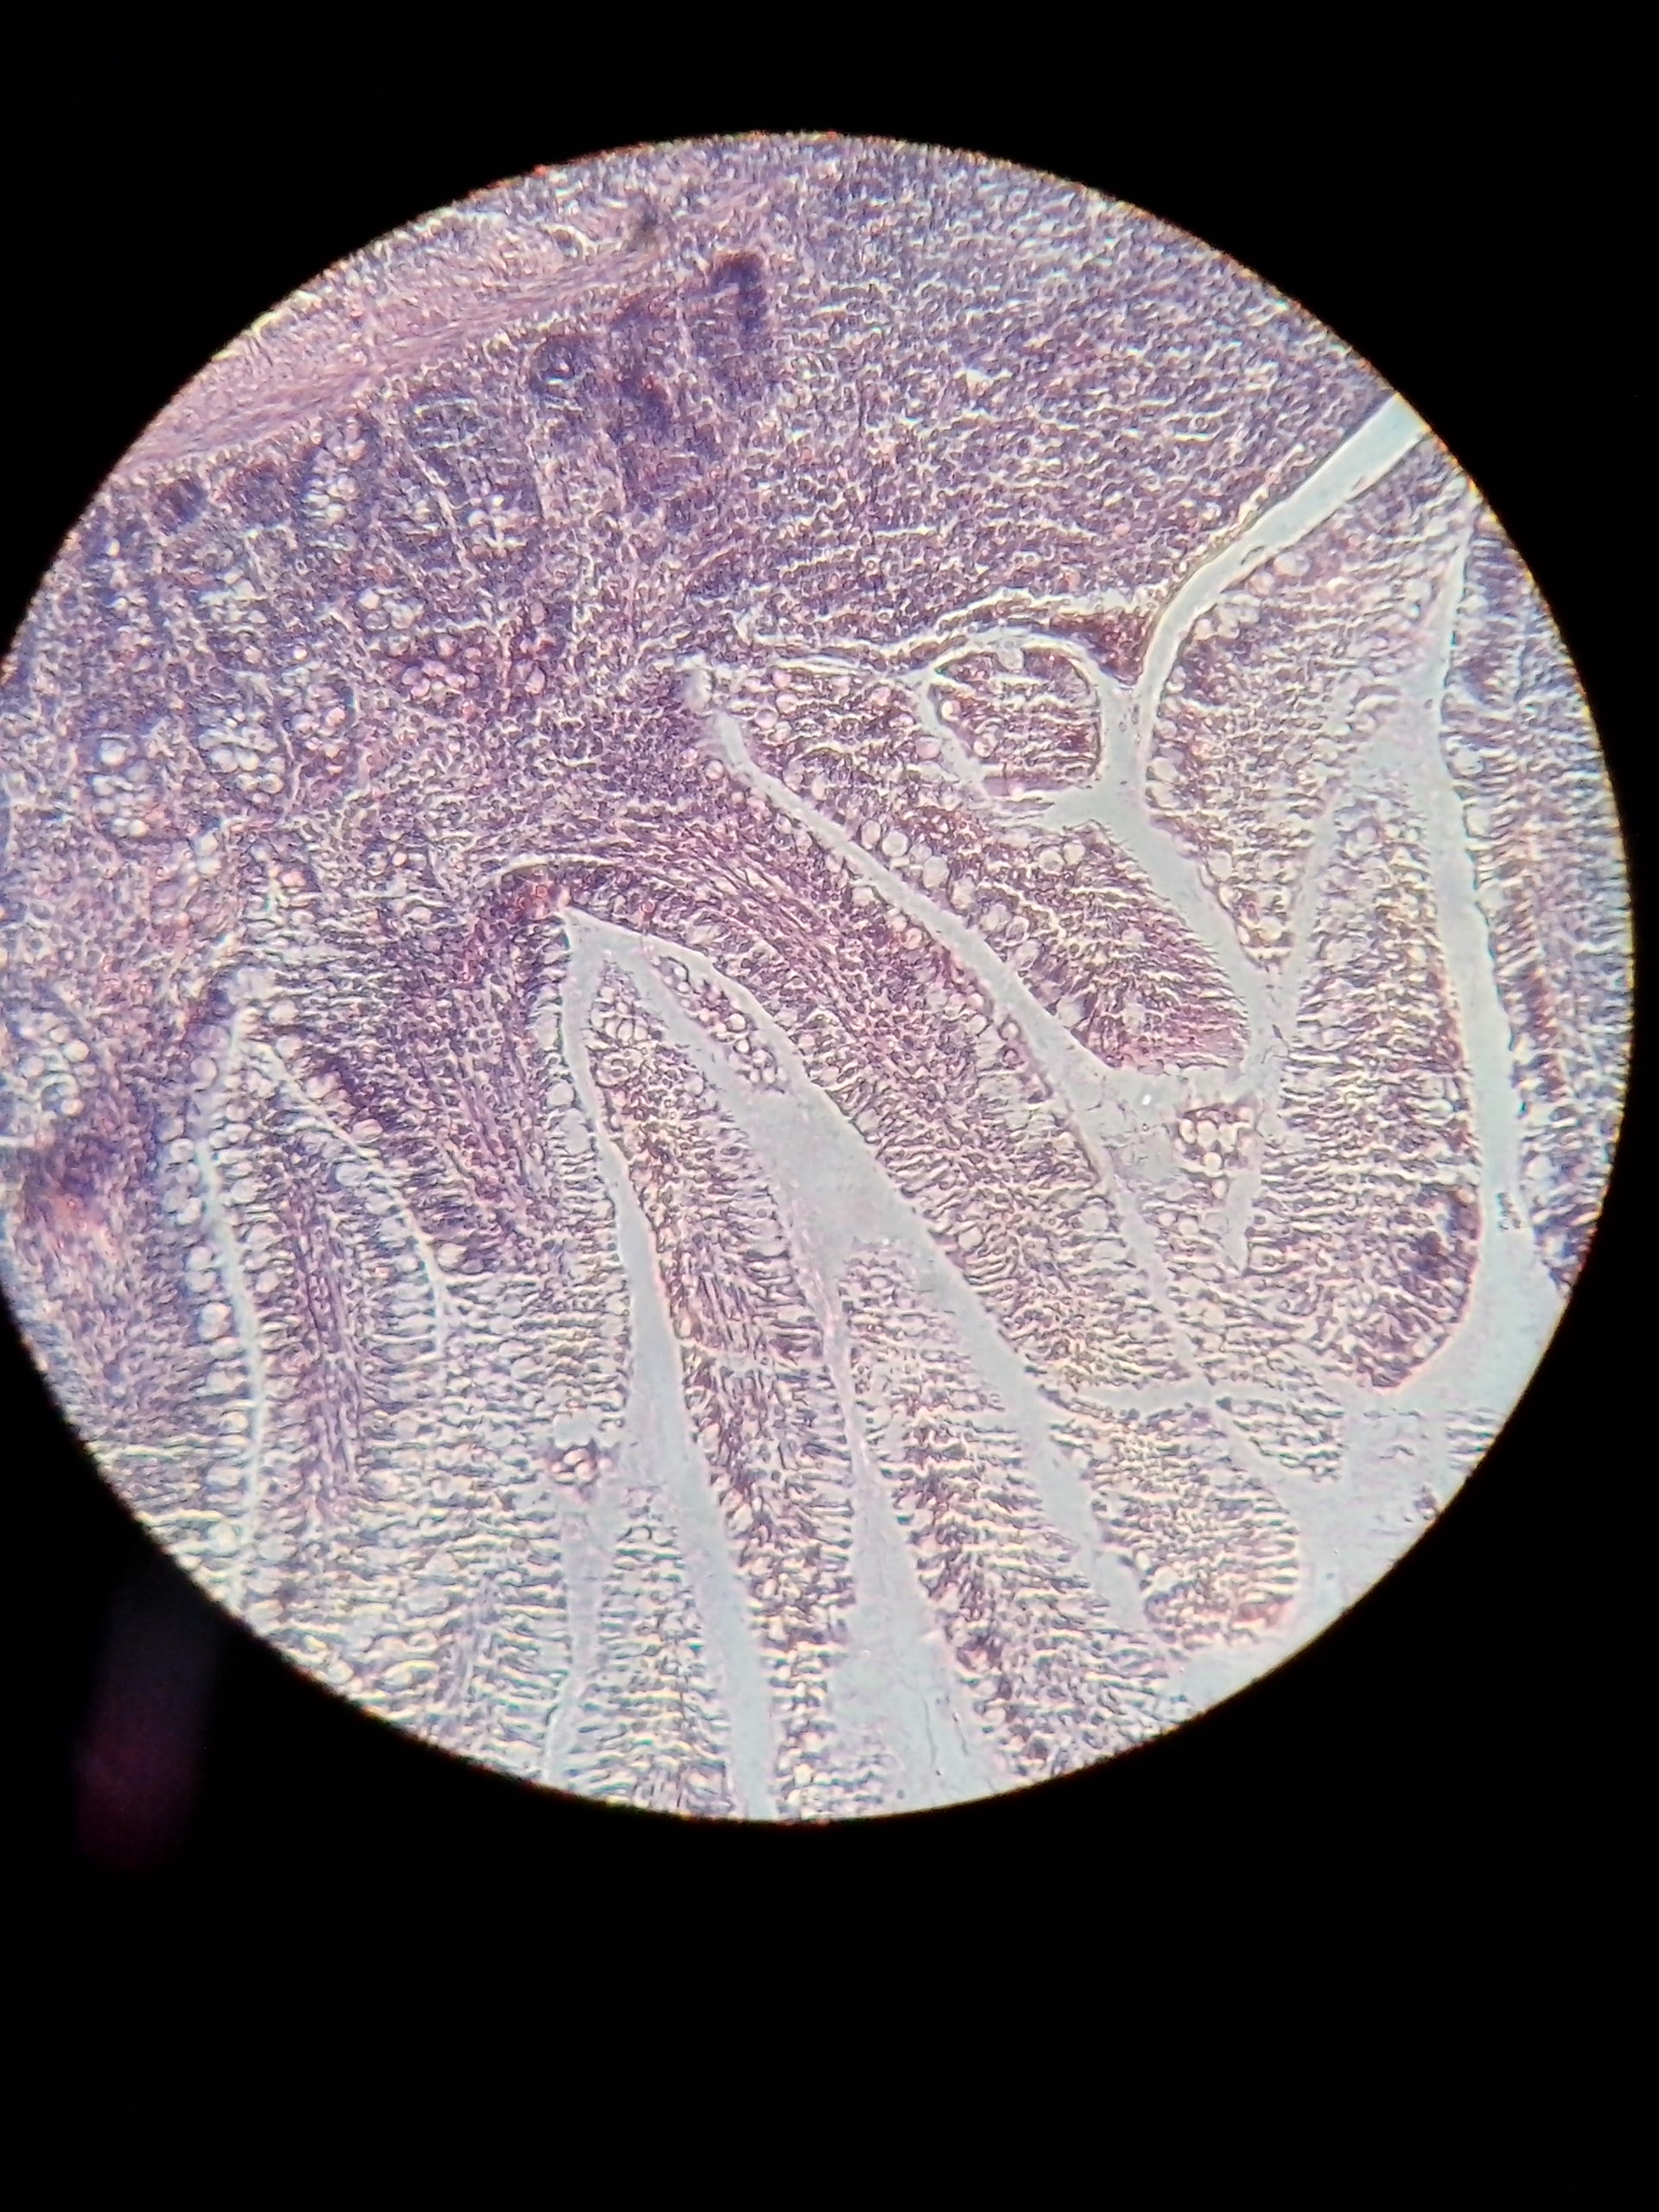
\includegraphics[width=1\textwidth]{../images/04_mammal_illeum.jpg}
		\caption{Objektiv 20x}
		\label{fig:04_mammal_ileum}
	\end{subfigure}
	\begin{subfigure}[b]{0.3\textwidth}
		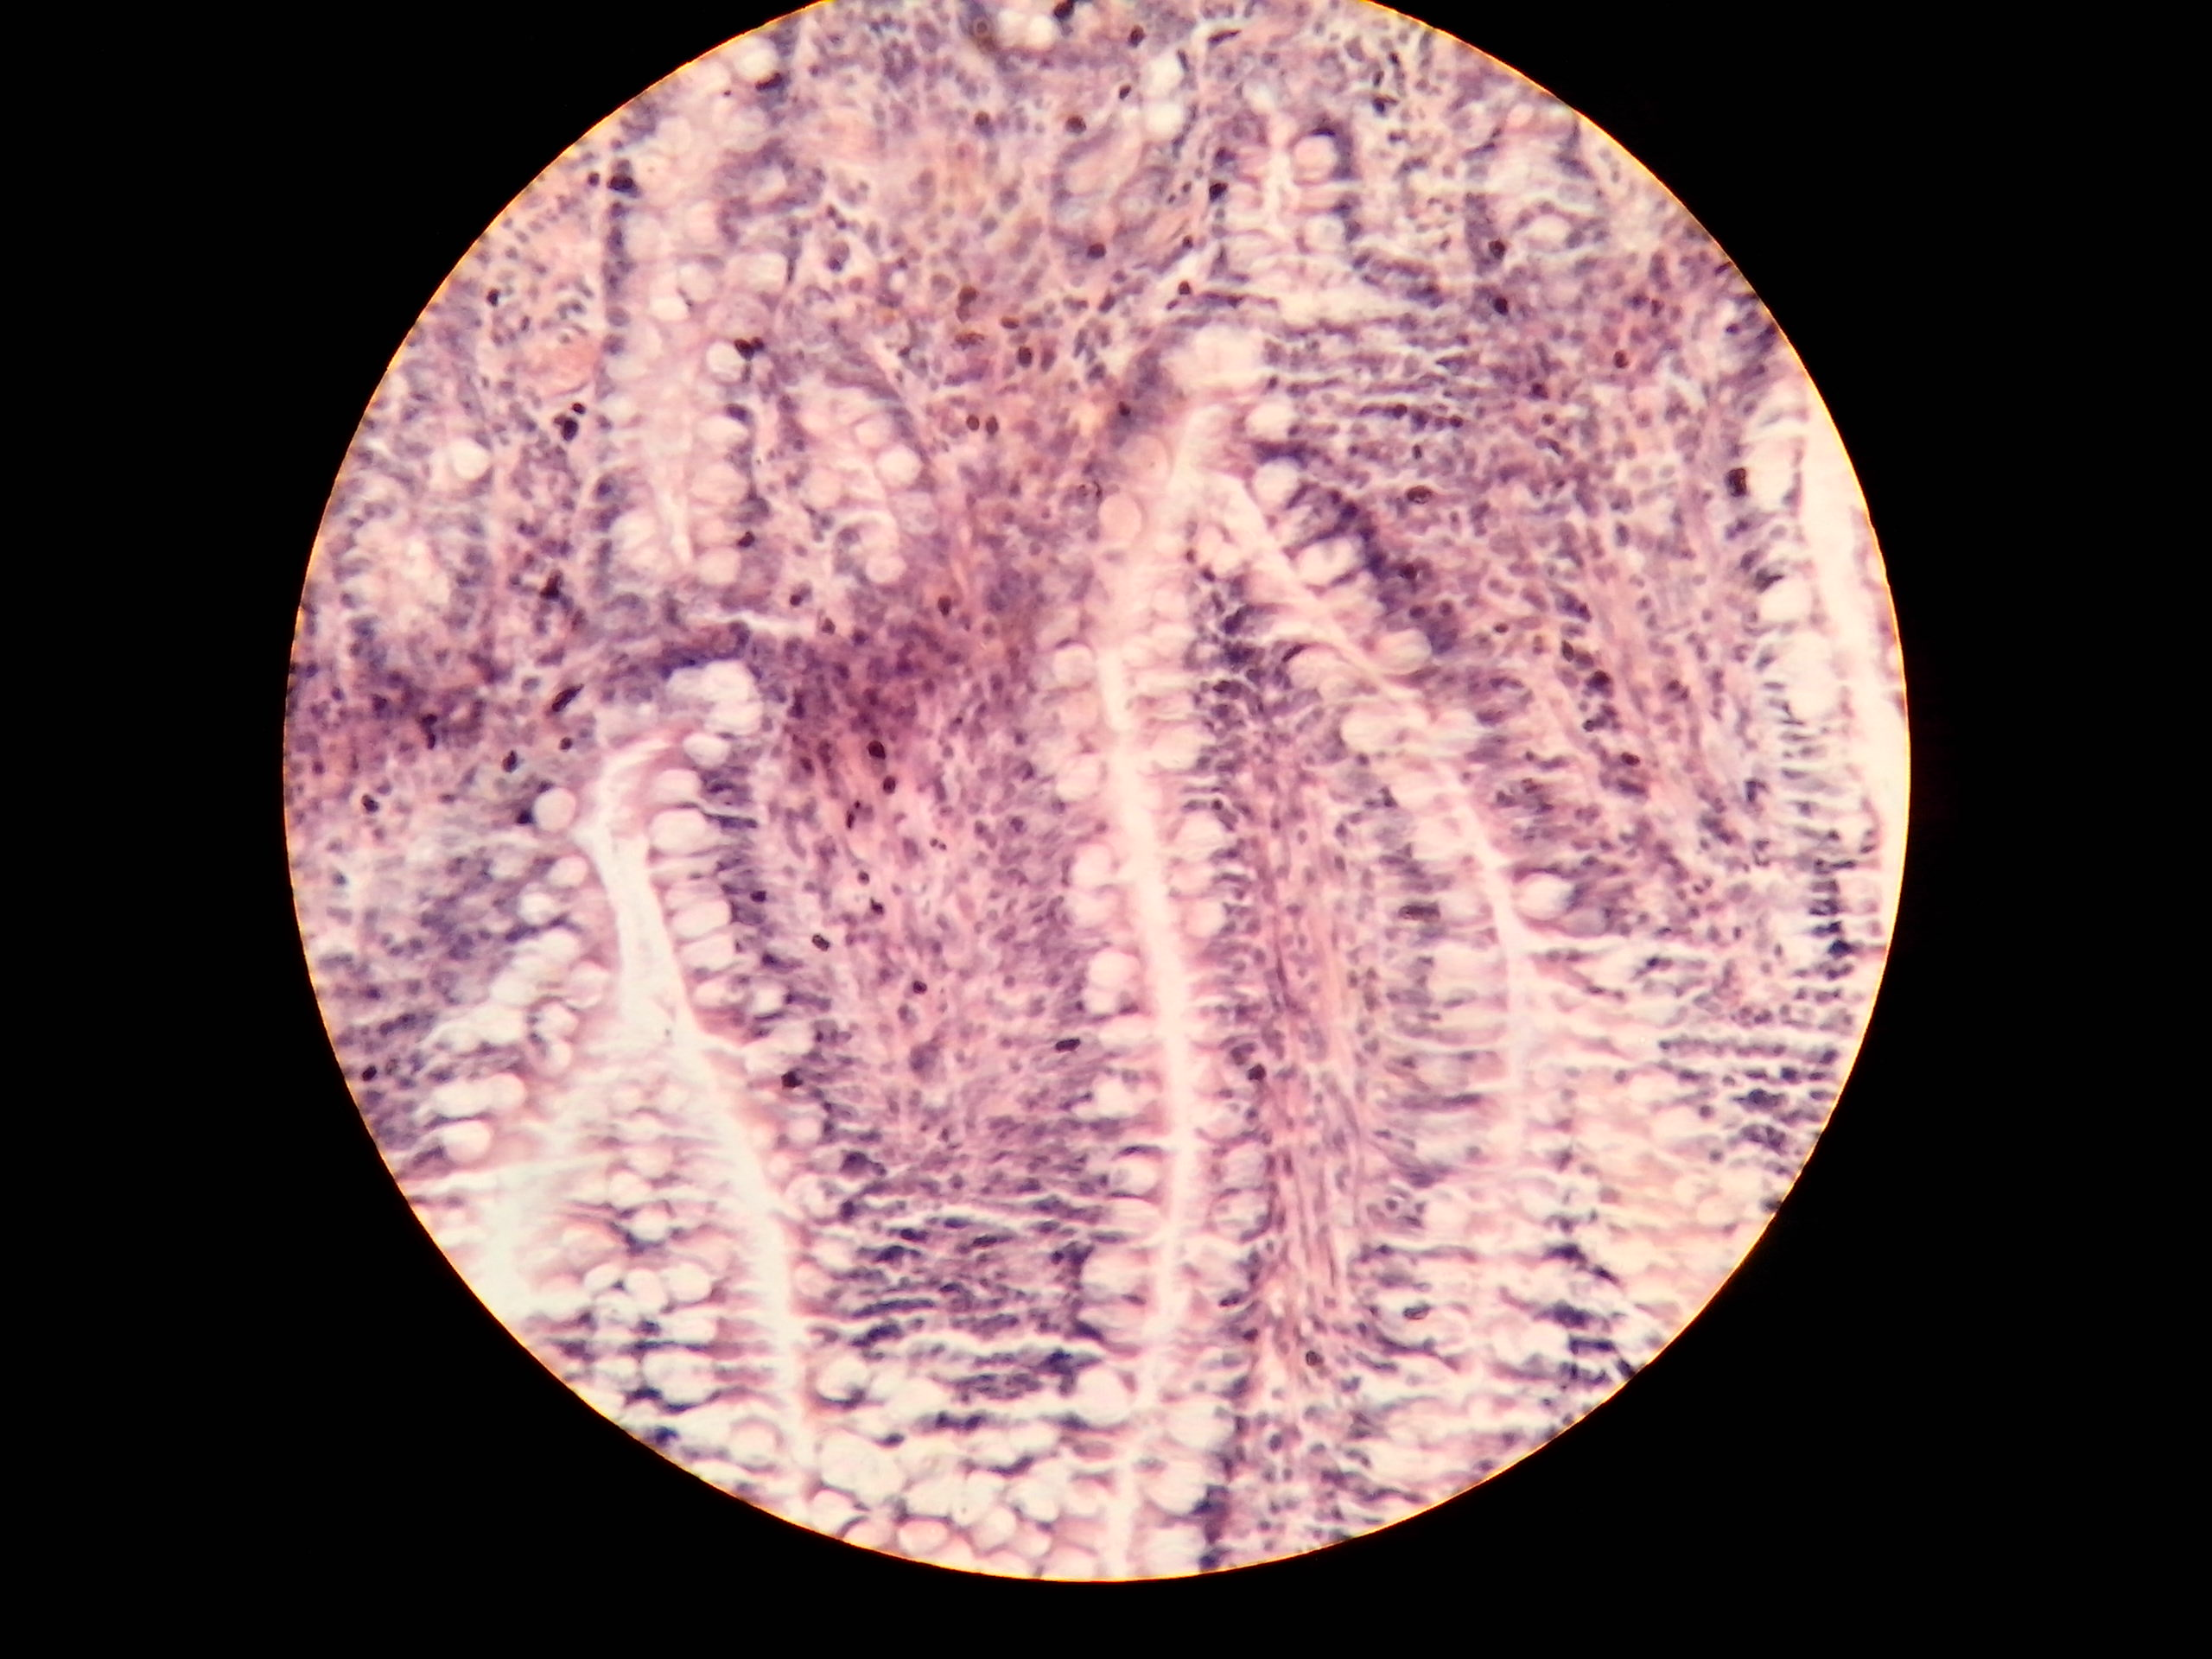
\includegraphics[angle=270, width=1\textwidth]{../images/05_mammal_illeum.jpg}
		\caption{Objektiv 40x}
		\label{fig:05_mammal_ileum}
	\end{subfigure}
	\begin{subfigure}[b]{0.3\textwidth}
		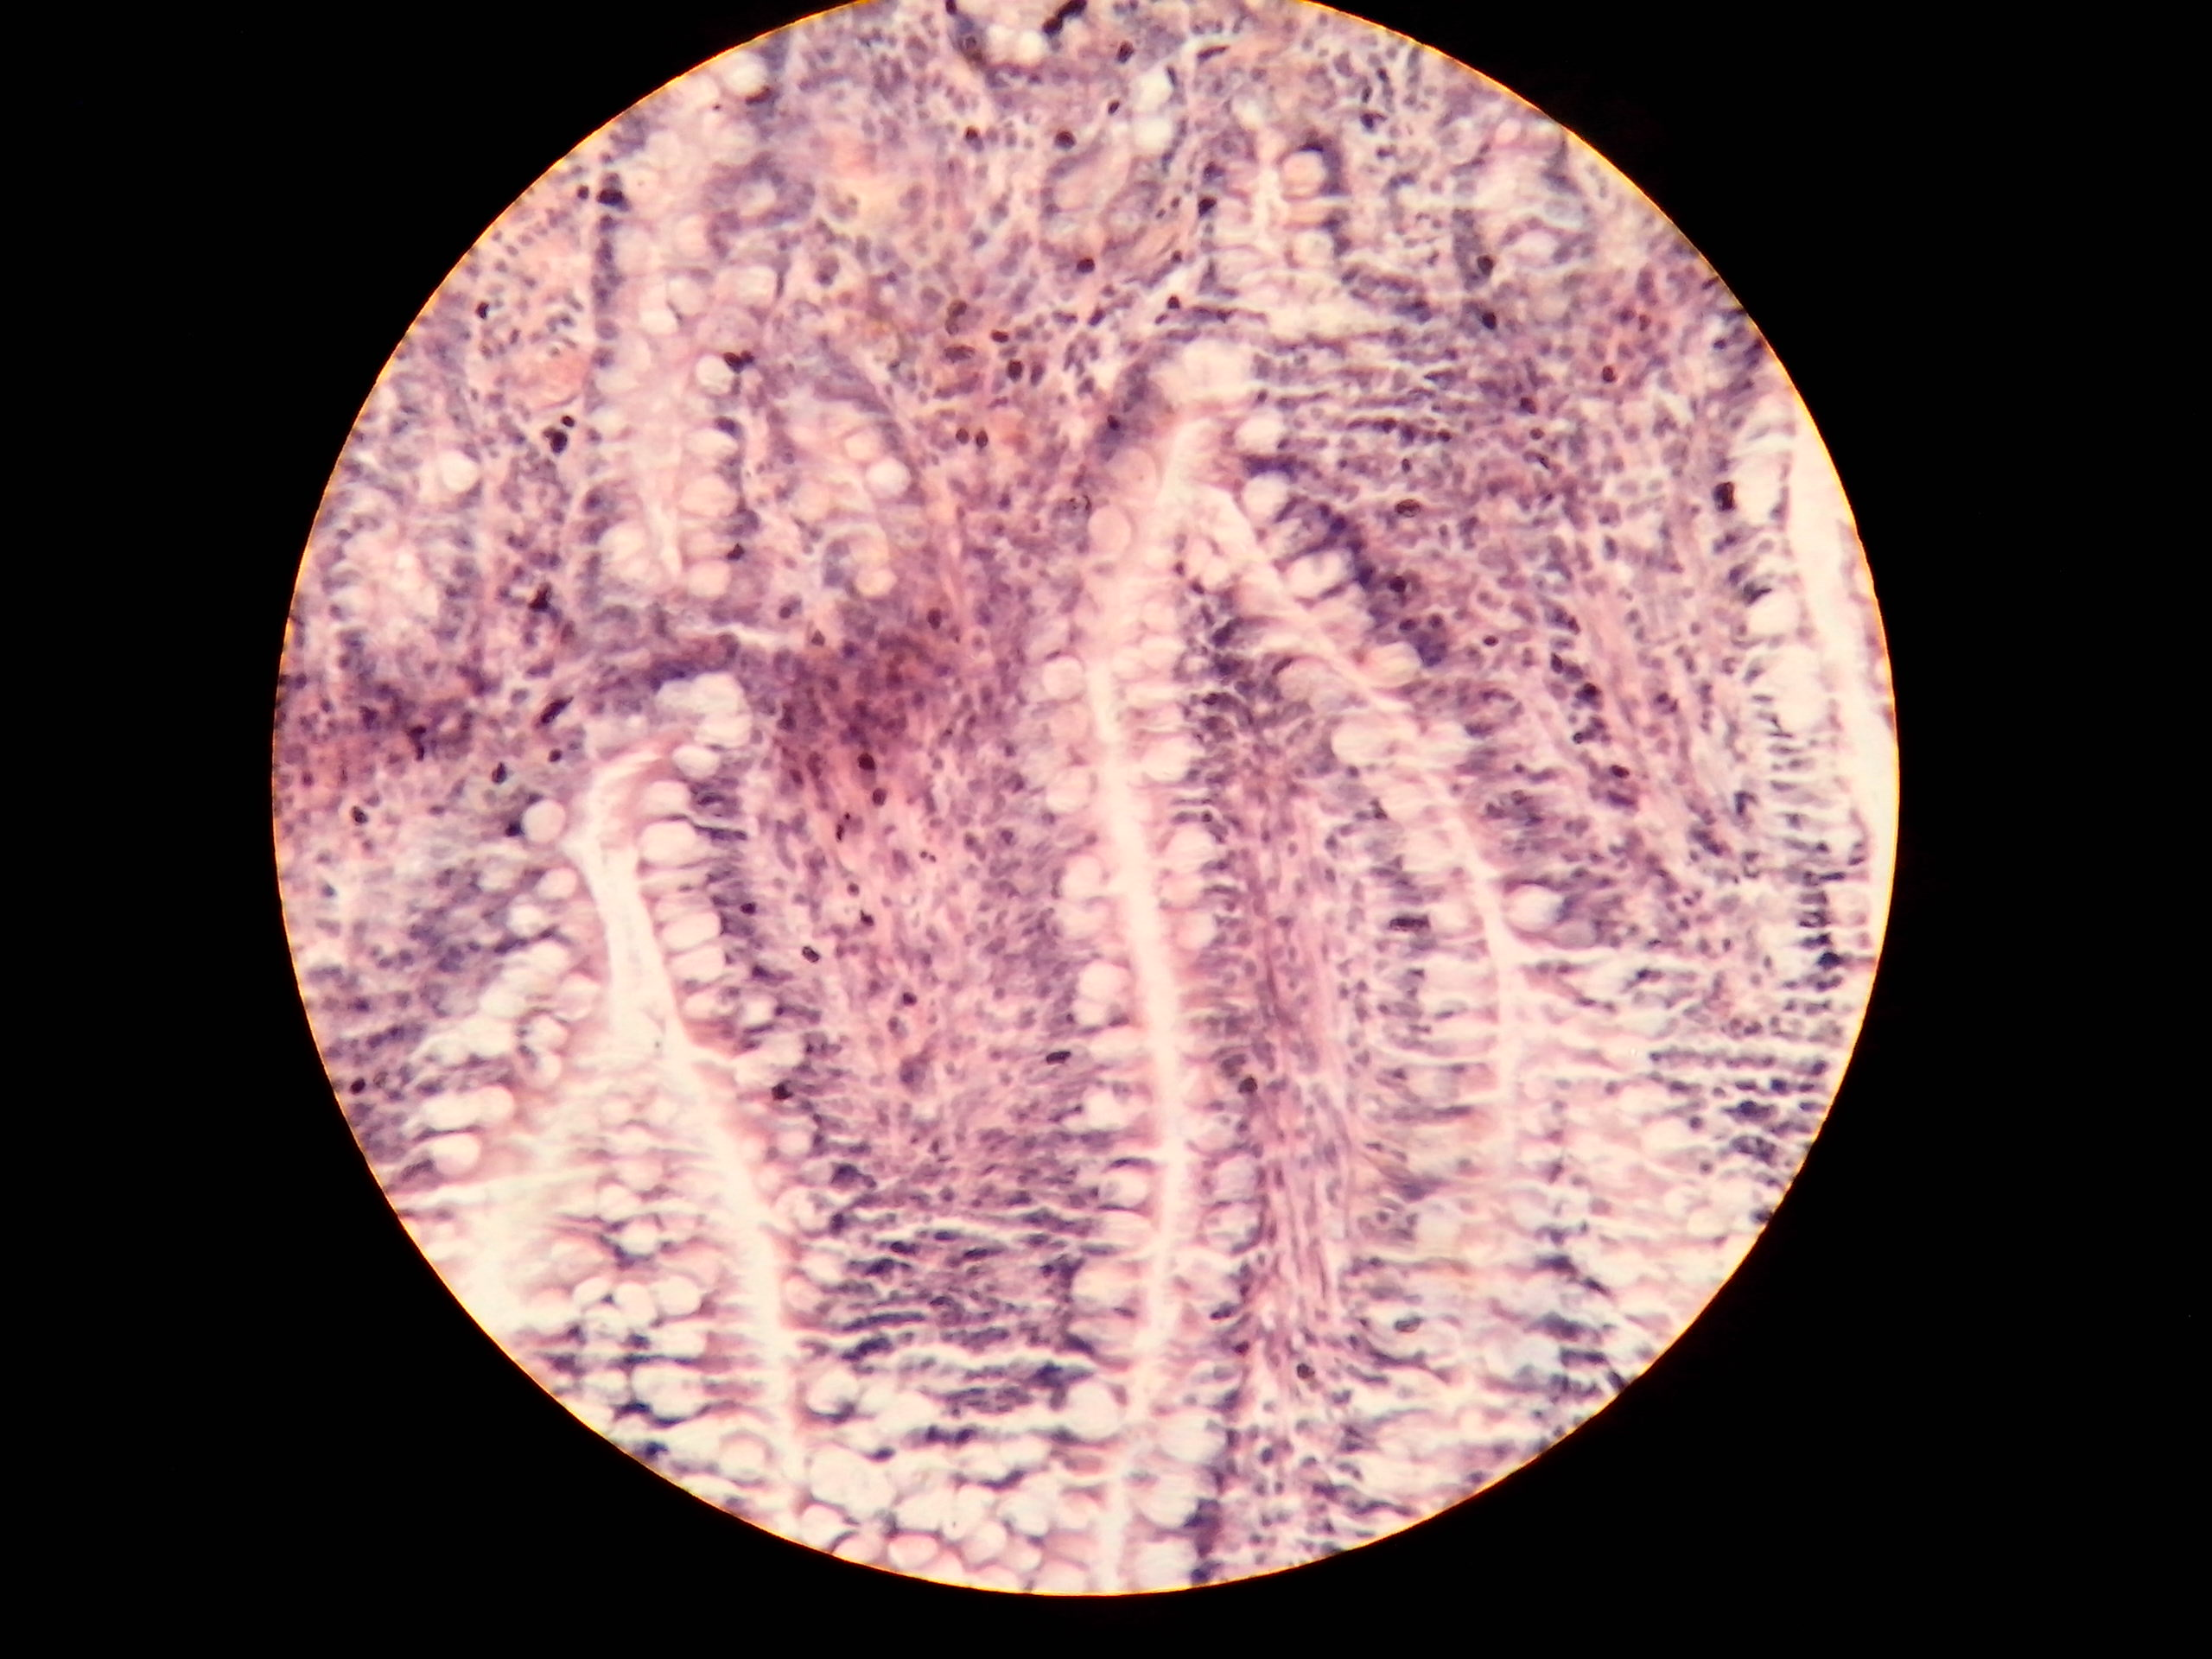
\includegraphics[angle=270, width=1\textwidth]{../images/06_mammal_illeum.jpg}
		\caption{Objektiv 40x}
		\label{fig:06_mammal_ileum}
	\end{subfigure}
	\caption{Aufzeichnungen der Lichtmikorskopischen Darstellungen der
		Dünndarmproben}
	\label{fig:mammal_ileum}
\end{figure}

\subsubsection{Kommentar}
Die Abbildungen \ref{fig:01_mammal_ileum} bis \ref{fig:06_mammal_ileum}
zeigen die auffällige Struktur der Schleimhaut des menschlichen Dünndarms.
Diese hat eine gefaltete Struktur, welche eine Zunahme der Gesamtoberfläche
zur Folge hat. Diese Faltungen oder auch Einsenkungen bilden die sogenannten
Lieberkühn-Drüsen \cite{wiki-leberkuehn-krypten}. Mit einer grösseren Fläche
der Schleimhaut kann die Reaktion mit dem durchgehenden Nahrungsbrei
effizienter erfolgen. Inbesondere die Abbildungen \ref{fig:05_mammal_ileum}
und \ref{fig:06_mammal_ileum} zeigen diese deutlich auf.

\newpage
\subsection{Menschliche Leber}

\subsubsection{Proben}
\begin{table}[h!]
	\centering
	\begin{tabular}{l l}
		Bezeichnung	& Human liver \\
		Probe 		& 31-5388
	\end{tabular}
\end{table}

\subsubsection{Aufzeichnungen}
\begin{figure}[h!]
	\centering
	\begin{subfigure}[b]{0.3\textwidth}
		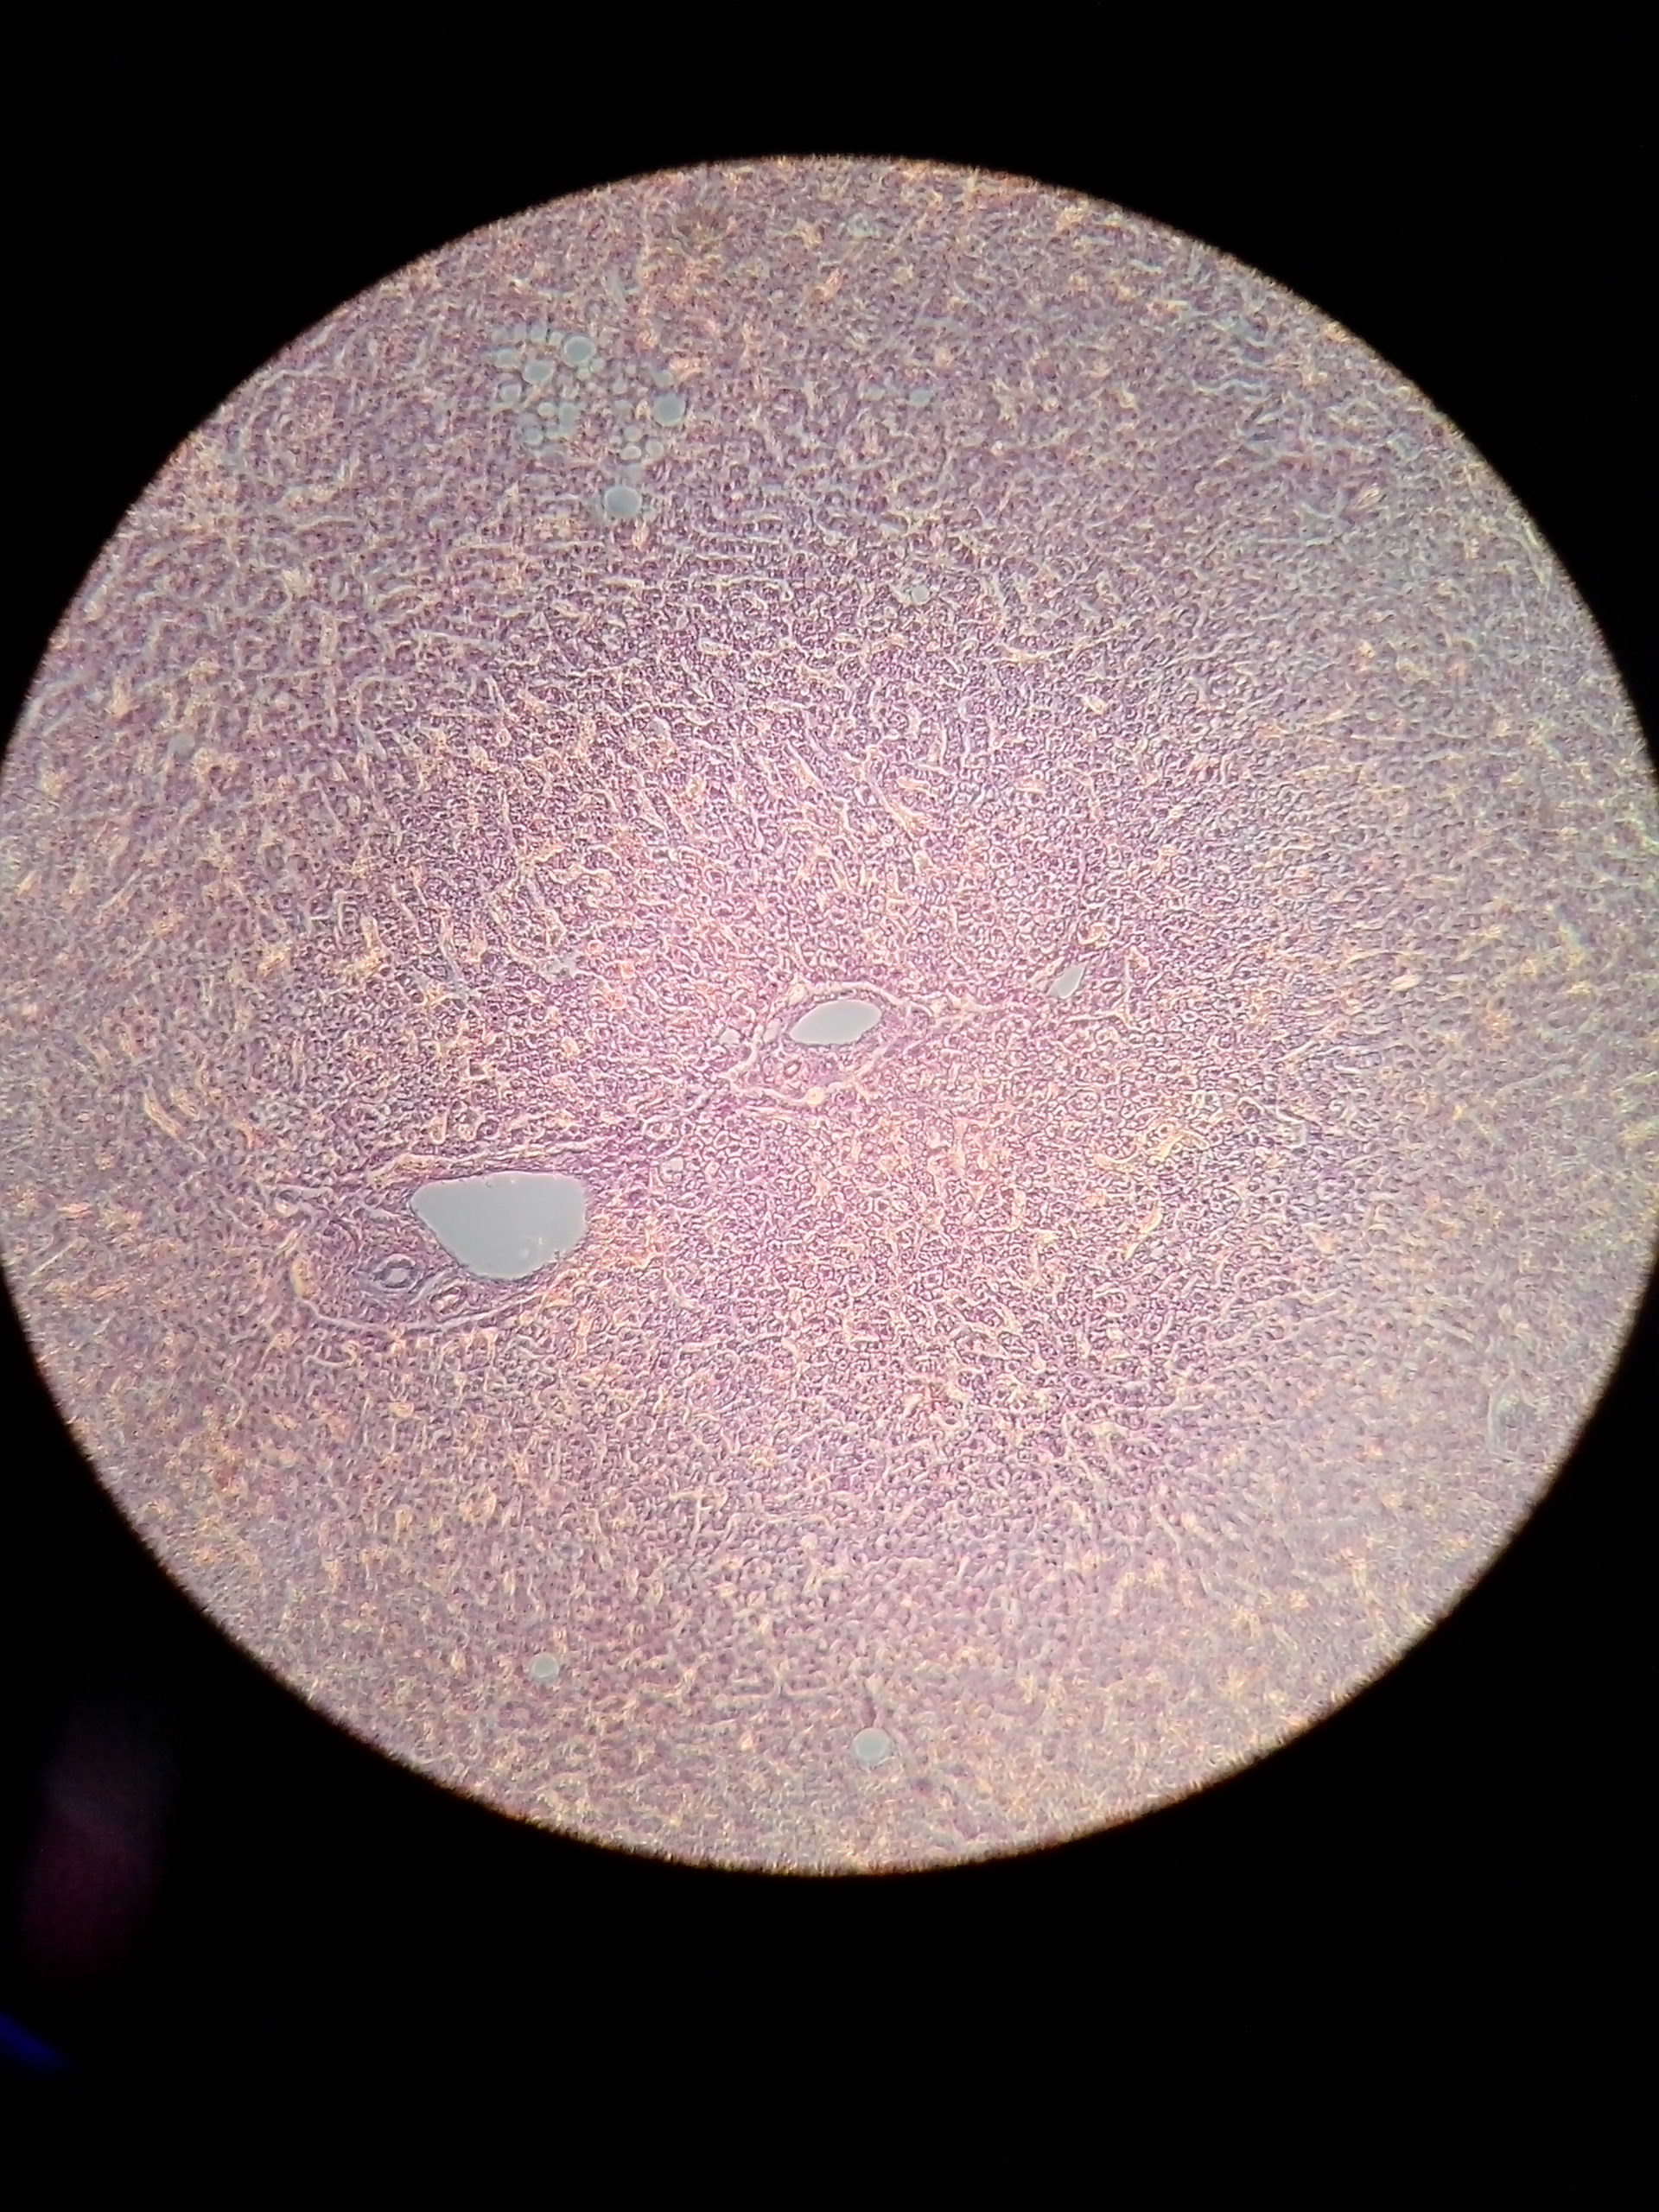
\includegraphics[width=1\textwidth]{../images/01_human_liver.jpg}
		\caption{Objektiv 10x}
		\label{fig:01_human_liver}
	\end{subfigure}
	\begin{subfigure}[b]{0.3\textwidth}
		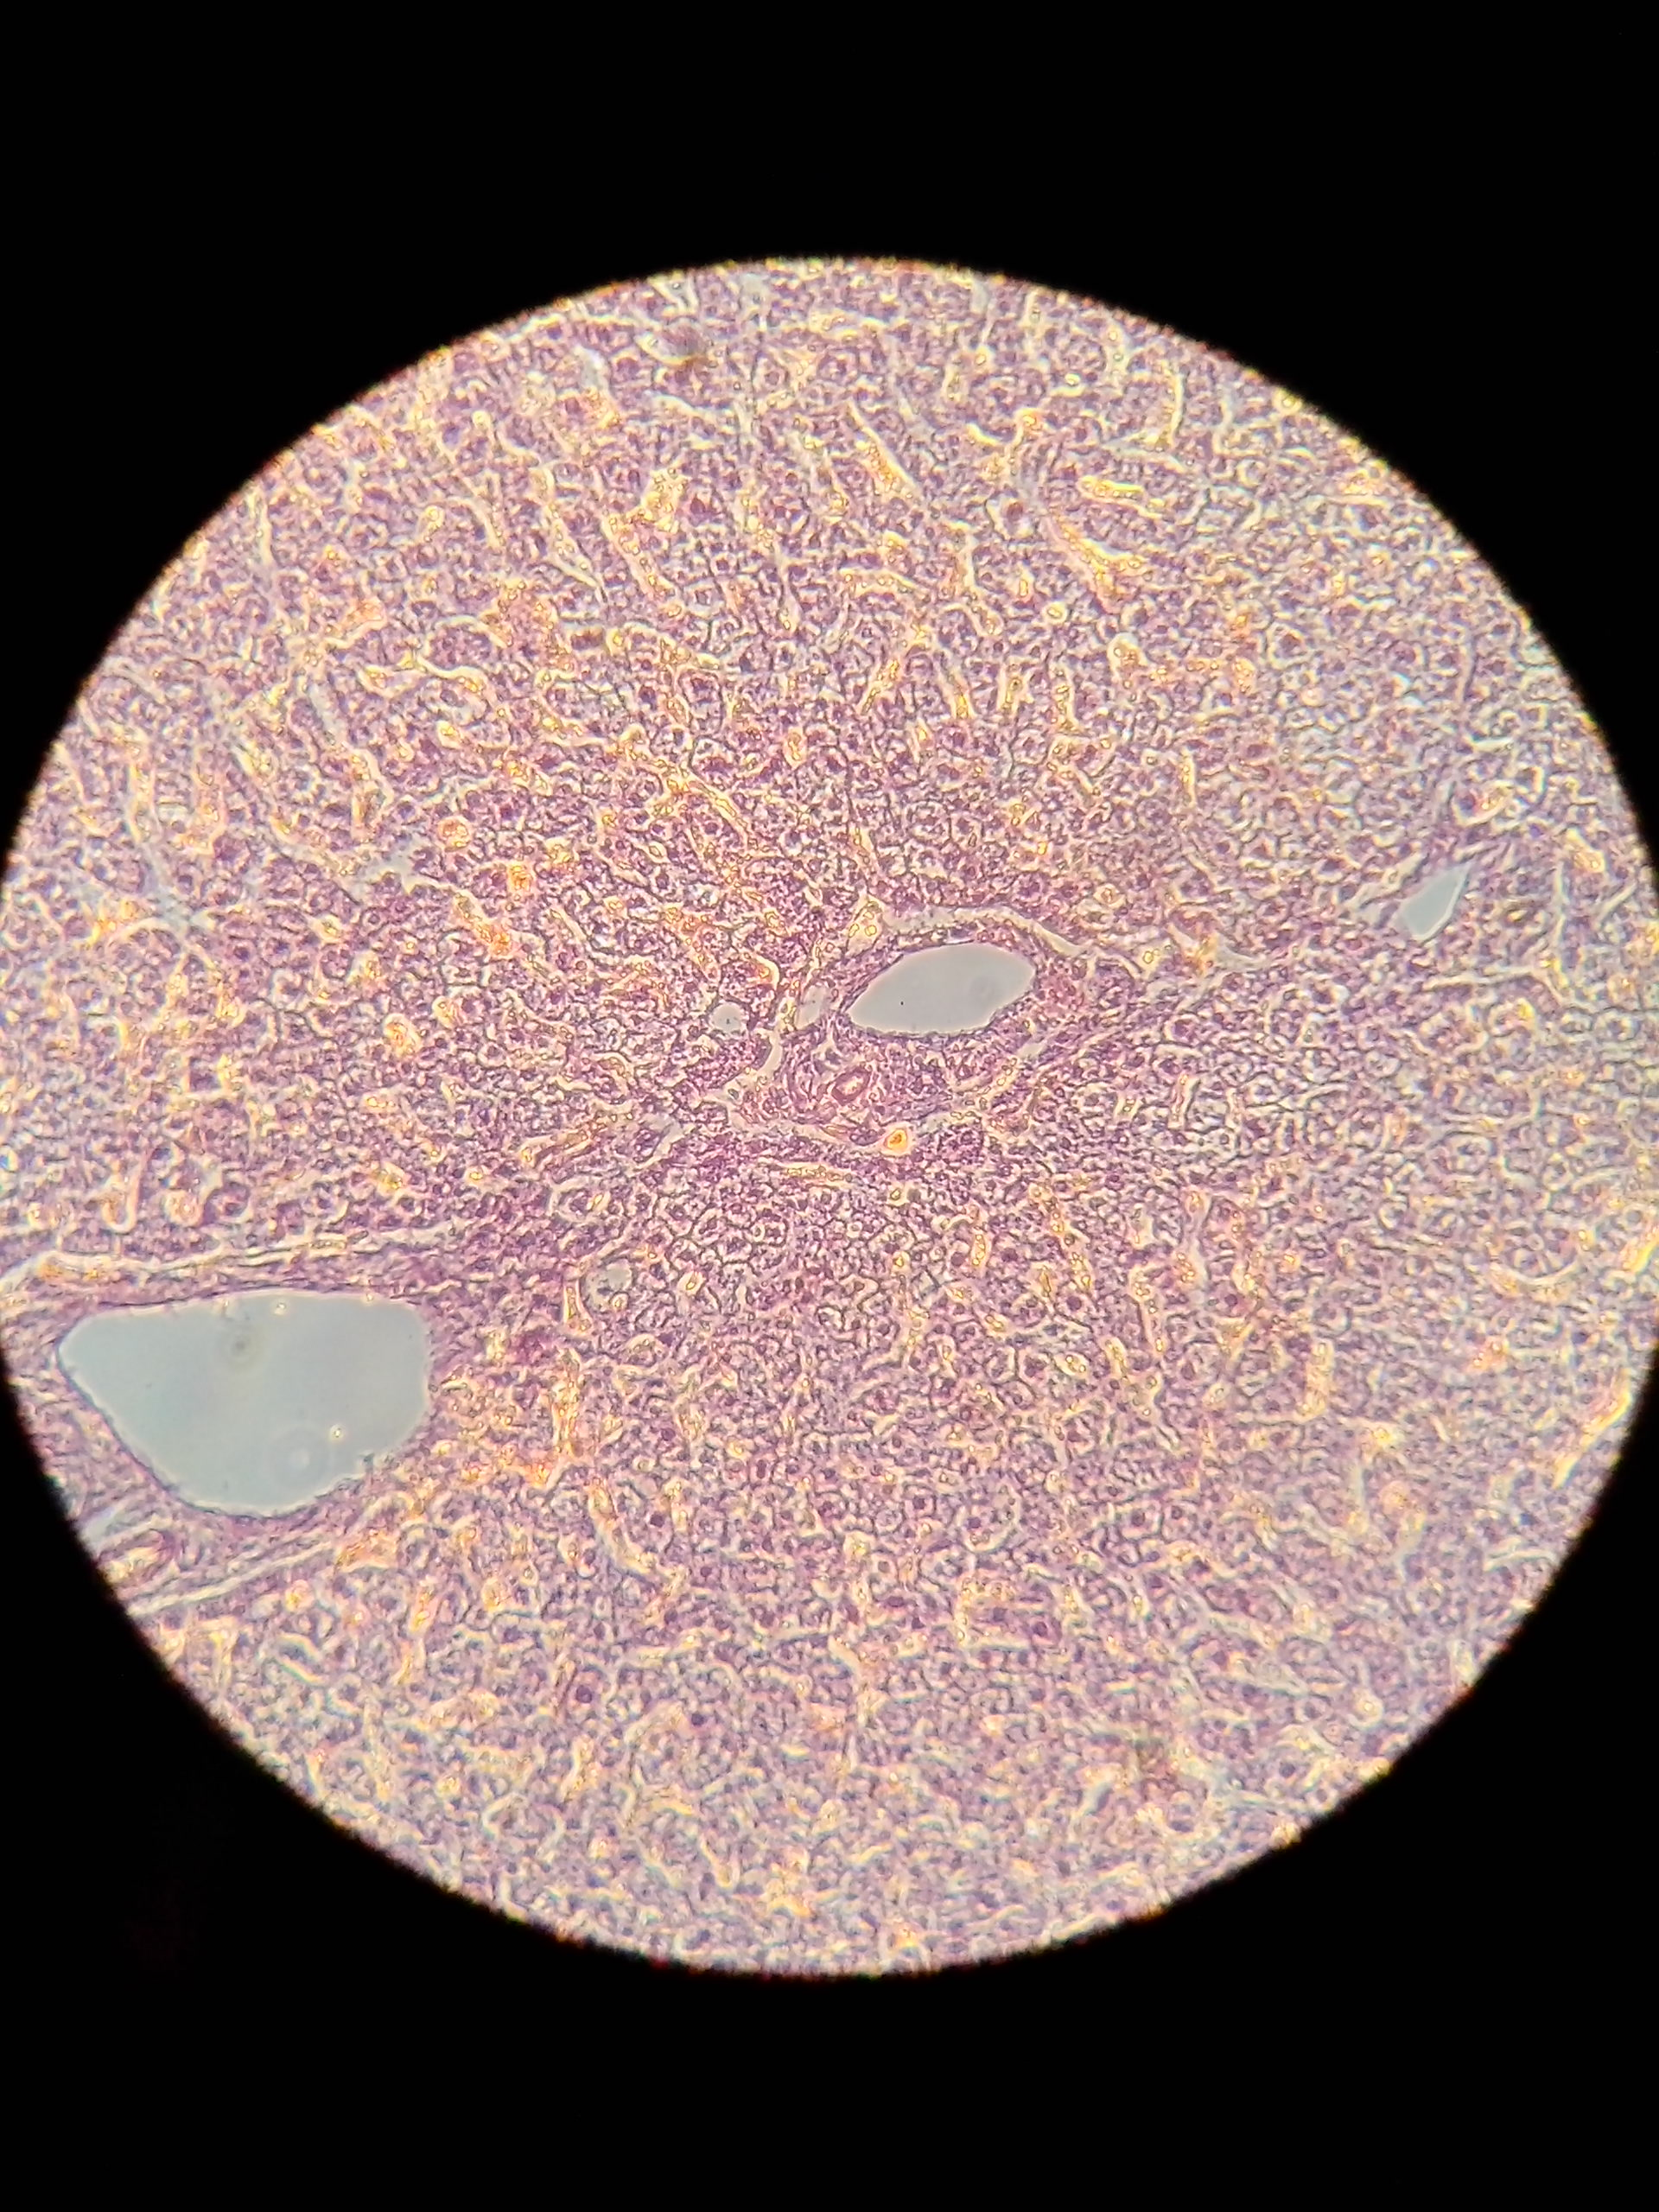
\includegraphics[width=1\textwidth]{../images/04_human_liver.jpg}
		\caption{Objektiv 20x}
		\label{fig:04_human_liver}
	\end{subfigure}
	\begin{subfigure}[b]{0.3\textwidth}
		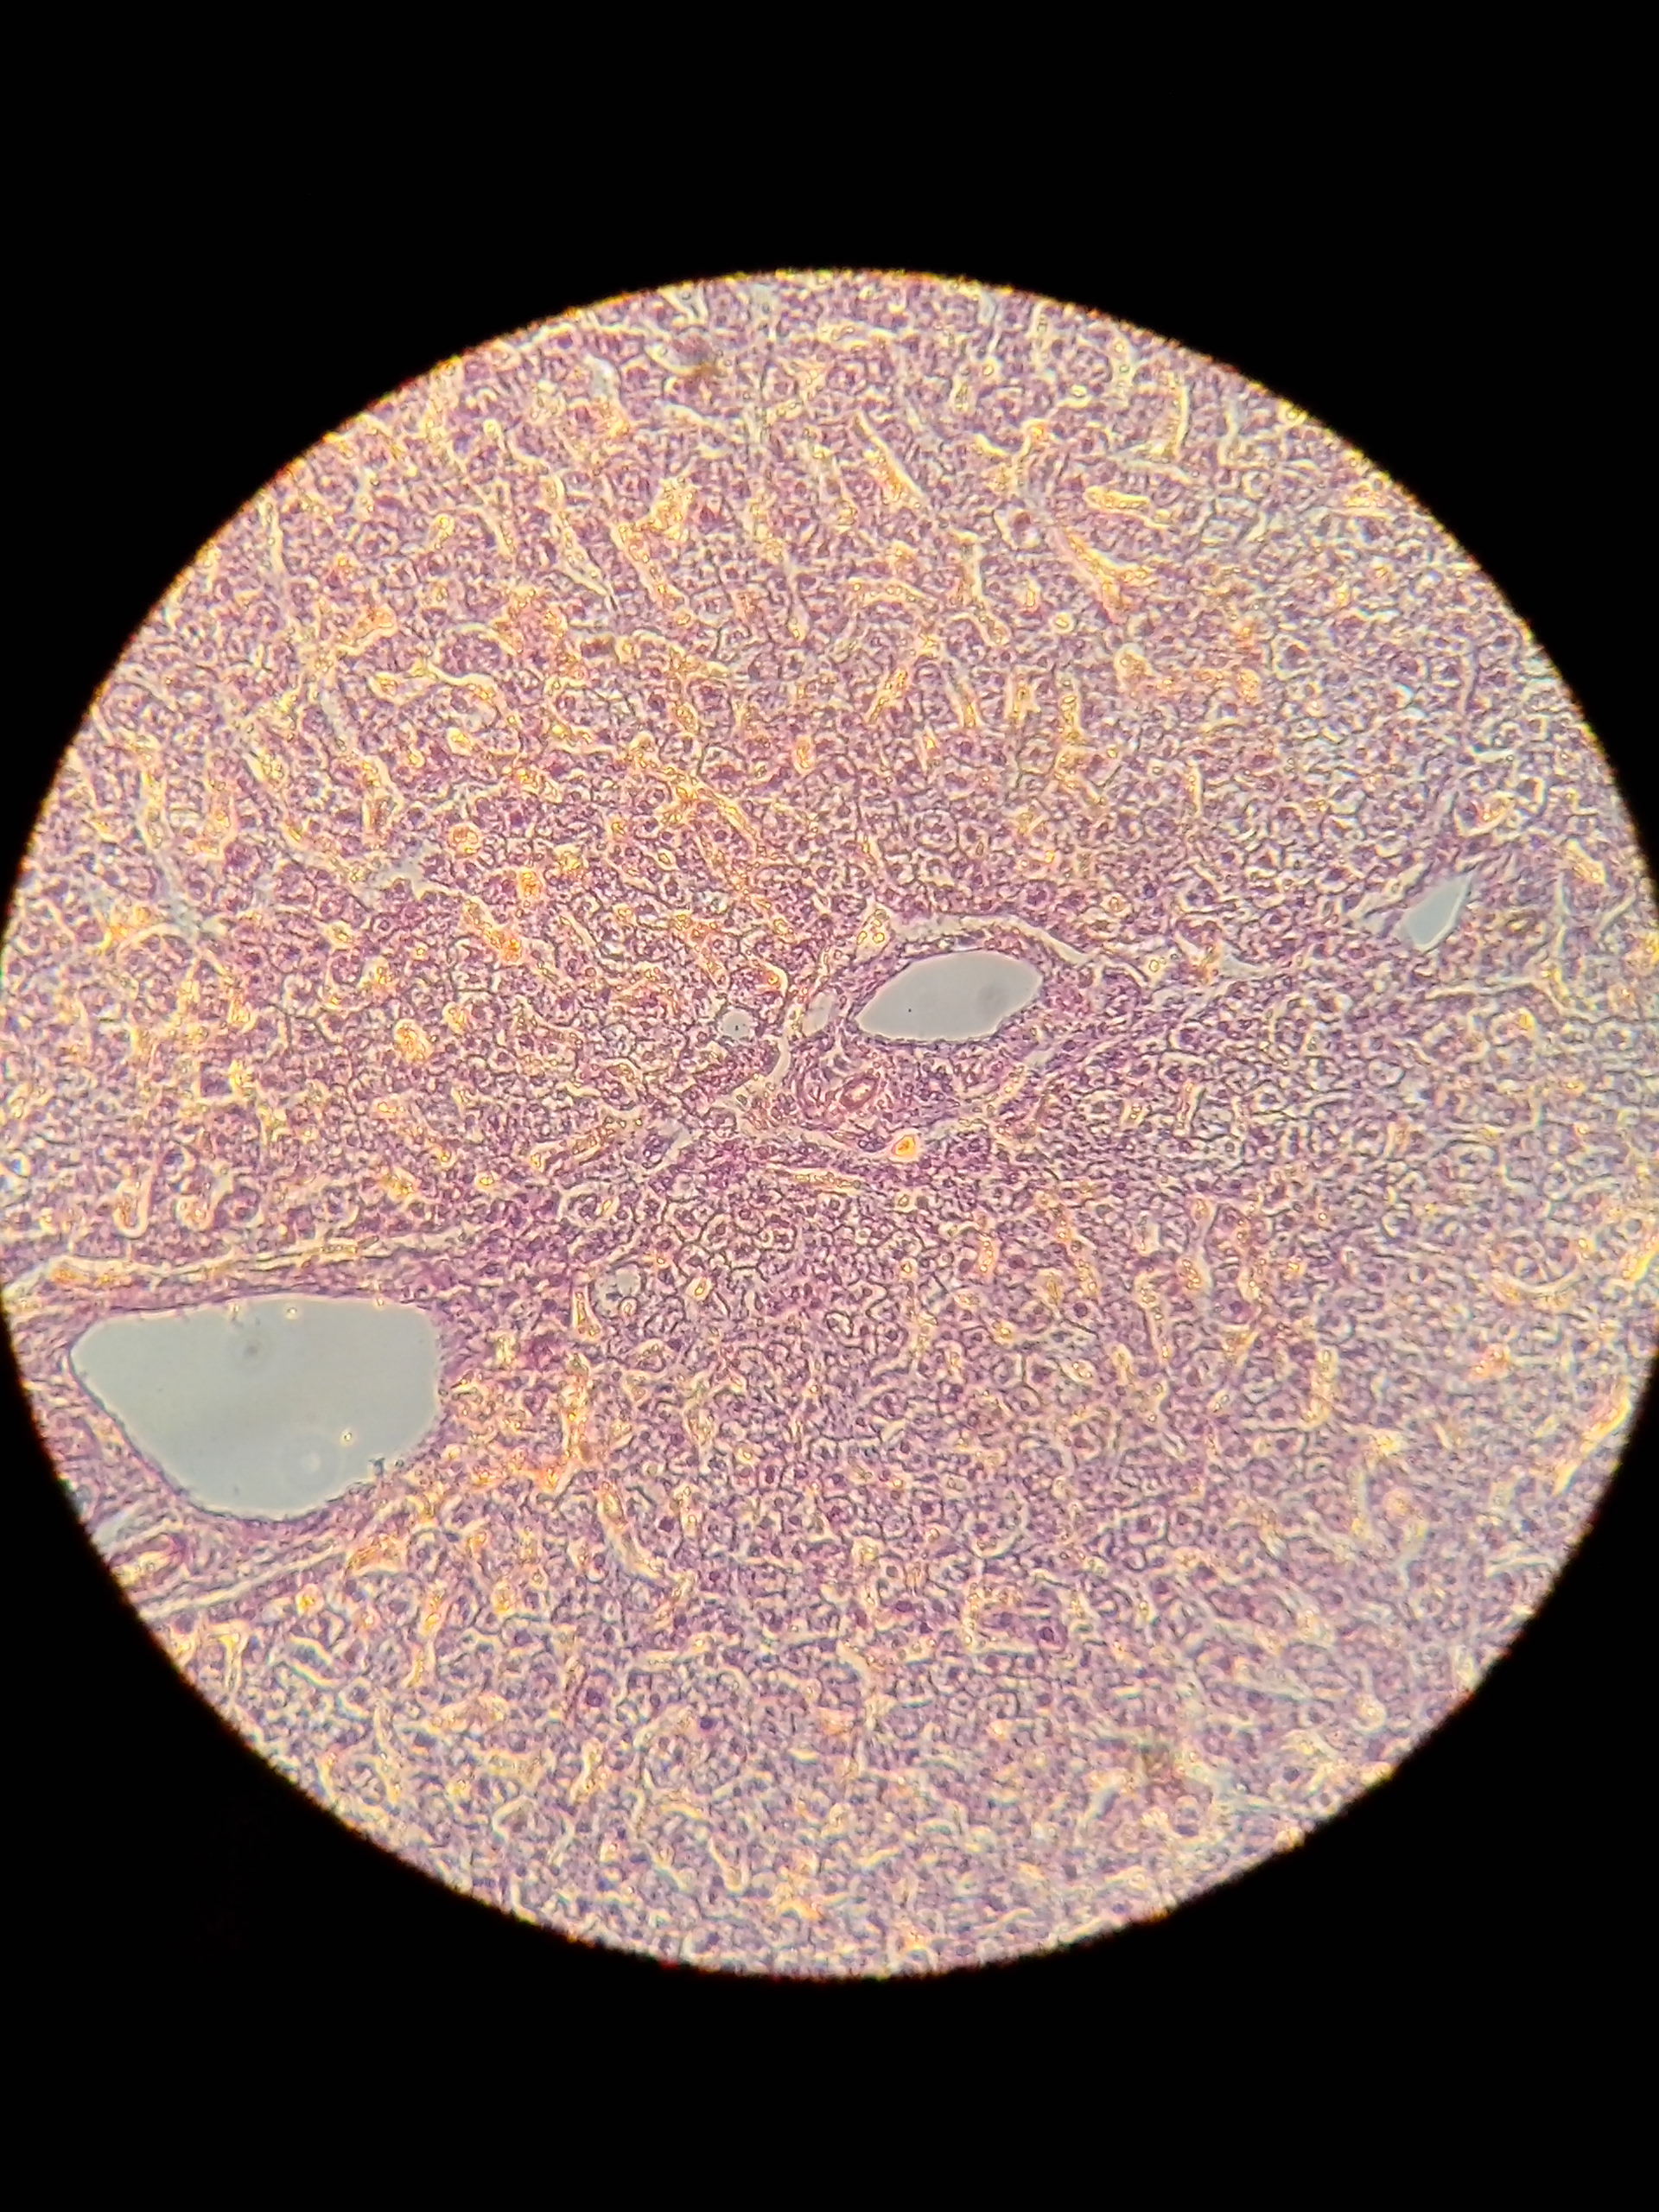
\includegraphics[width=1\textwidth]{../images/05_human_liver.jpg}
		\caption{Objektiv 20x}
		\label{fig:05_human_liver}
	\end{subfigure}

	\begin{subfigure}[b]{0.3\textwidth}
		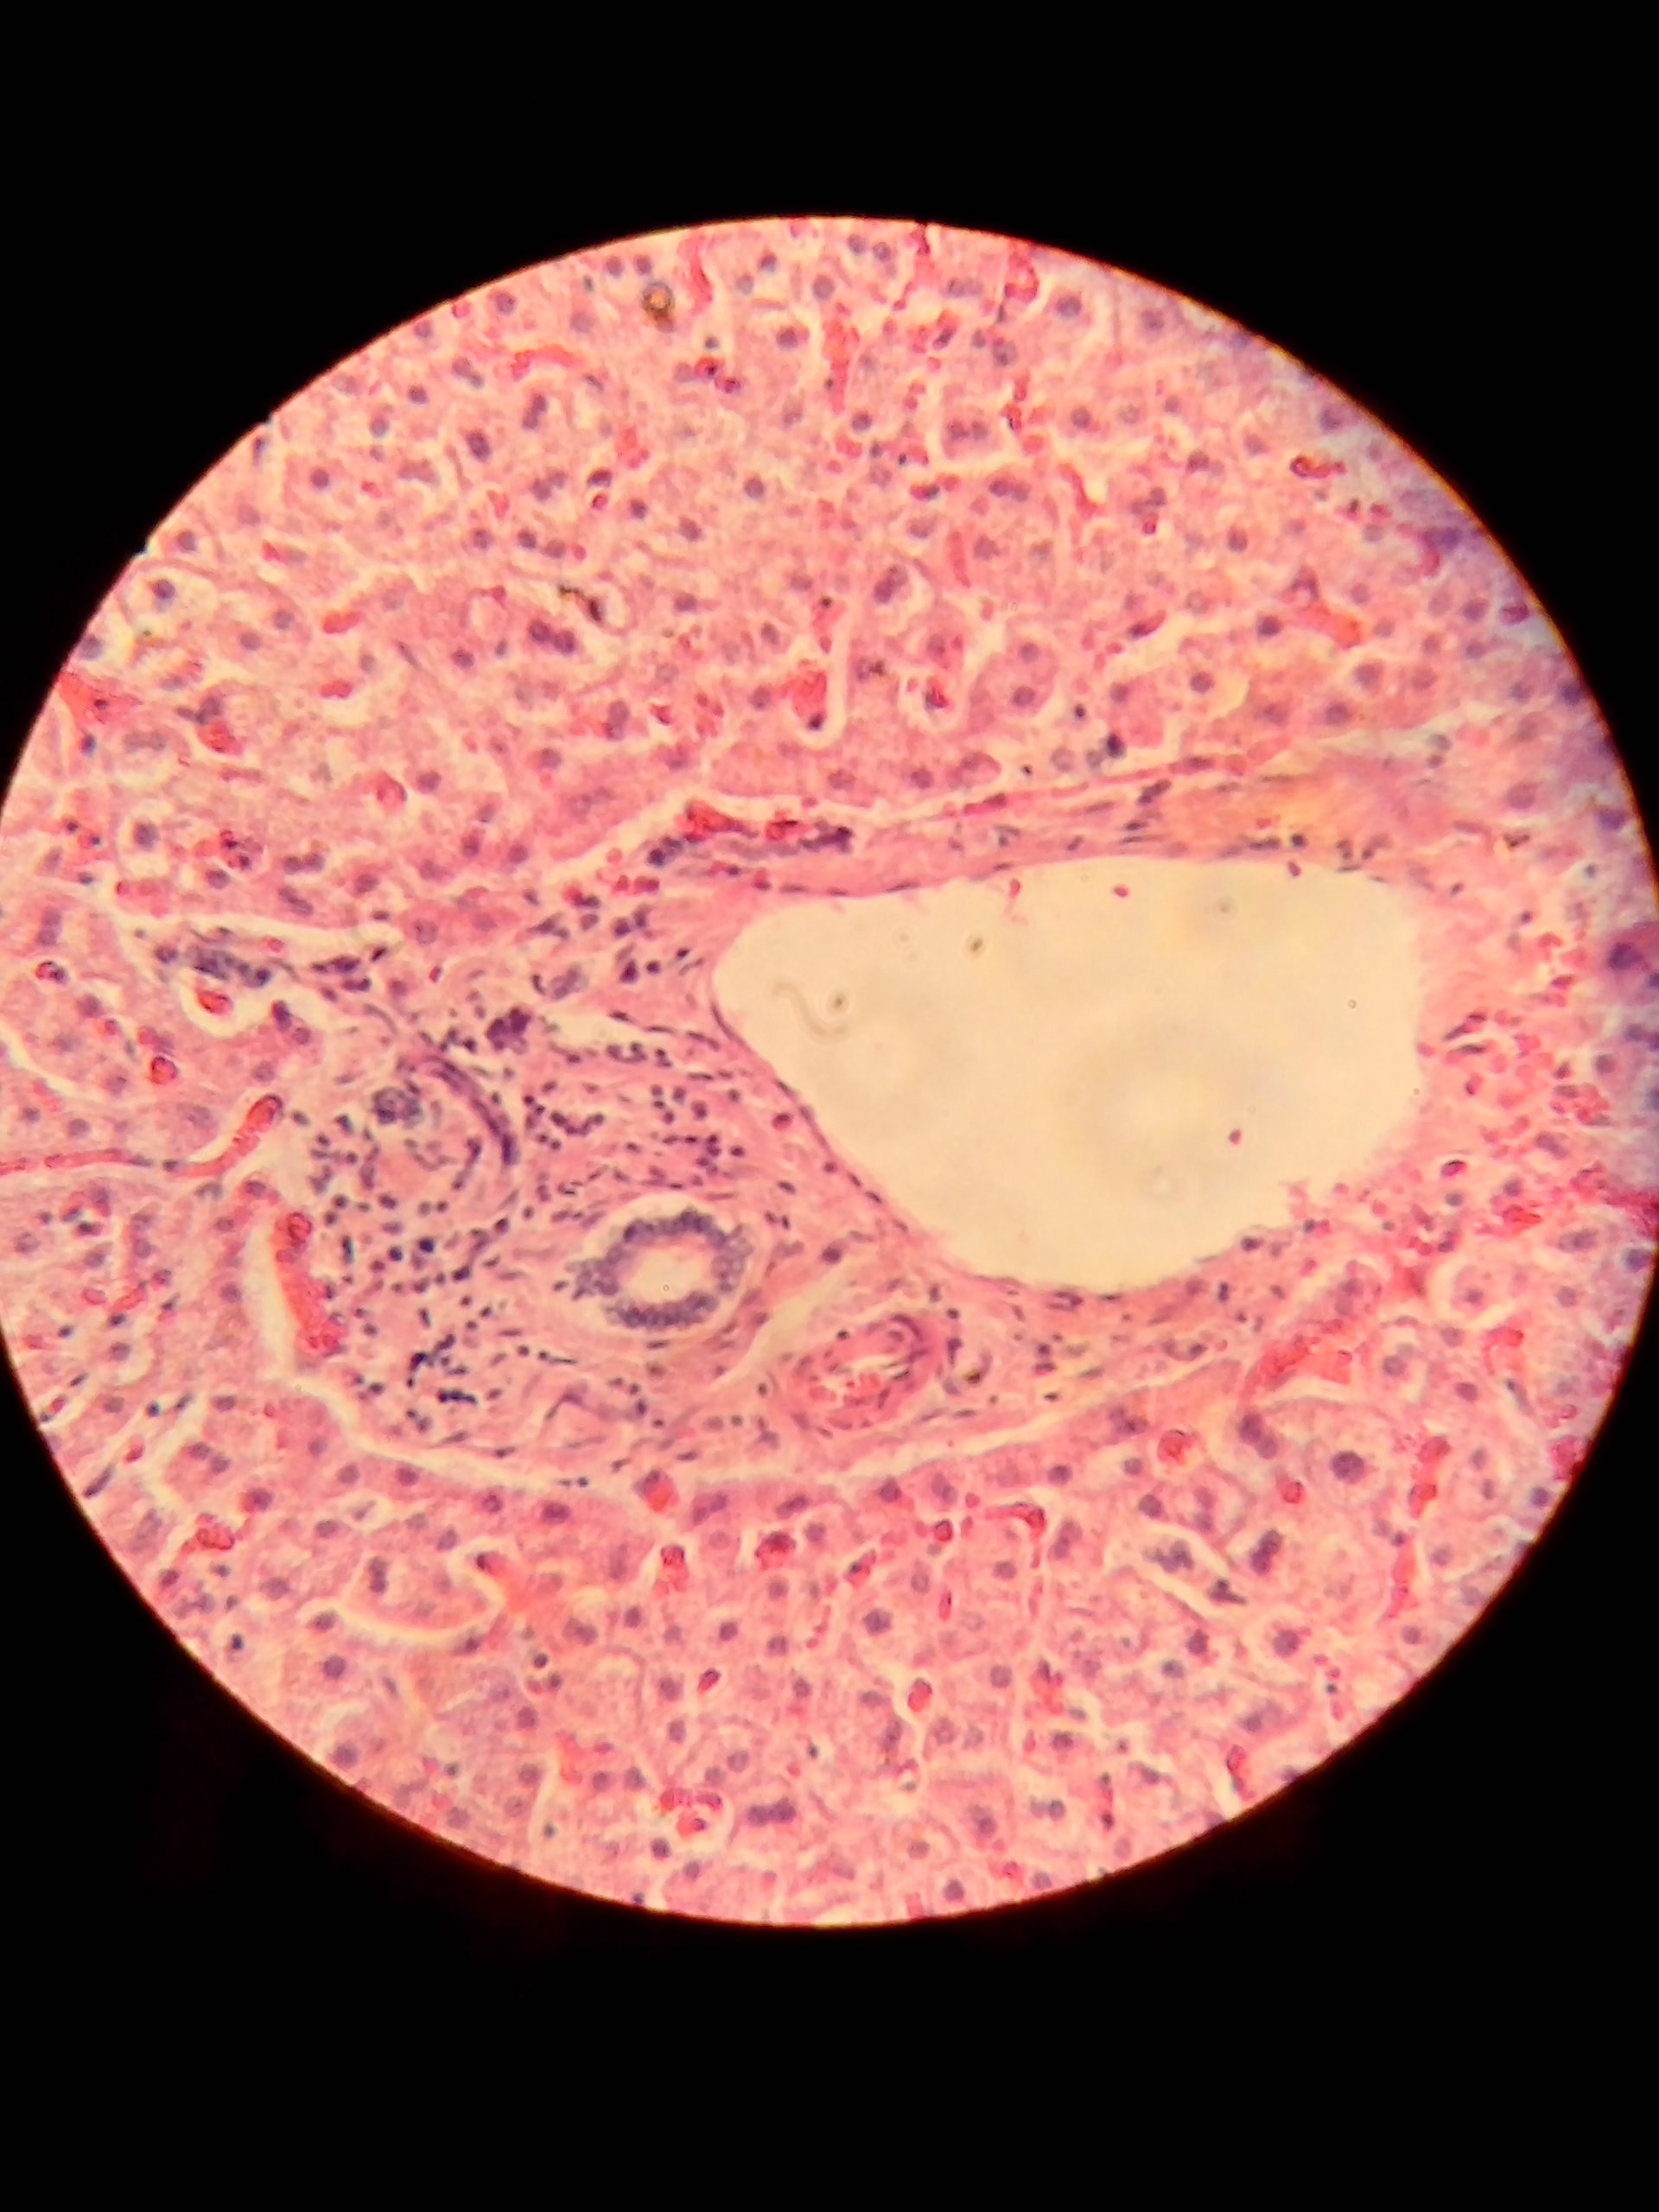
\includegraphics[width=1\textwidth]{../images/07_human_liver.jpg}
		\caption{Venengefäss -- Objektiv 40x}
		\label{fig:07_human_liver}
	\end{subfigure}
	\begin{subfigure}[b]{0.3\textwidth}
		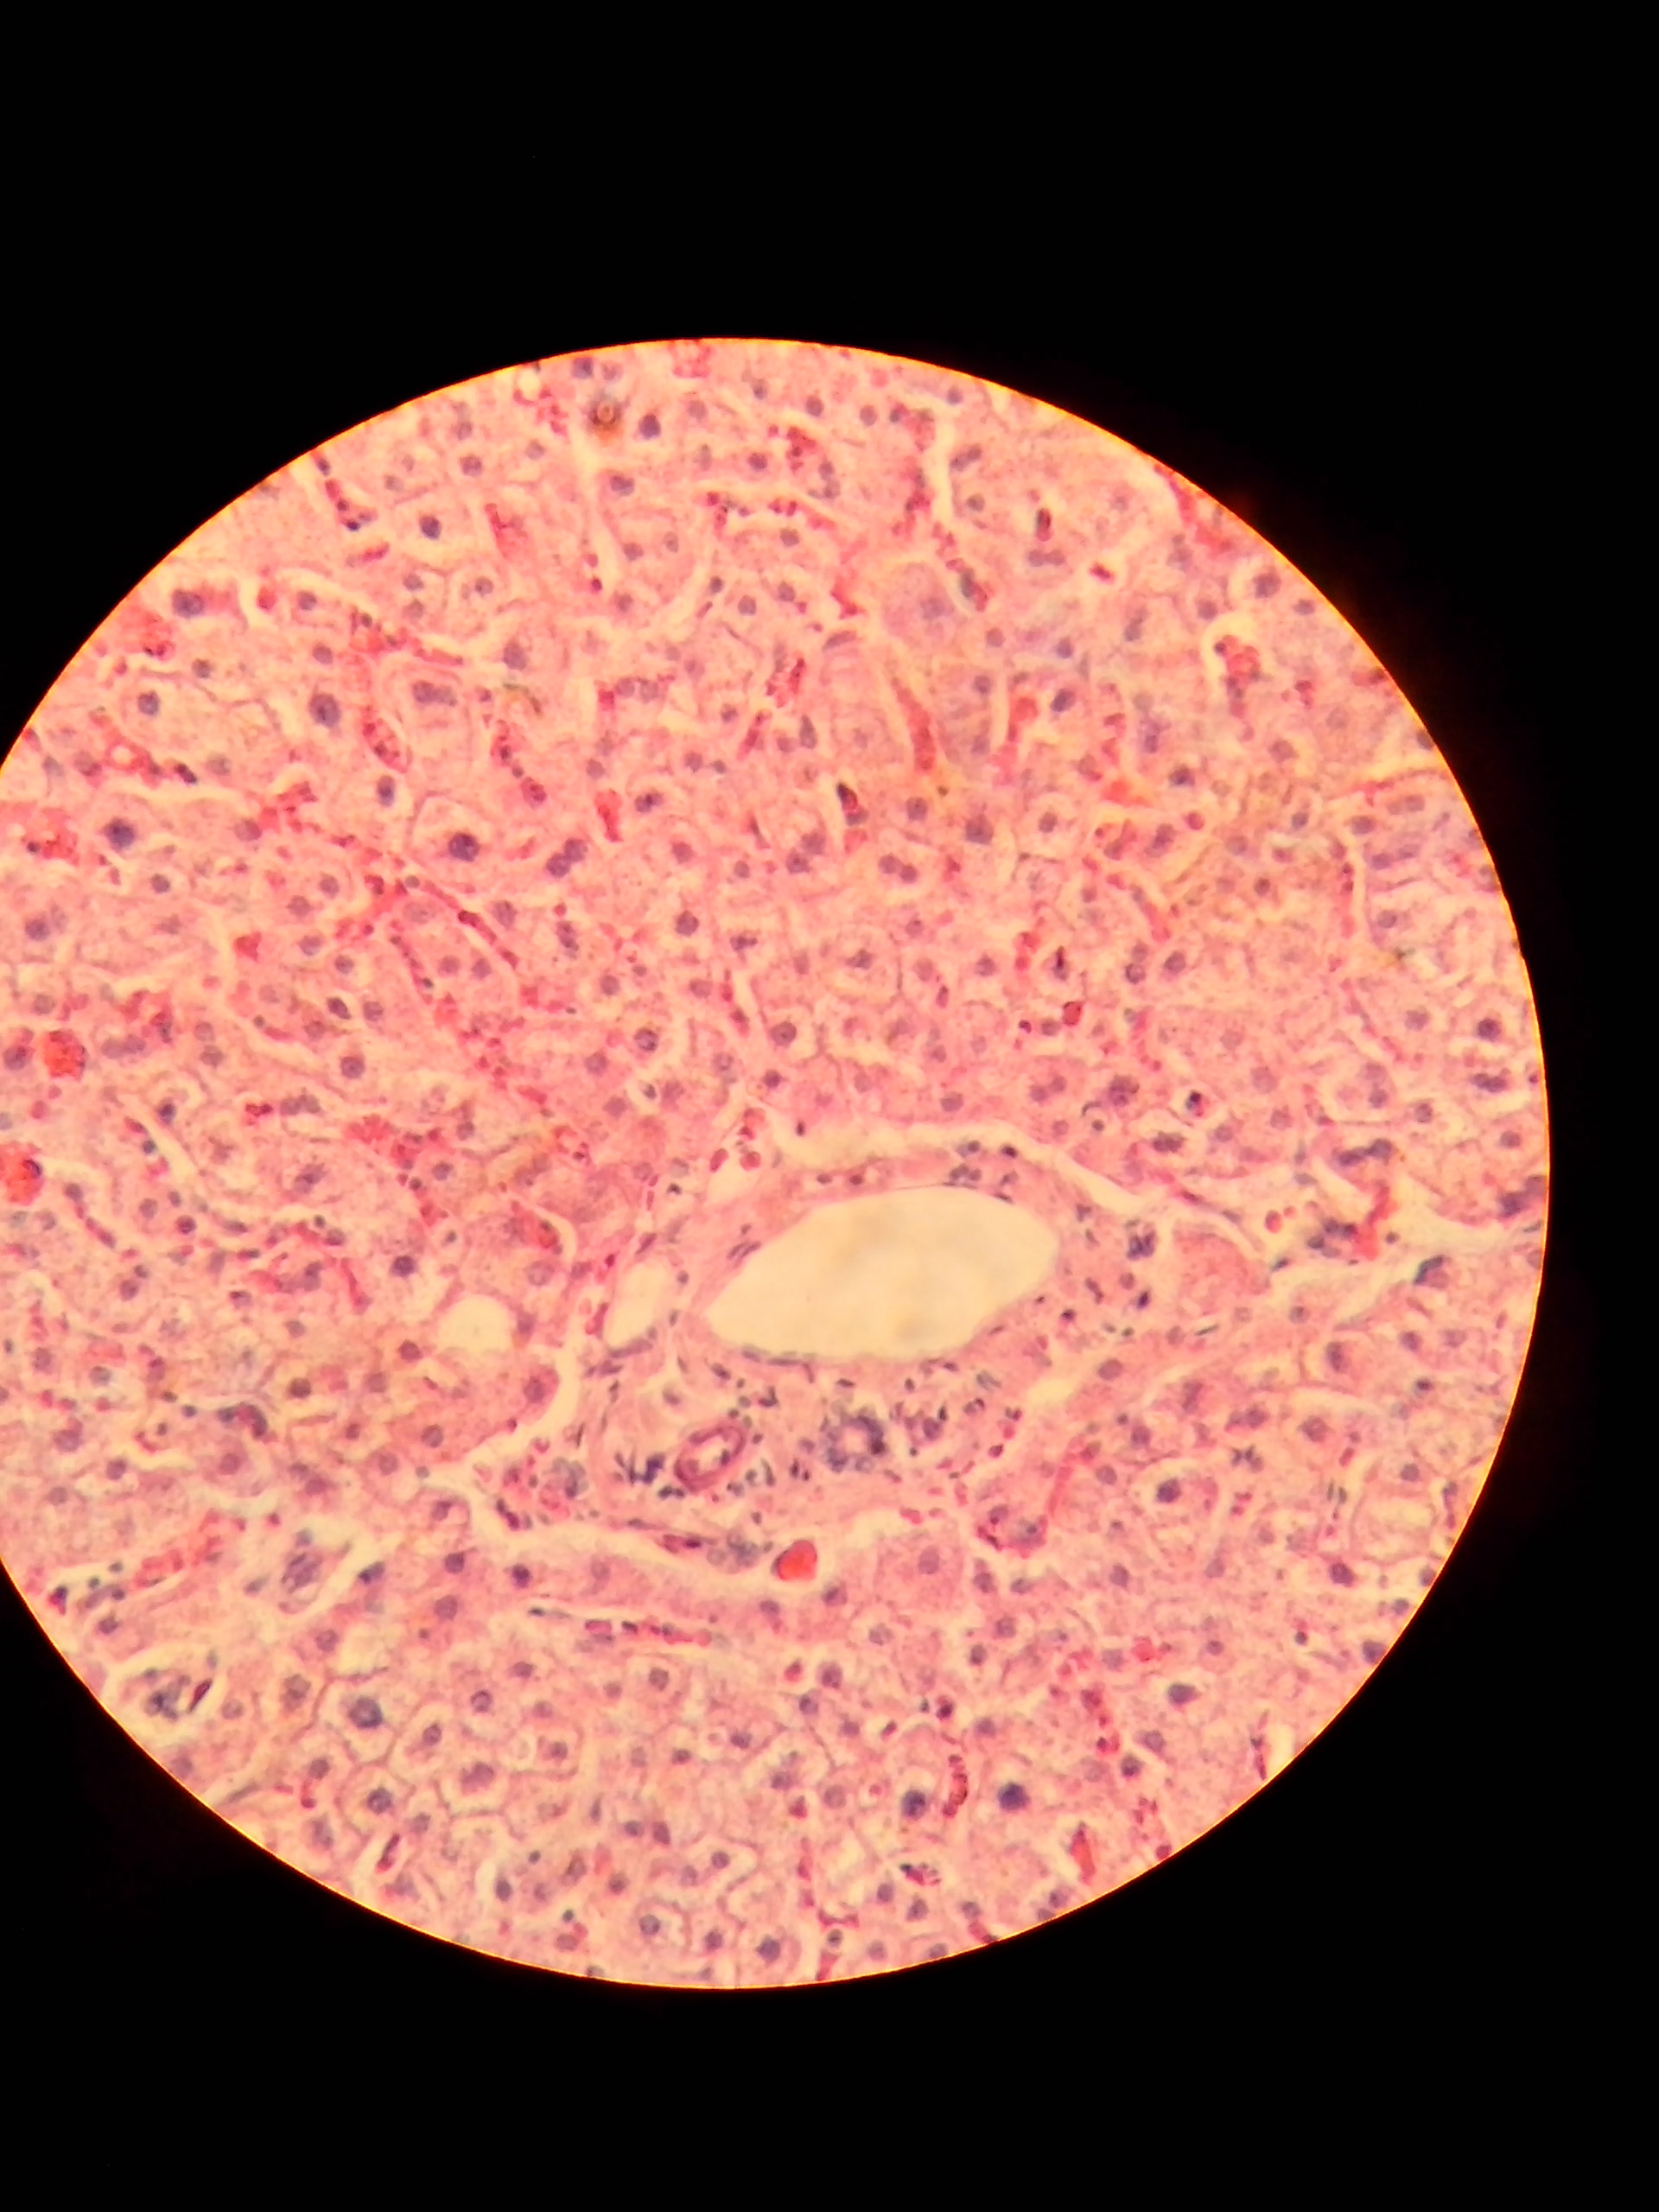
\includegraphics[width=1\textwidth]{../images/08_human_liver.jpg}
		\caption{Gallengefäss -- Objektiv 40x}
		\label{fig:08_human_liver}
	\end{subfigure}
	\begin{subfigure}[b]{0.3\textwidth}
		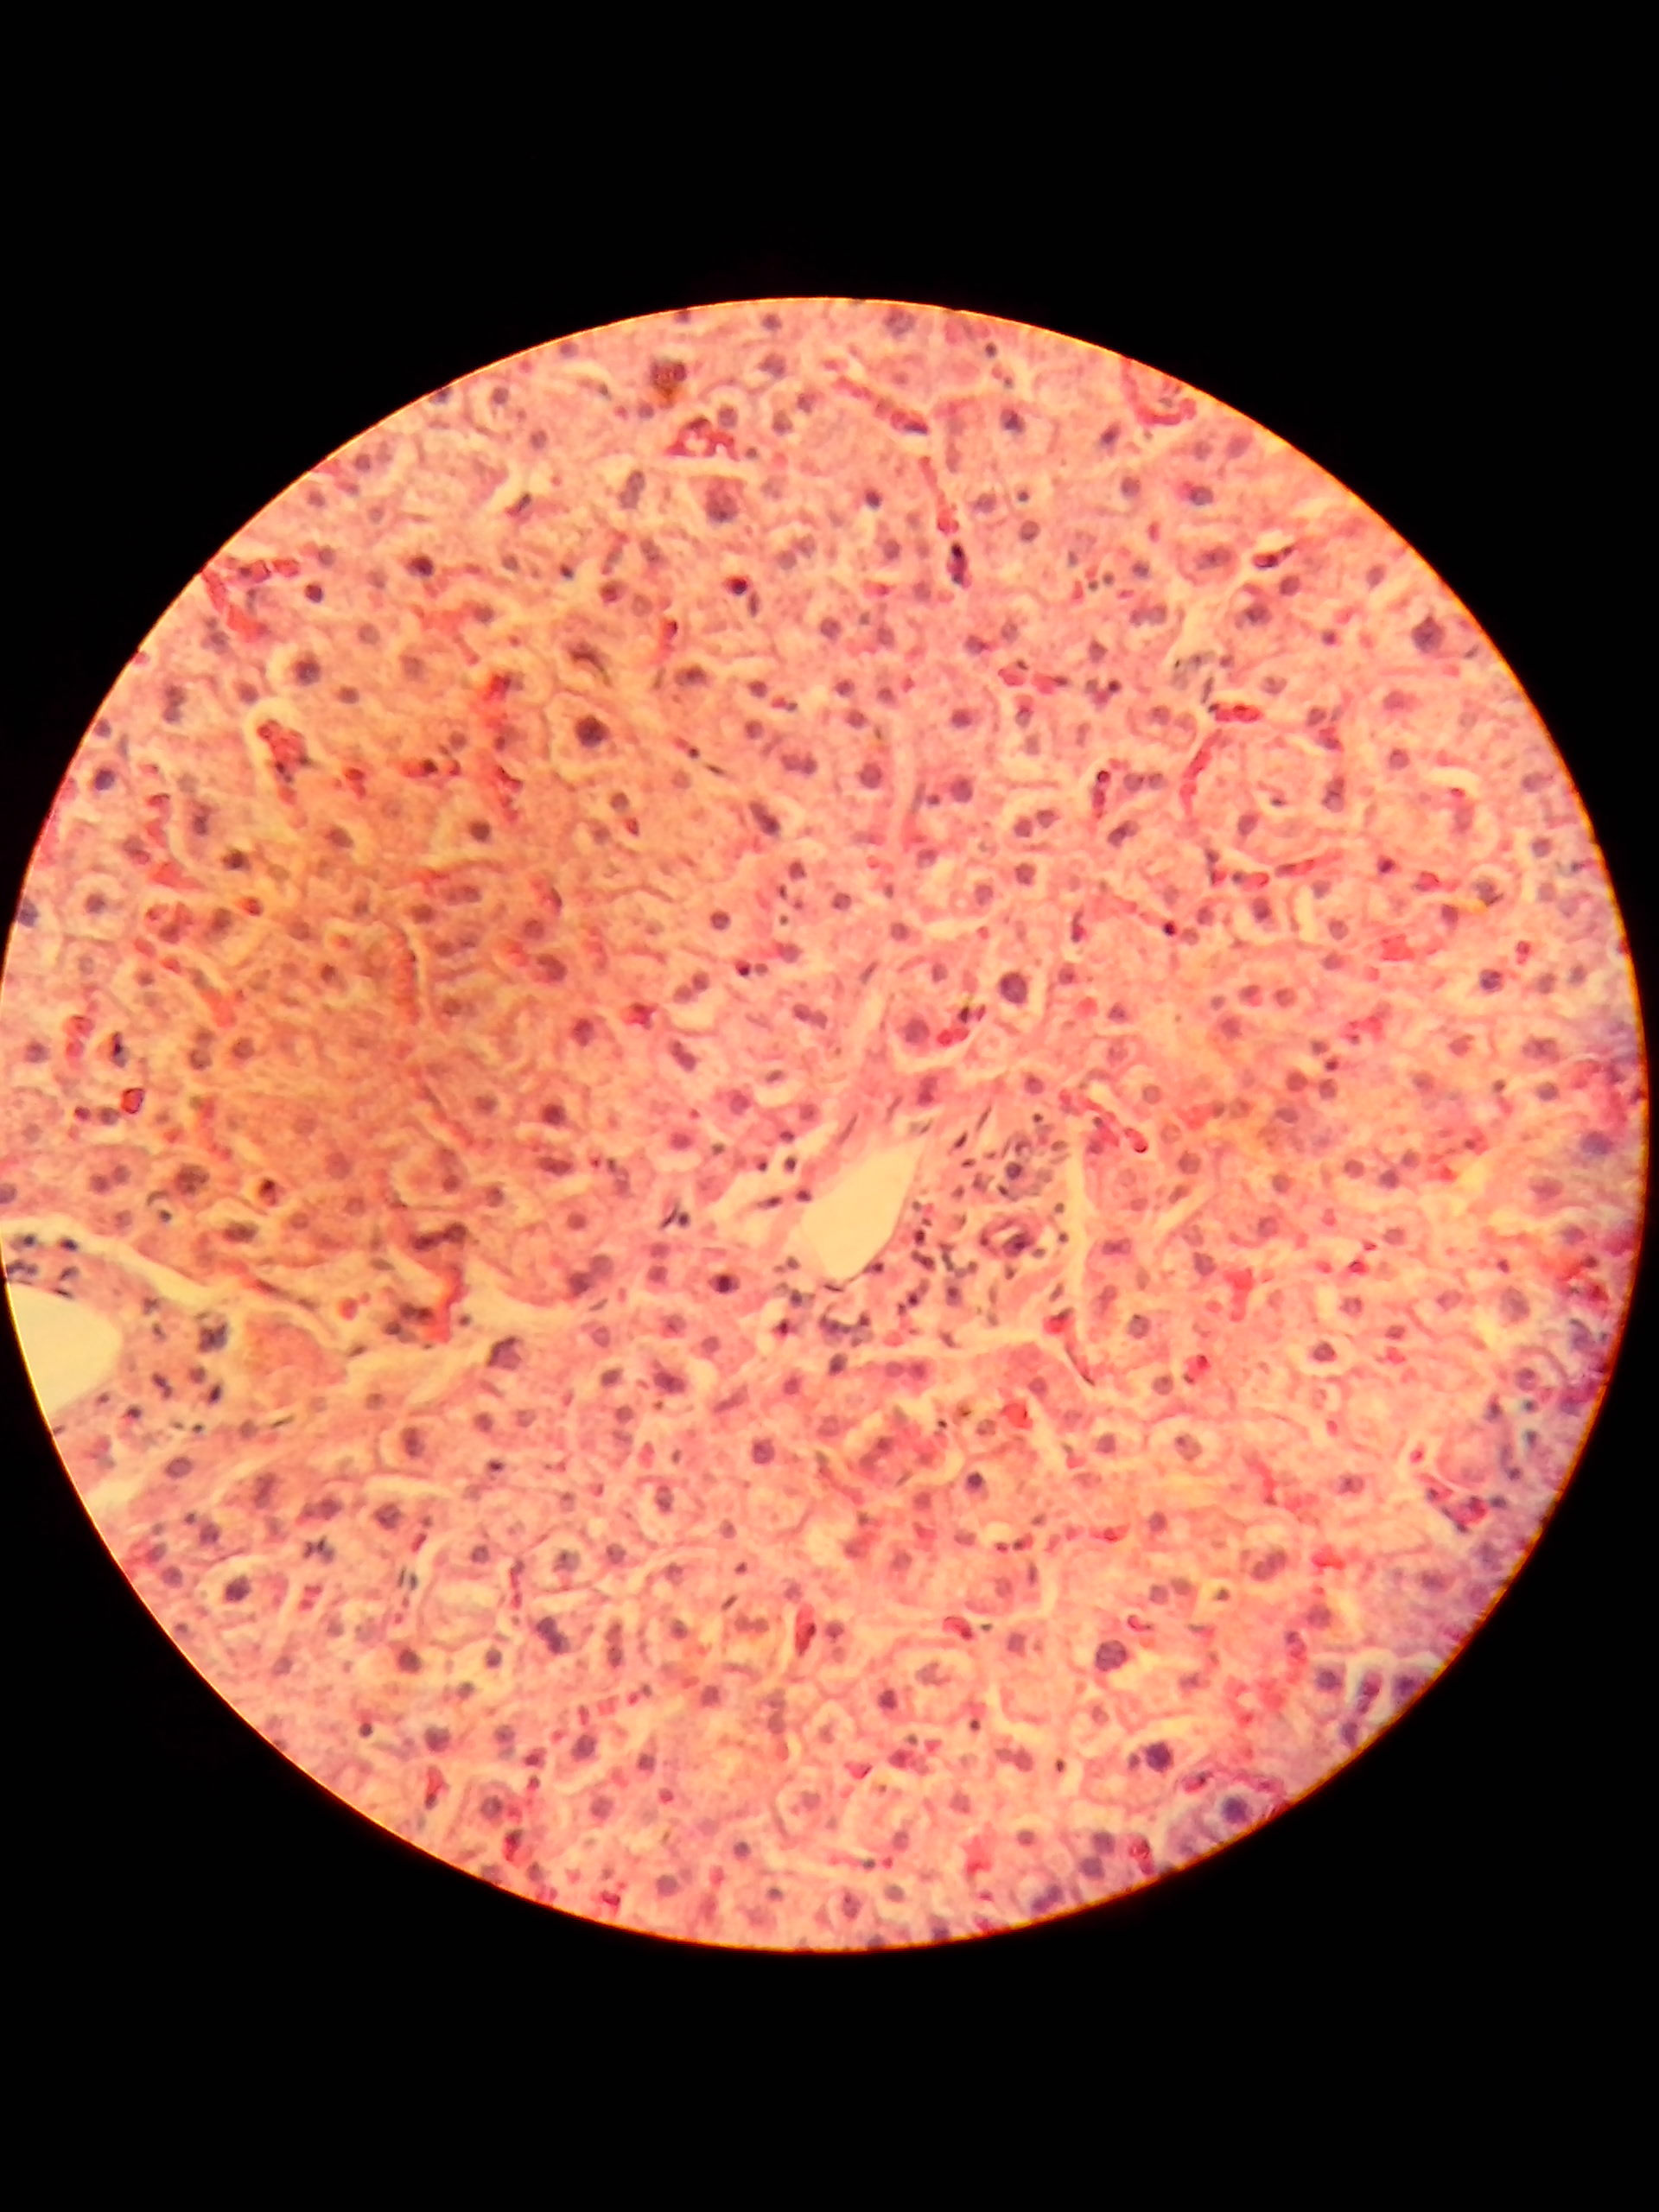
\includegraphics[width=1\textwidth]{../images/10_human_liver.jpg}
		\caption{Arteriengefäss -- Objektiv 40x}
		\label{fig:10_human_liver}
	\end{subfigure}
	\caption{Aufzeichnungen der Lichtmikorskopischen Darstellungen der
		menschlichen Leber}
\end{figure}

\subsubsection{Kommentar}
Das Gewebe der menschlichen Leber ist geprägt durch lokale Gefässgruppen.
Diese treten als Dreiergruppe auf bestehend aus je einem Gefäss der Vene,
Arterie und Galle. Die Durchmesser dieser Gefässe sind wie folgt
\[ 
	\o_{Vene} > \o_{Arterie} > \o_{Galle}
\]
Eine solche Gefässgruppe ist in den Abbildungen \ref{fig:01_human_liver}
bis \ref{fig:05_human_liver} dargestellt. In den gezeigten Abbildungen
sind die Grössenunterschiede der Gefässdurchmesser deutlich zu erkennen.
Die Abbildungen \ref{fig:07_human_liver} bis \ref{fig:10_human_liver}
zeigen die verschiedenen Gefässe nochmals in höherer Auflösung jeweils
mit dem selben Objektiv bzw. mit der selben Vergrösserung.

\newpage
\subsection{Menschliche Bauchspeicheldrüse}

\subsubsection{Proben}
\begin{table}[h!]
	\centering
	\begin{tabular}{l l}
		Bezeichnung	& Pankreas \\
		Probe 		& 31-5442
	\end{tabular}
\end{table}

\subsubsection{Aufzeichnungen}
\begin{figure}[h!]
	\centering
	\begin{subfigure}[b]{0.3\textwidth}
		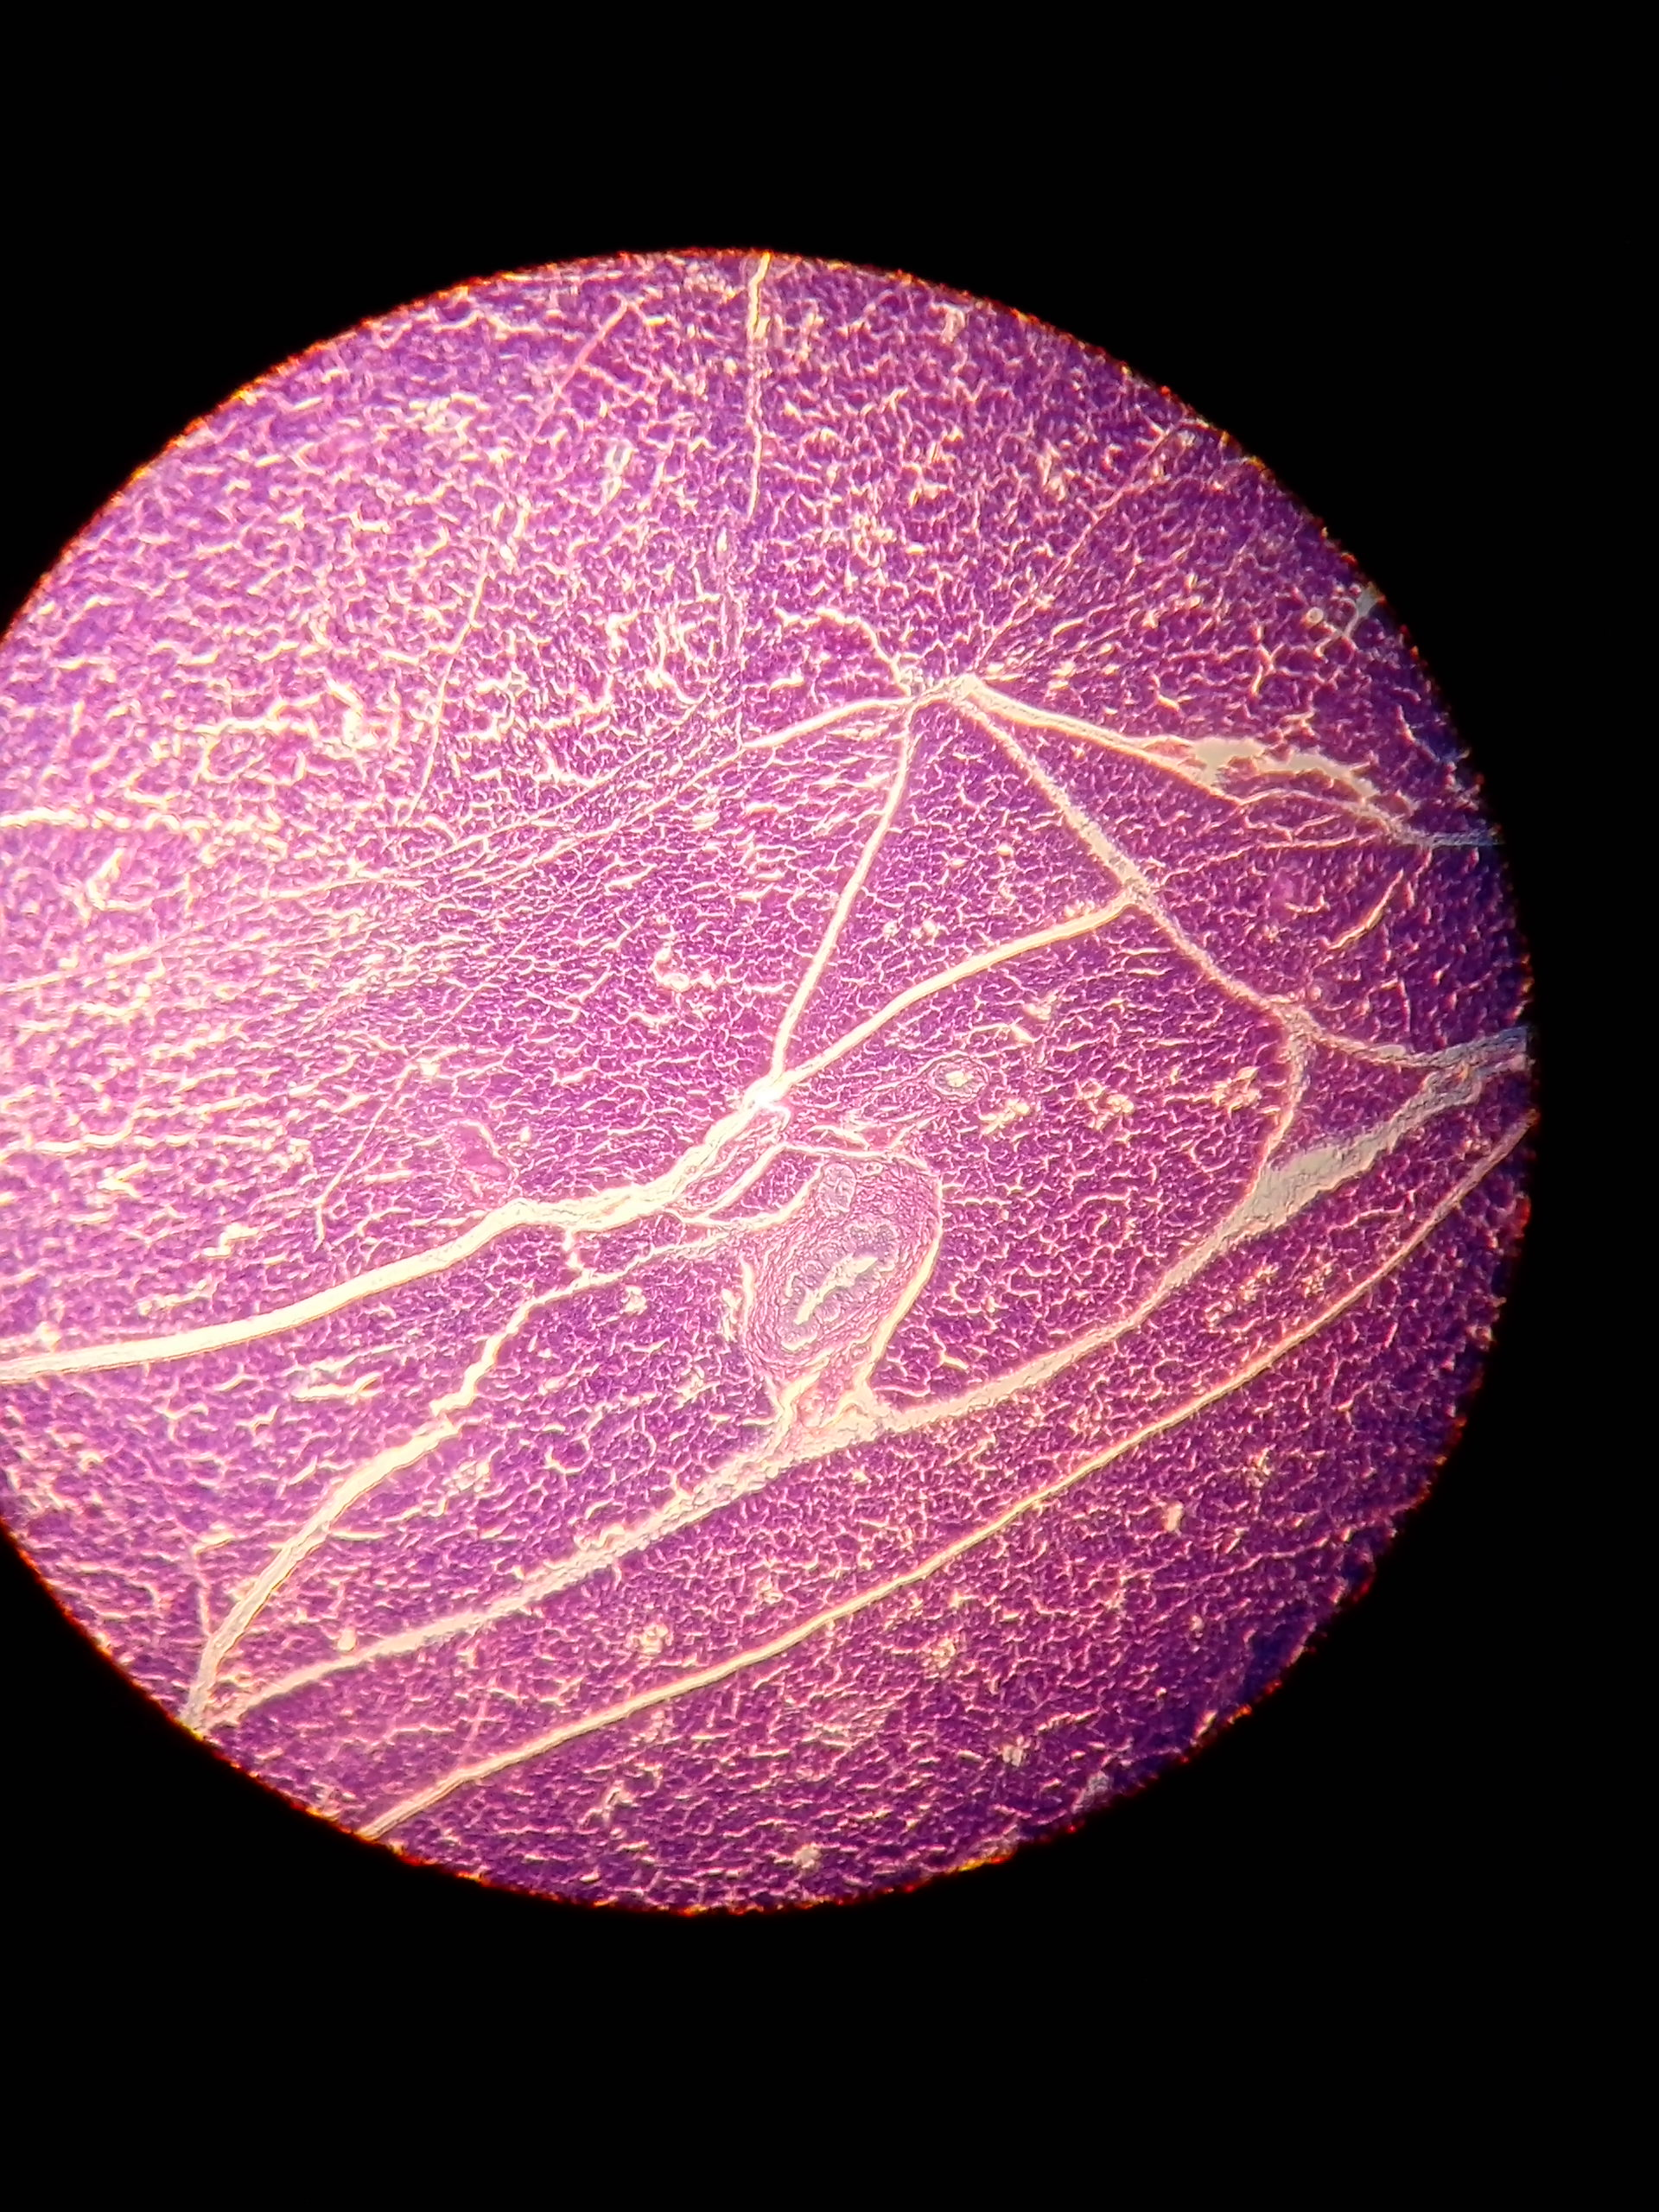
\includegraphics[width=1\textwidth]{../images/01_pankreas.jpg}
		\caption{Objektiv 10x}
		\label{fig:01_pankreas}
	\end{subfigure}
	\begin{subfigure}[b]{0.3\textwidth}
		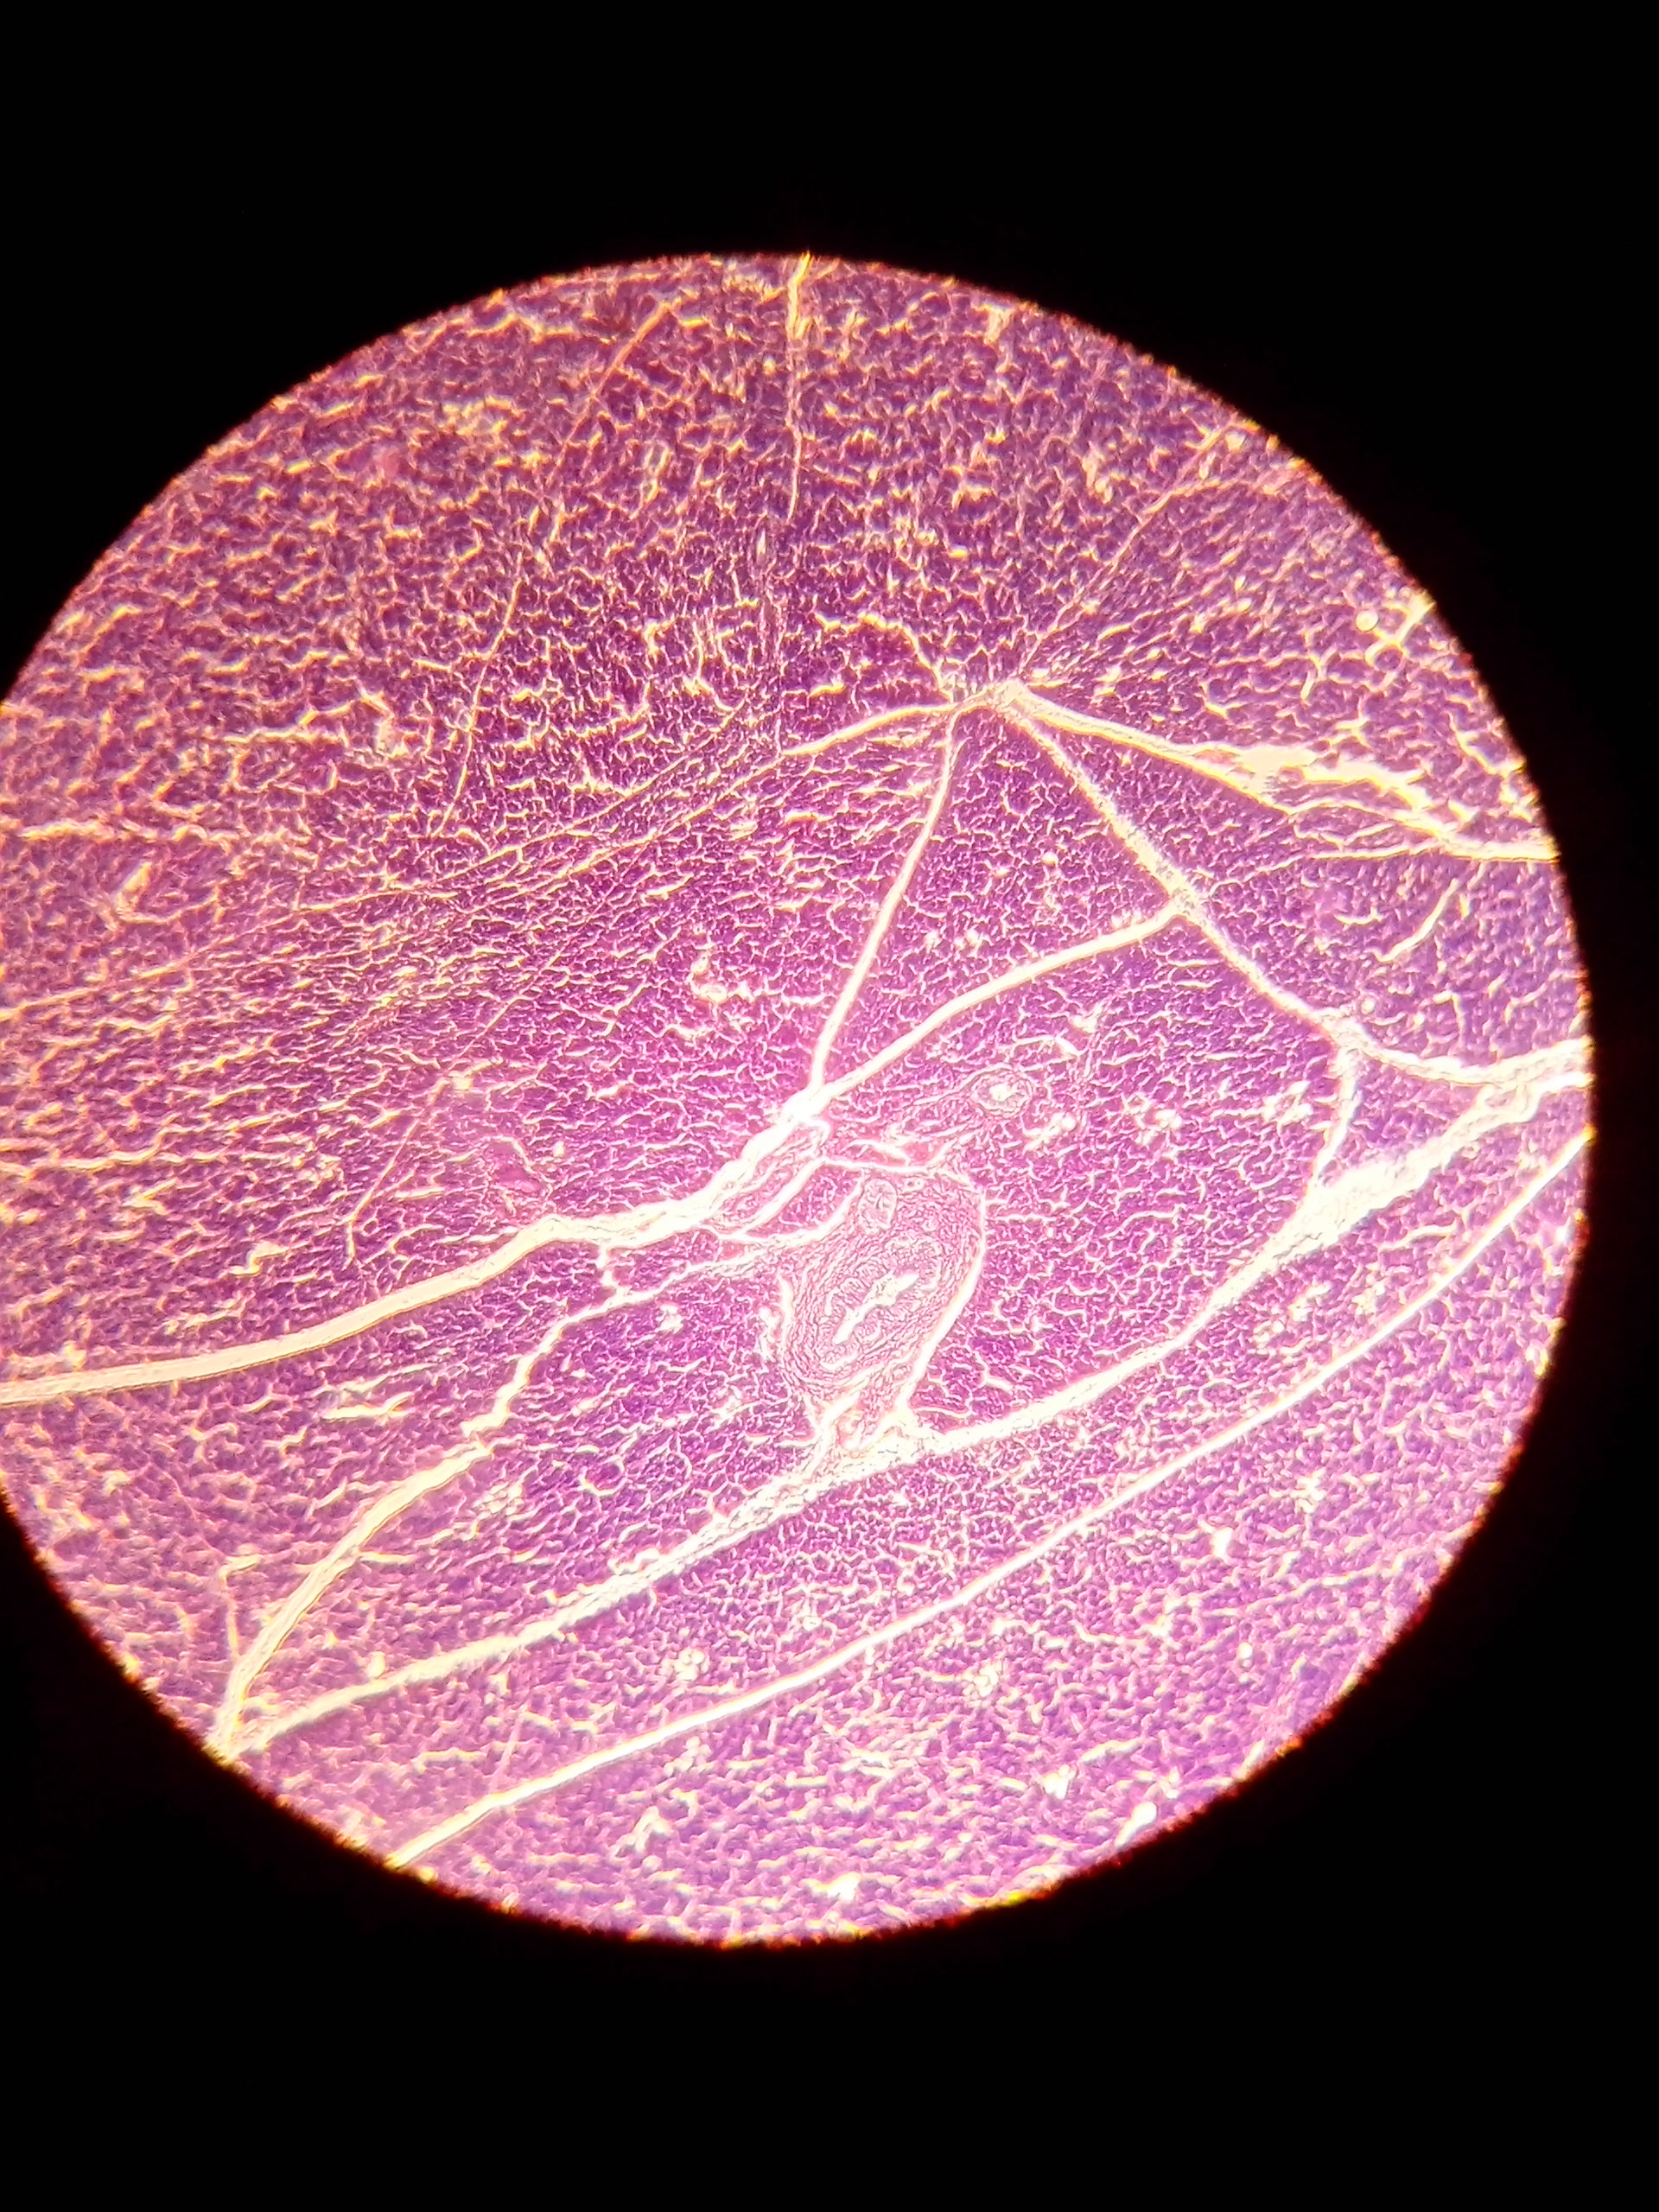
\includegraphics[width=1\textwidth]{../images/02_pankreas.jpg}
		\caption{Objektiv 10x}
		\label{fig:02_pankreas}
	\end{subfigure}

	\begin{subfigure}[b]{0.3\textwidth}
		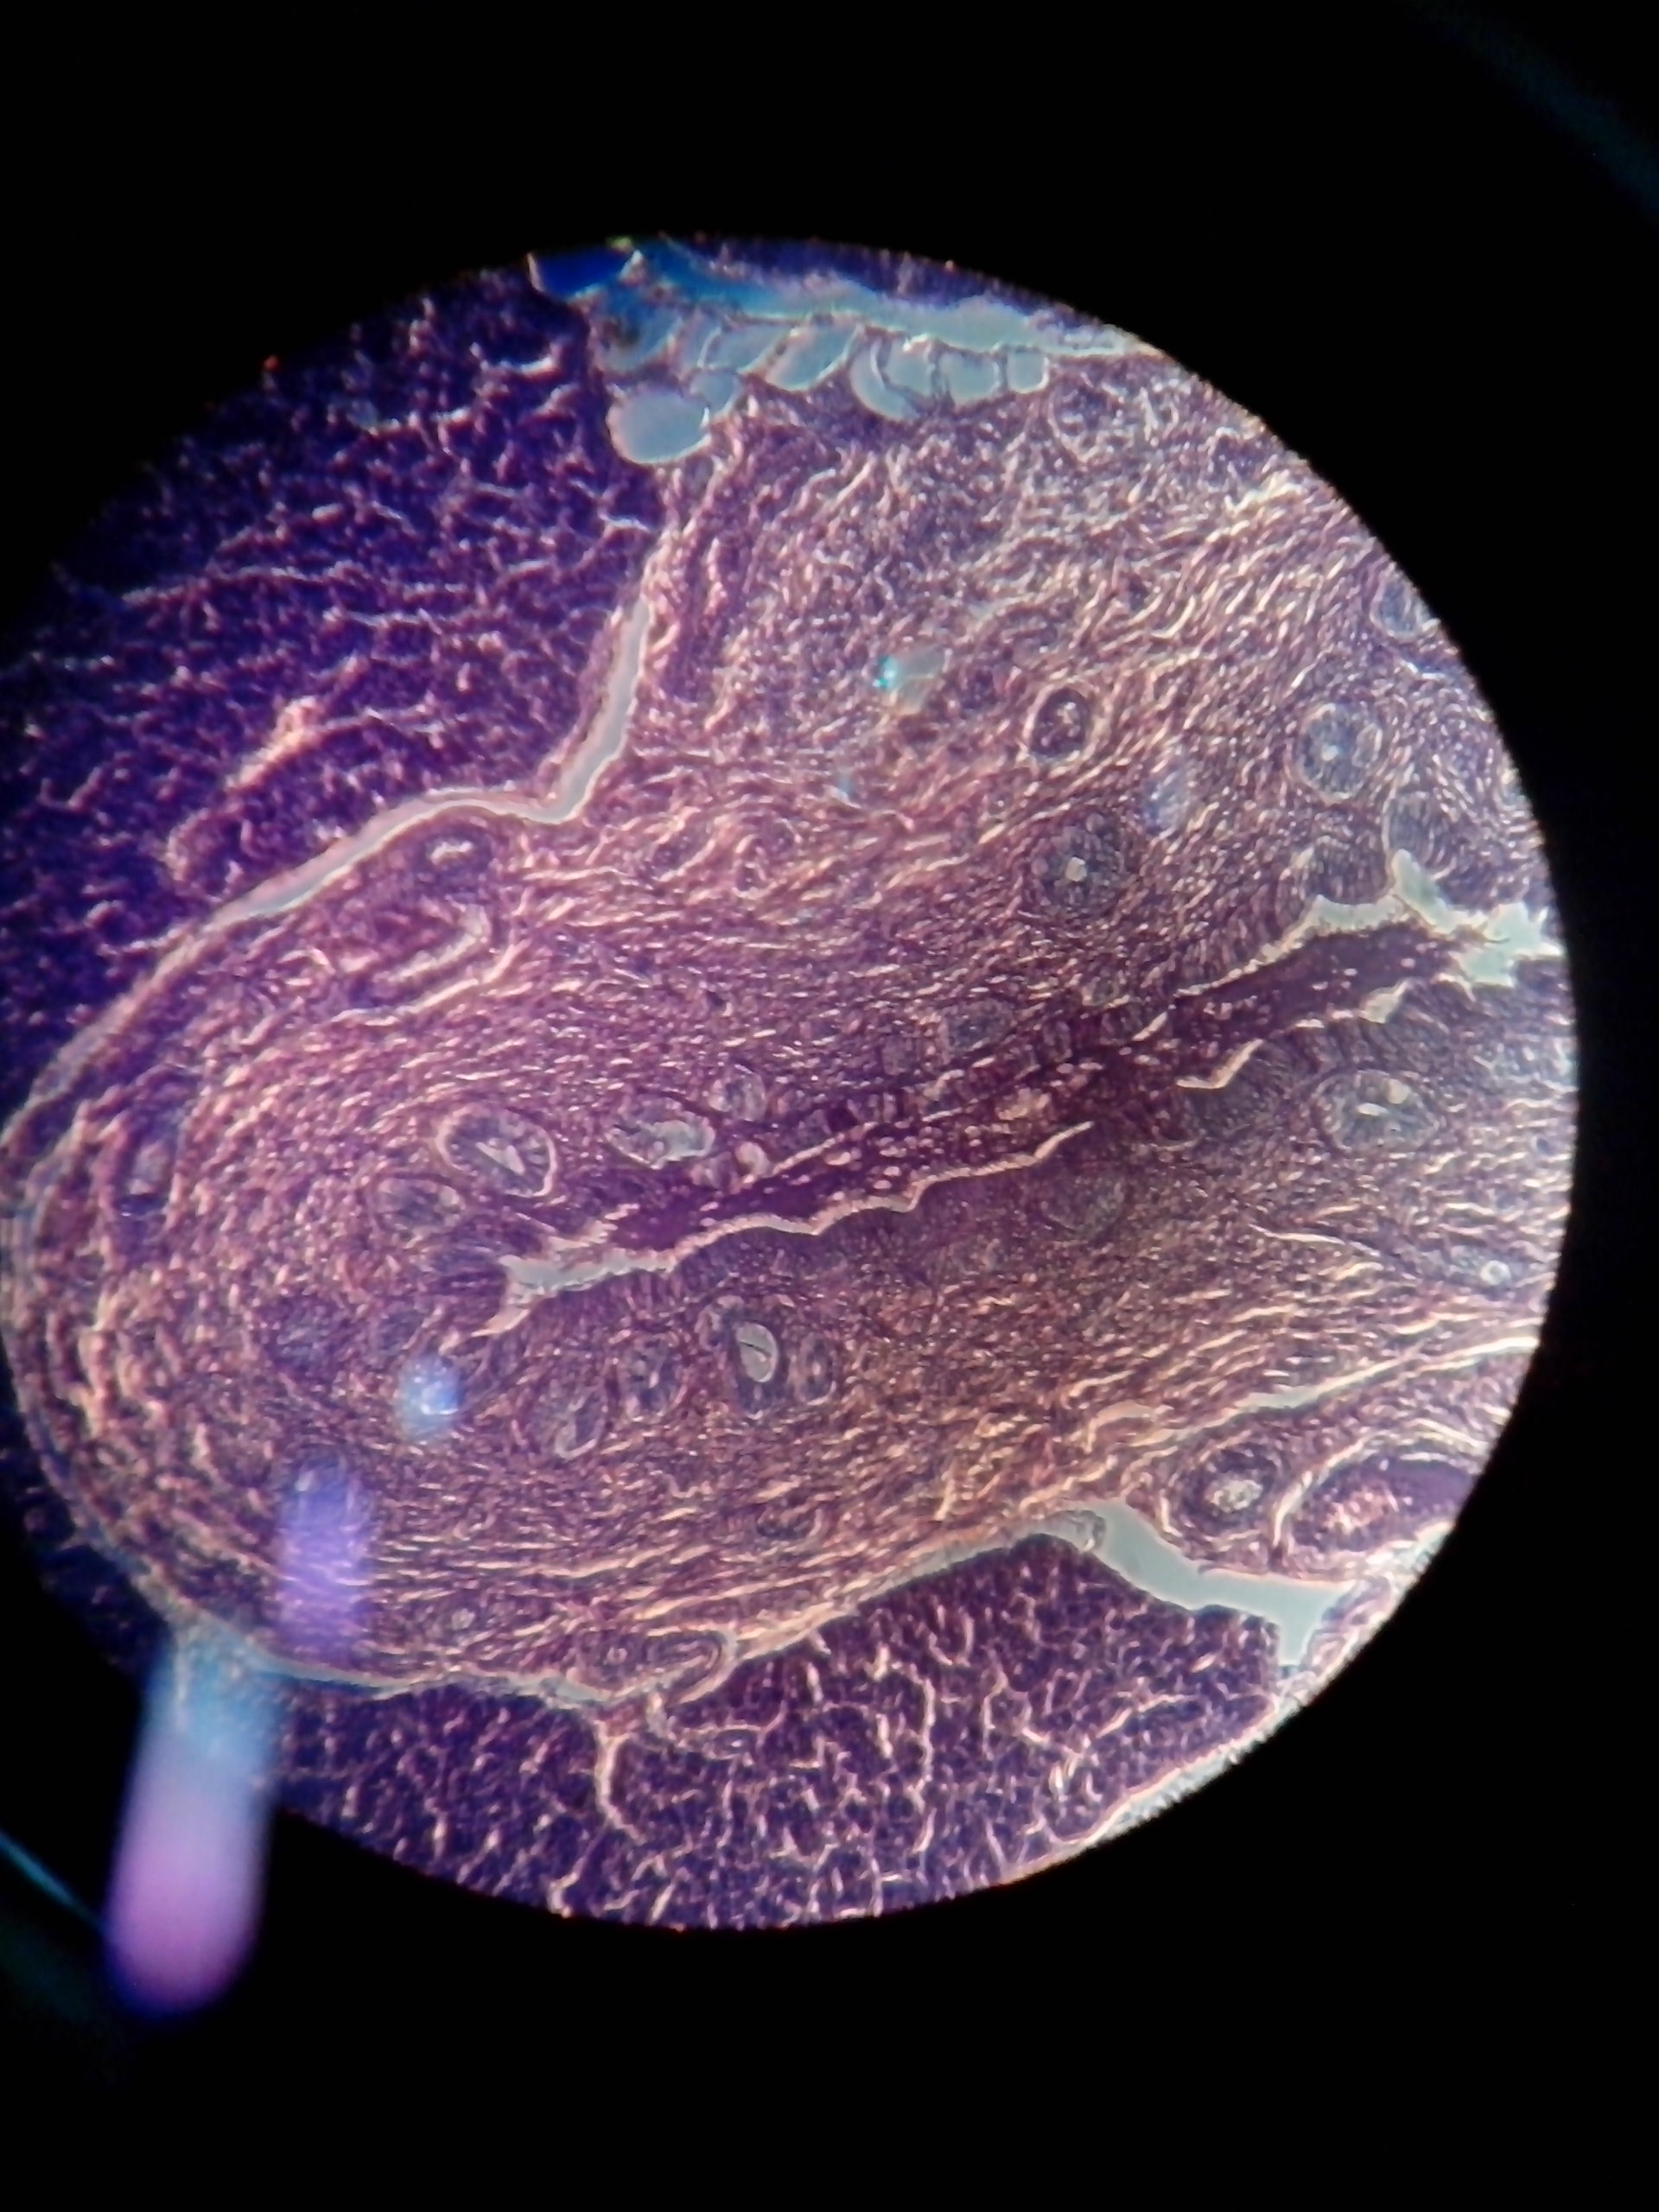
\includegraphics[width=1\textwidth]{../images/03_pankreas.jpg}
		\caption{Objektiv 20x}
		\label{fig:03_pankreas}
	\end{subfigure}
	\begin{subfigure}[b]{0.3\textwidth}
		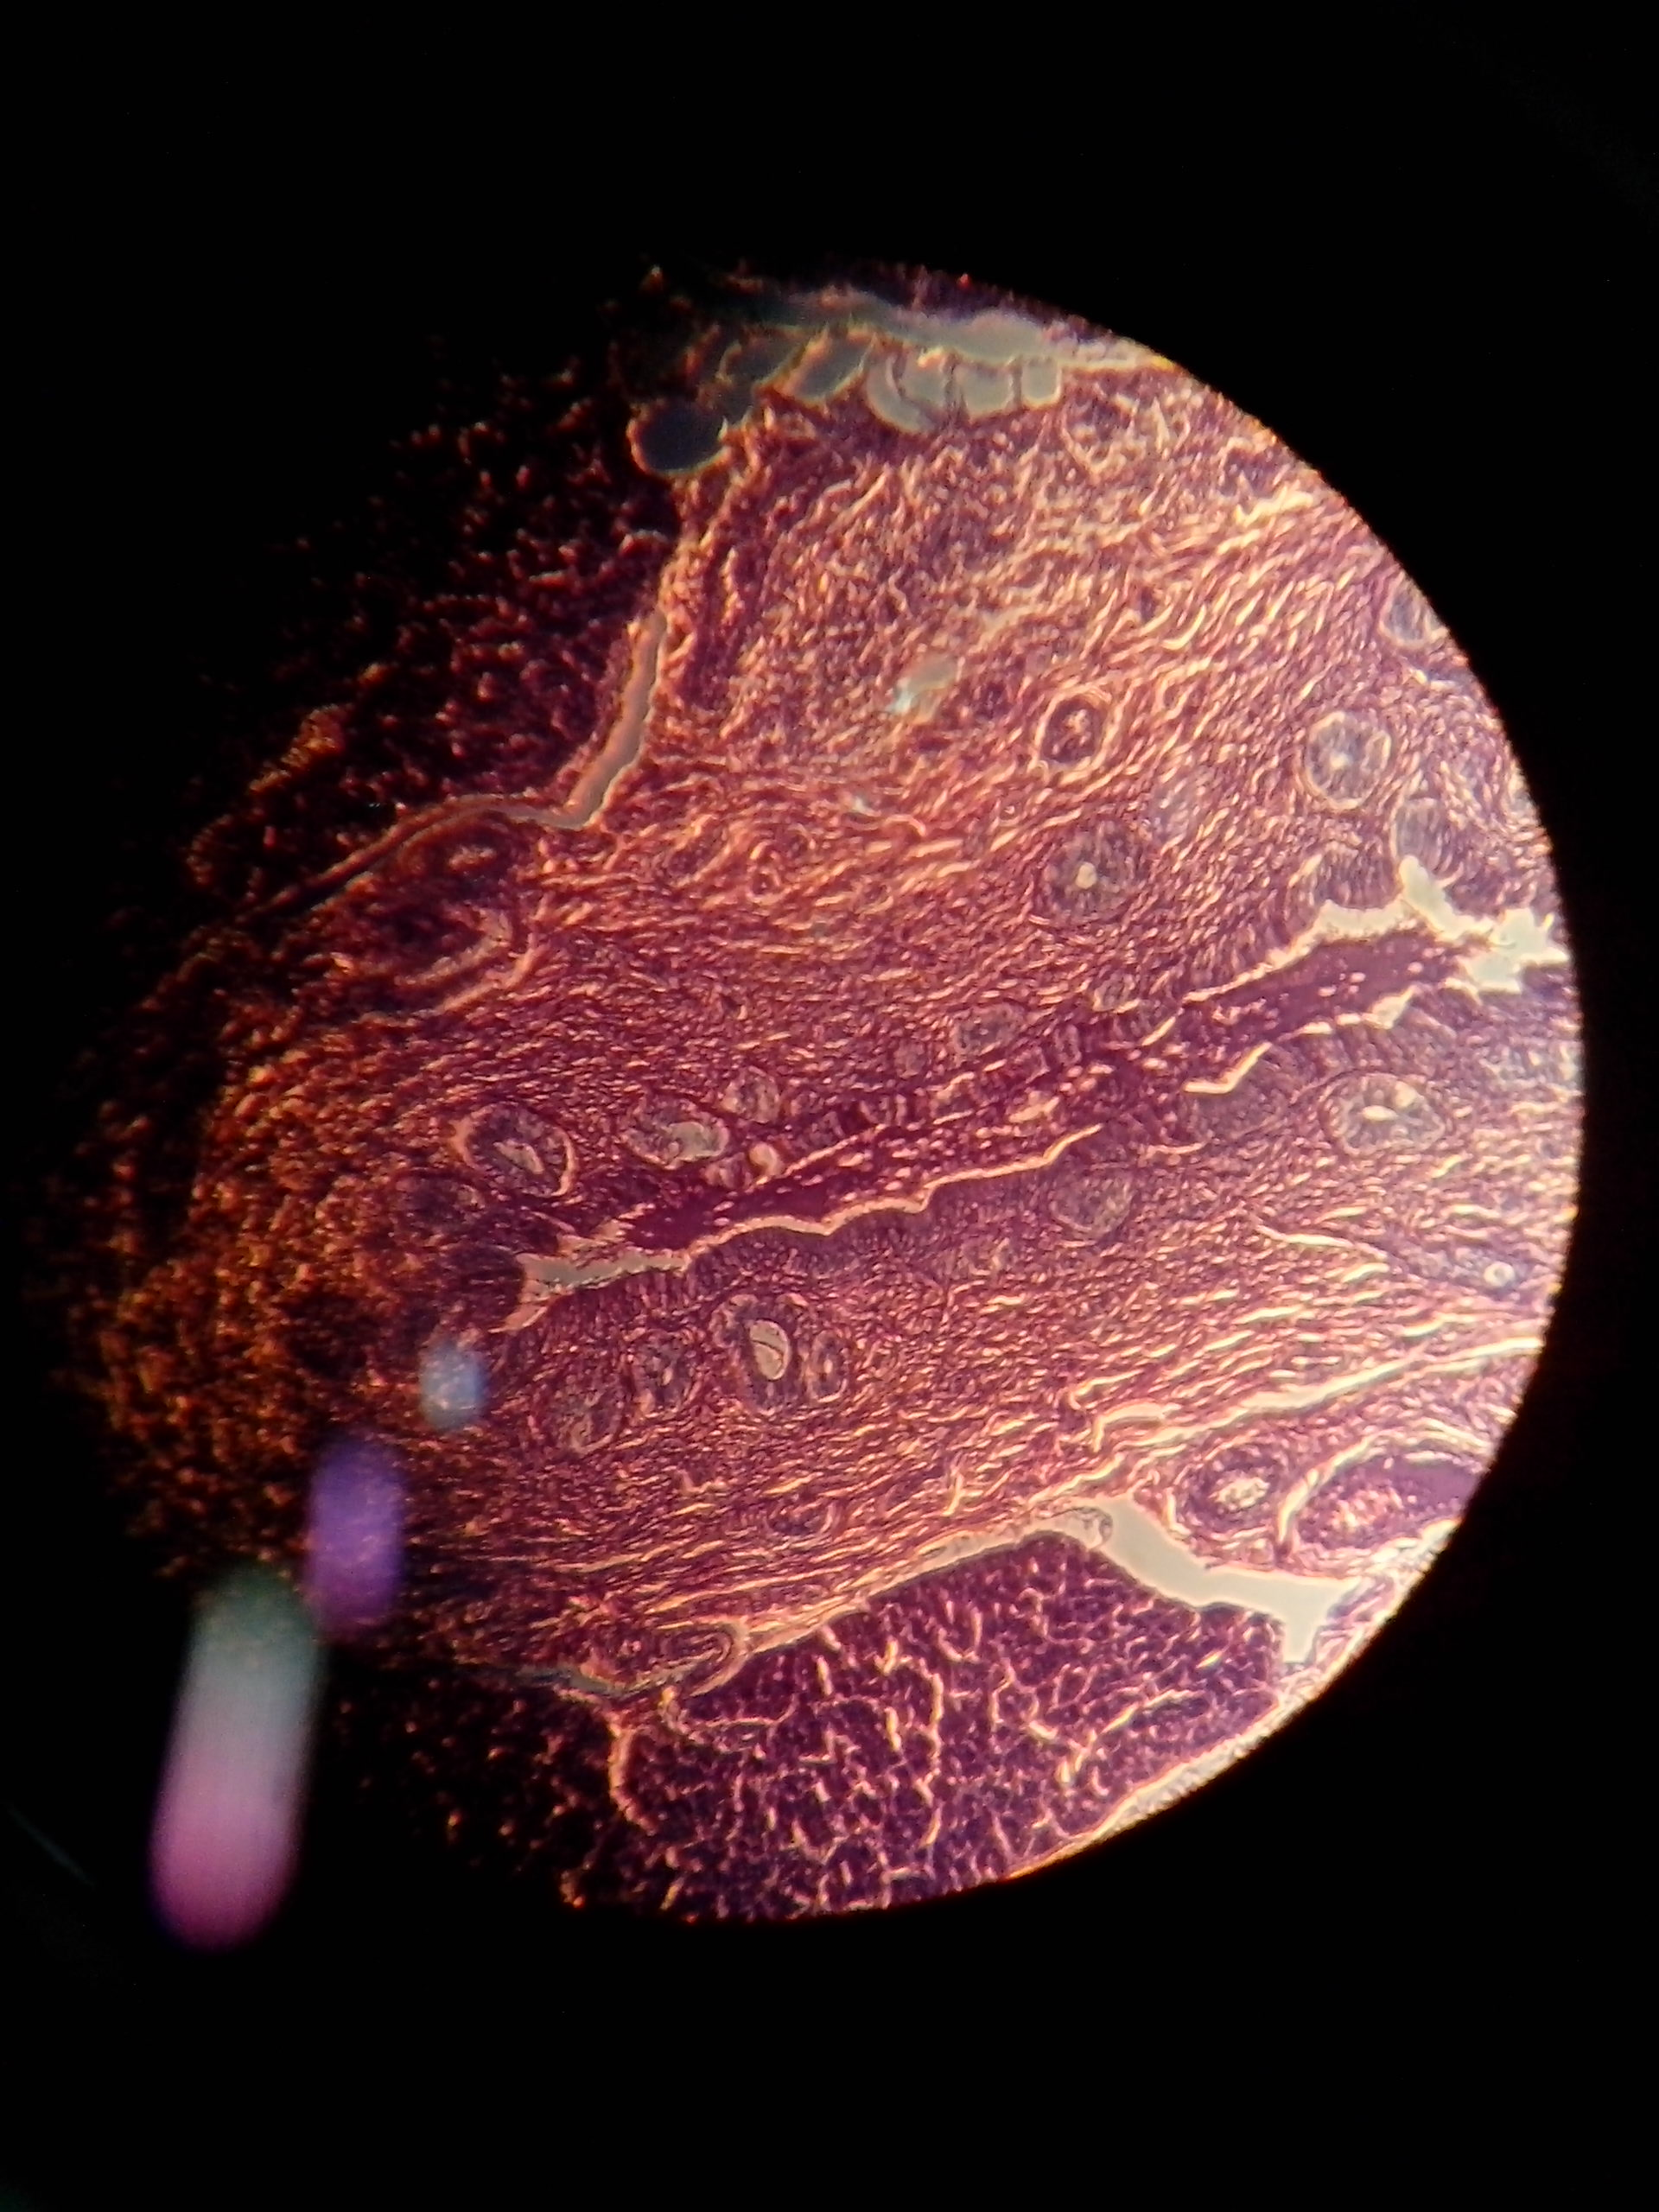
\includegraphics[width=1\textwidth]{../images/04_pankreas.jpg}
		\caption{Objektiv 20x}
		\label{fig:04_pankreas}
	\end{subfigure}
	\caption{Aufzeichnungen der Lichtmikorskopischen Darstellungen der
		menschlichen Bauchspeicheldrüse}
\end{figure}

\subsubsection{Kommentar}
Das Gewebe der menschlichen Bauchspeicheldrüse, auch Pankreas genannt,
beinhaltet lokal begrenzte Gewebestrukturen die sich in ihrem Kontrast vom
umgebenden Gewebe unterscheiden. Unter dem Mikroskop erscheint dieses Gewebe
in der eingefärbten Gewebeprobe der menschlichen Bauchspeichedrüse heller als
das Restgewebe. Dies ist in den Abbildungen \ref{fig:01_pankreas} und
\ref{fig:02_pankreas} dargestellt. Diese Gewebegruppe bildet eine sogenannte
exokrine Drüse\footnote{Exokrine Drüsen geben Produkte in Körperhohlräume ab.
Im Gegensatz zu den exokrinen Drüsen geben endokrine Drüsen ihre Produkte
direkt ins Blut ab.} welche als Inselapparat bezeichnet wird. Die selbige ist
in den Abbildungen \ref{fig:03_pankreas} und \ref{fig:04_pankreas} vergrössert
dargestellt.

Diese Inselapparate, auch Langerhans-Inseln genannt, haben auch endokrine
Funktionen. Diese sind für die Hormonproduktion bzw. deren Abgabe ins Blut
verantwortlich \cite{doccheck}.

\newpage
\subsection{Menschlicher Magen}

\subsubsection{Proben}
\begin{table}[h!]
	\centering
	\begin{tabular}{l l}
		Bezeichnung	& human stomach \\
		Probe 		& 31-5100
	\end{tabular}
\end{table}

\subsubsection{Aufzeichnungen}
\begin{figure}[h!]
	\centering
	\begin{subfigure}[b]{0.3\textwidth}
		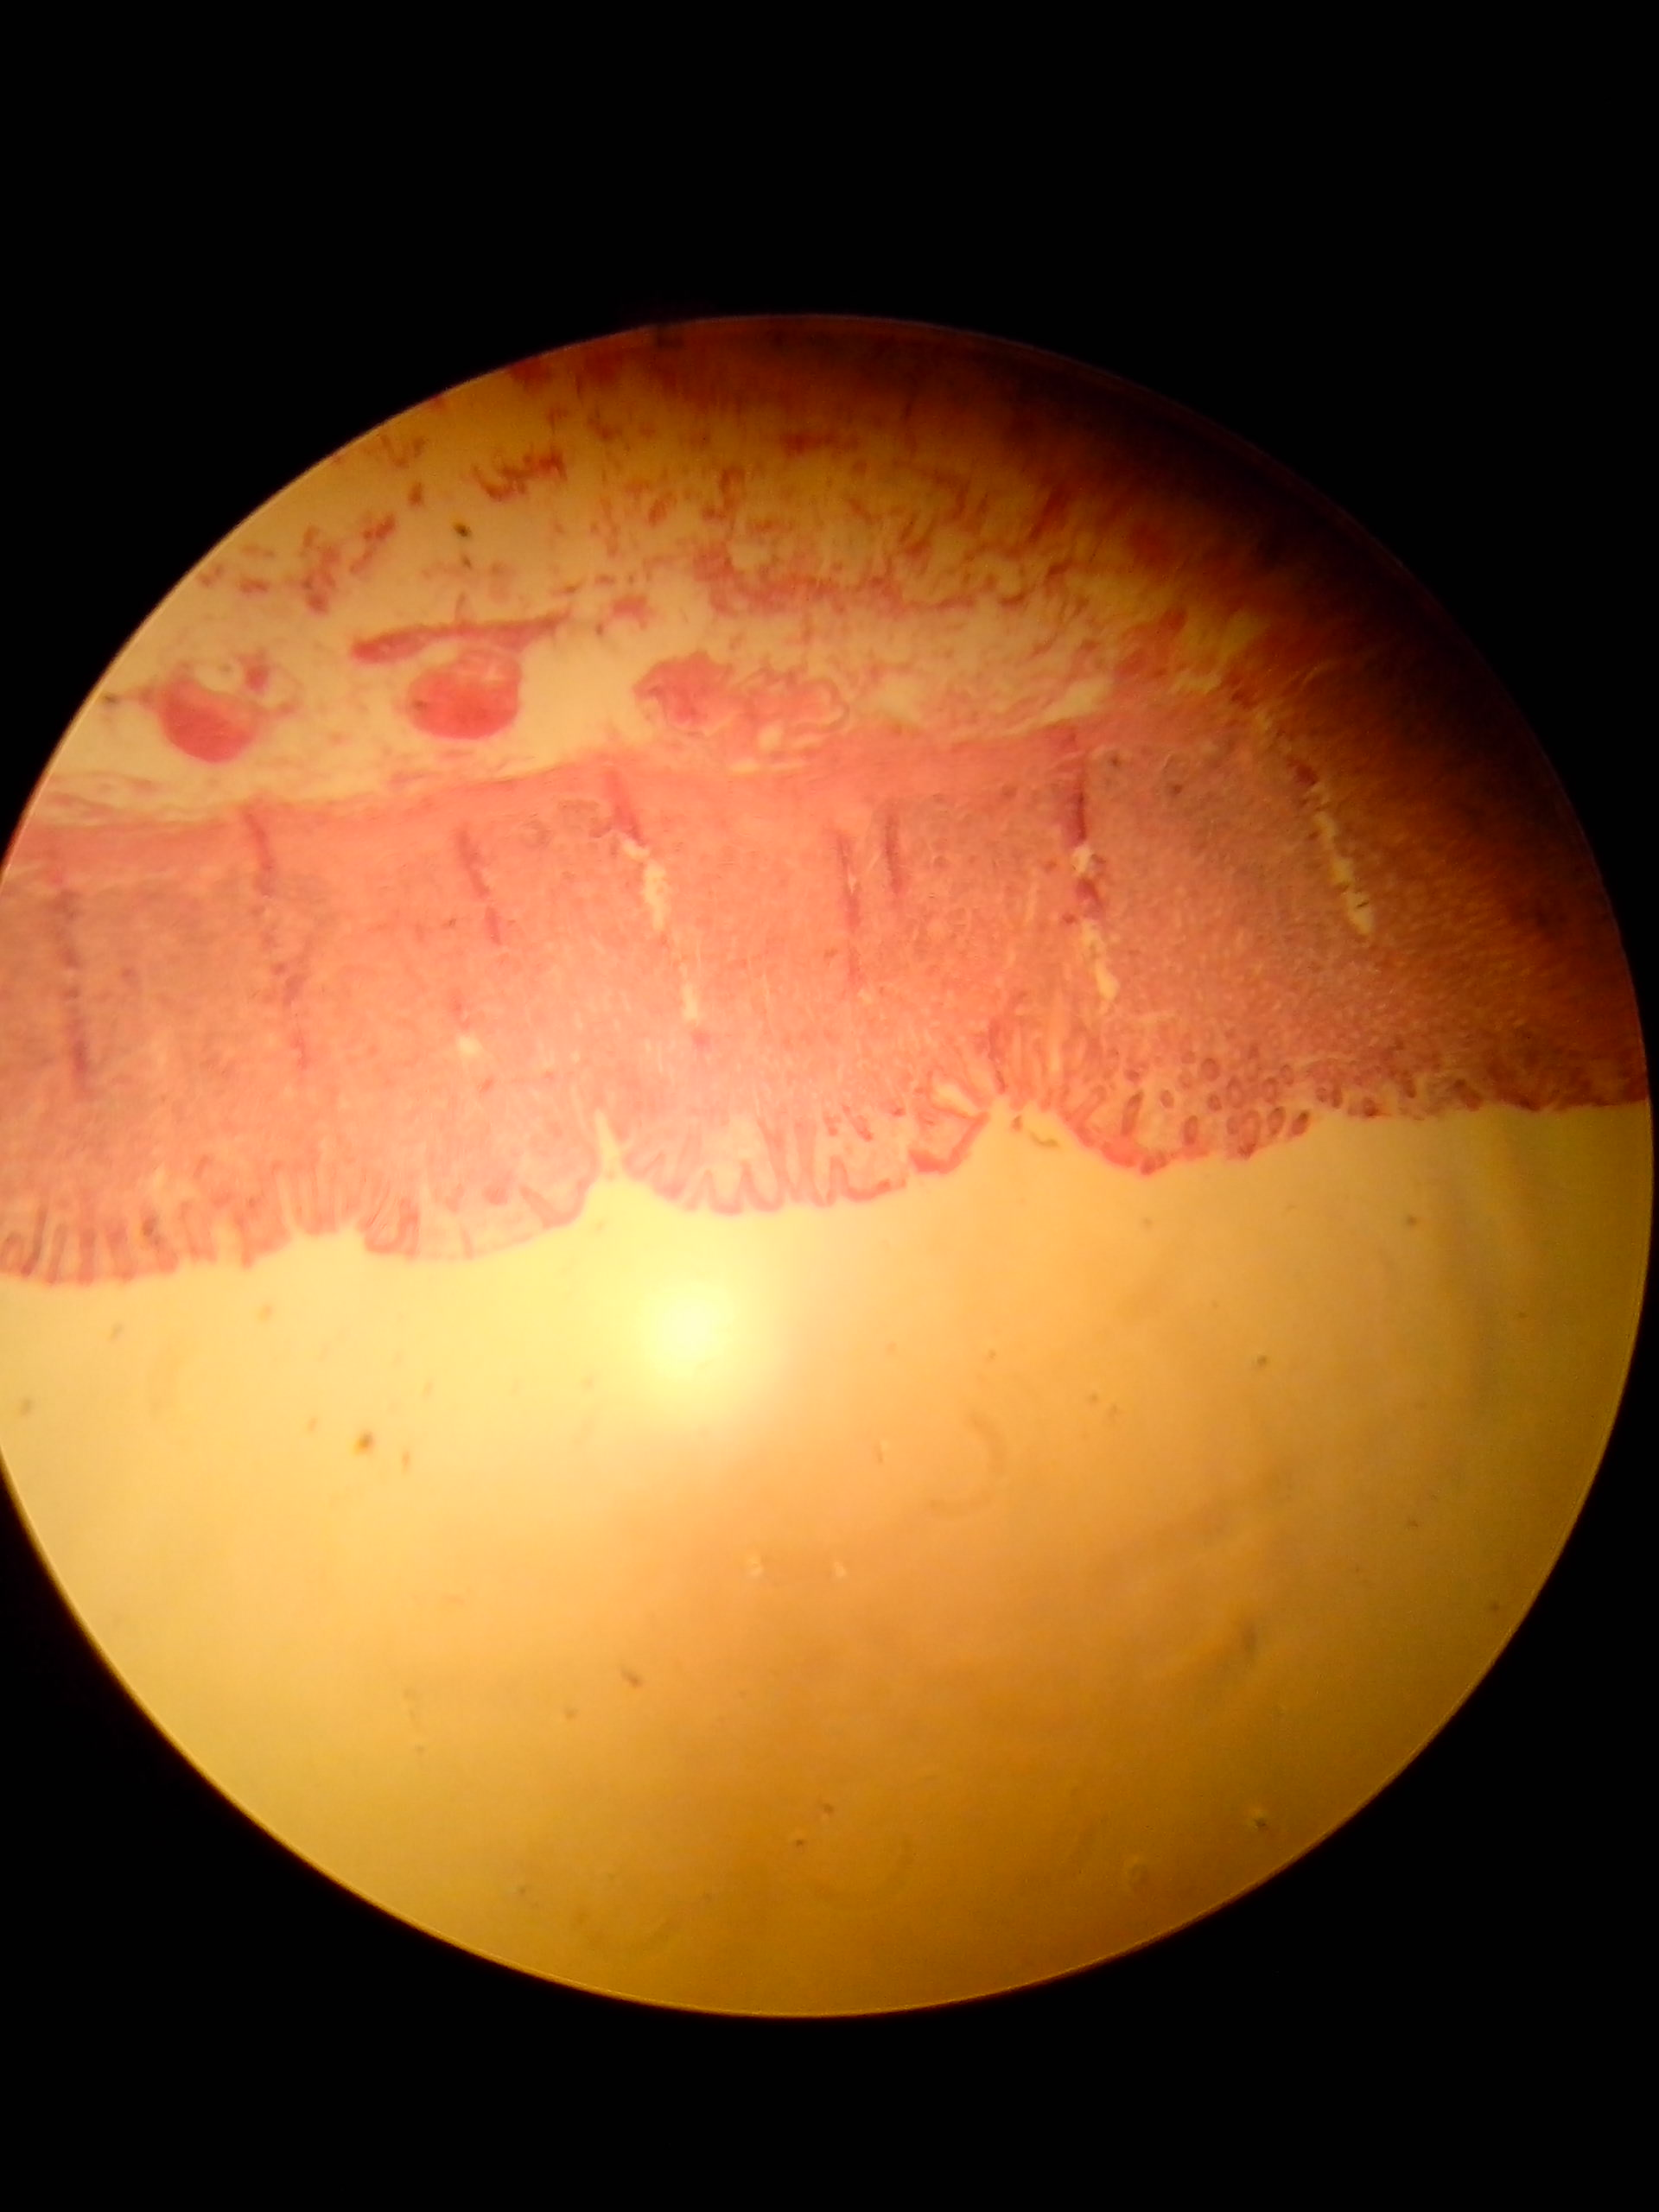
\includegraphics[width=1\textwidth]{../images/01_stomach.jpg}
		\caption{Objektiv 4x}
		\label{fig:01_stomach}
	\end{subfigure}
	\begin{subfigure}[b]{0.3\textwidth}
		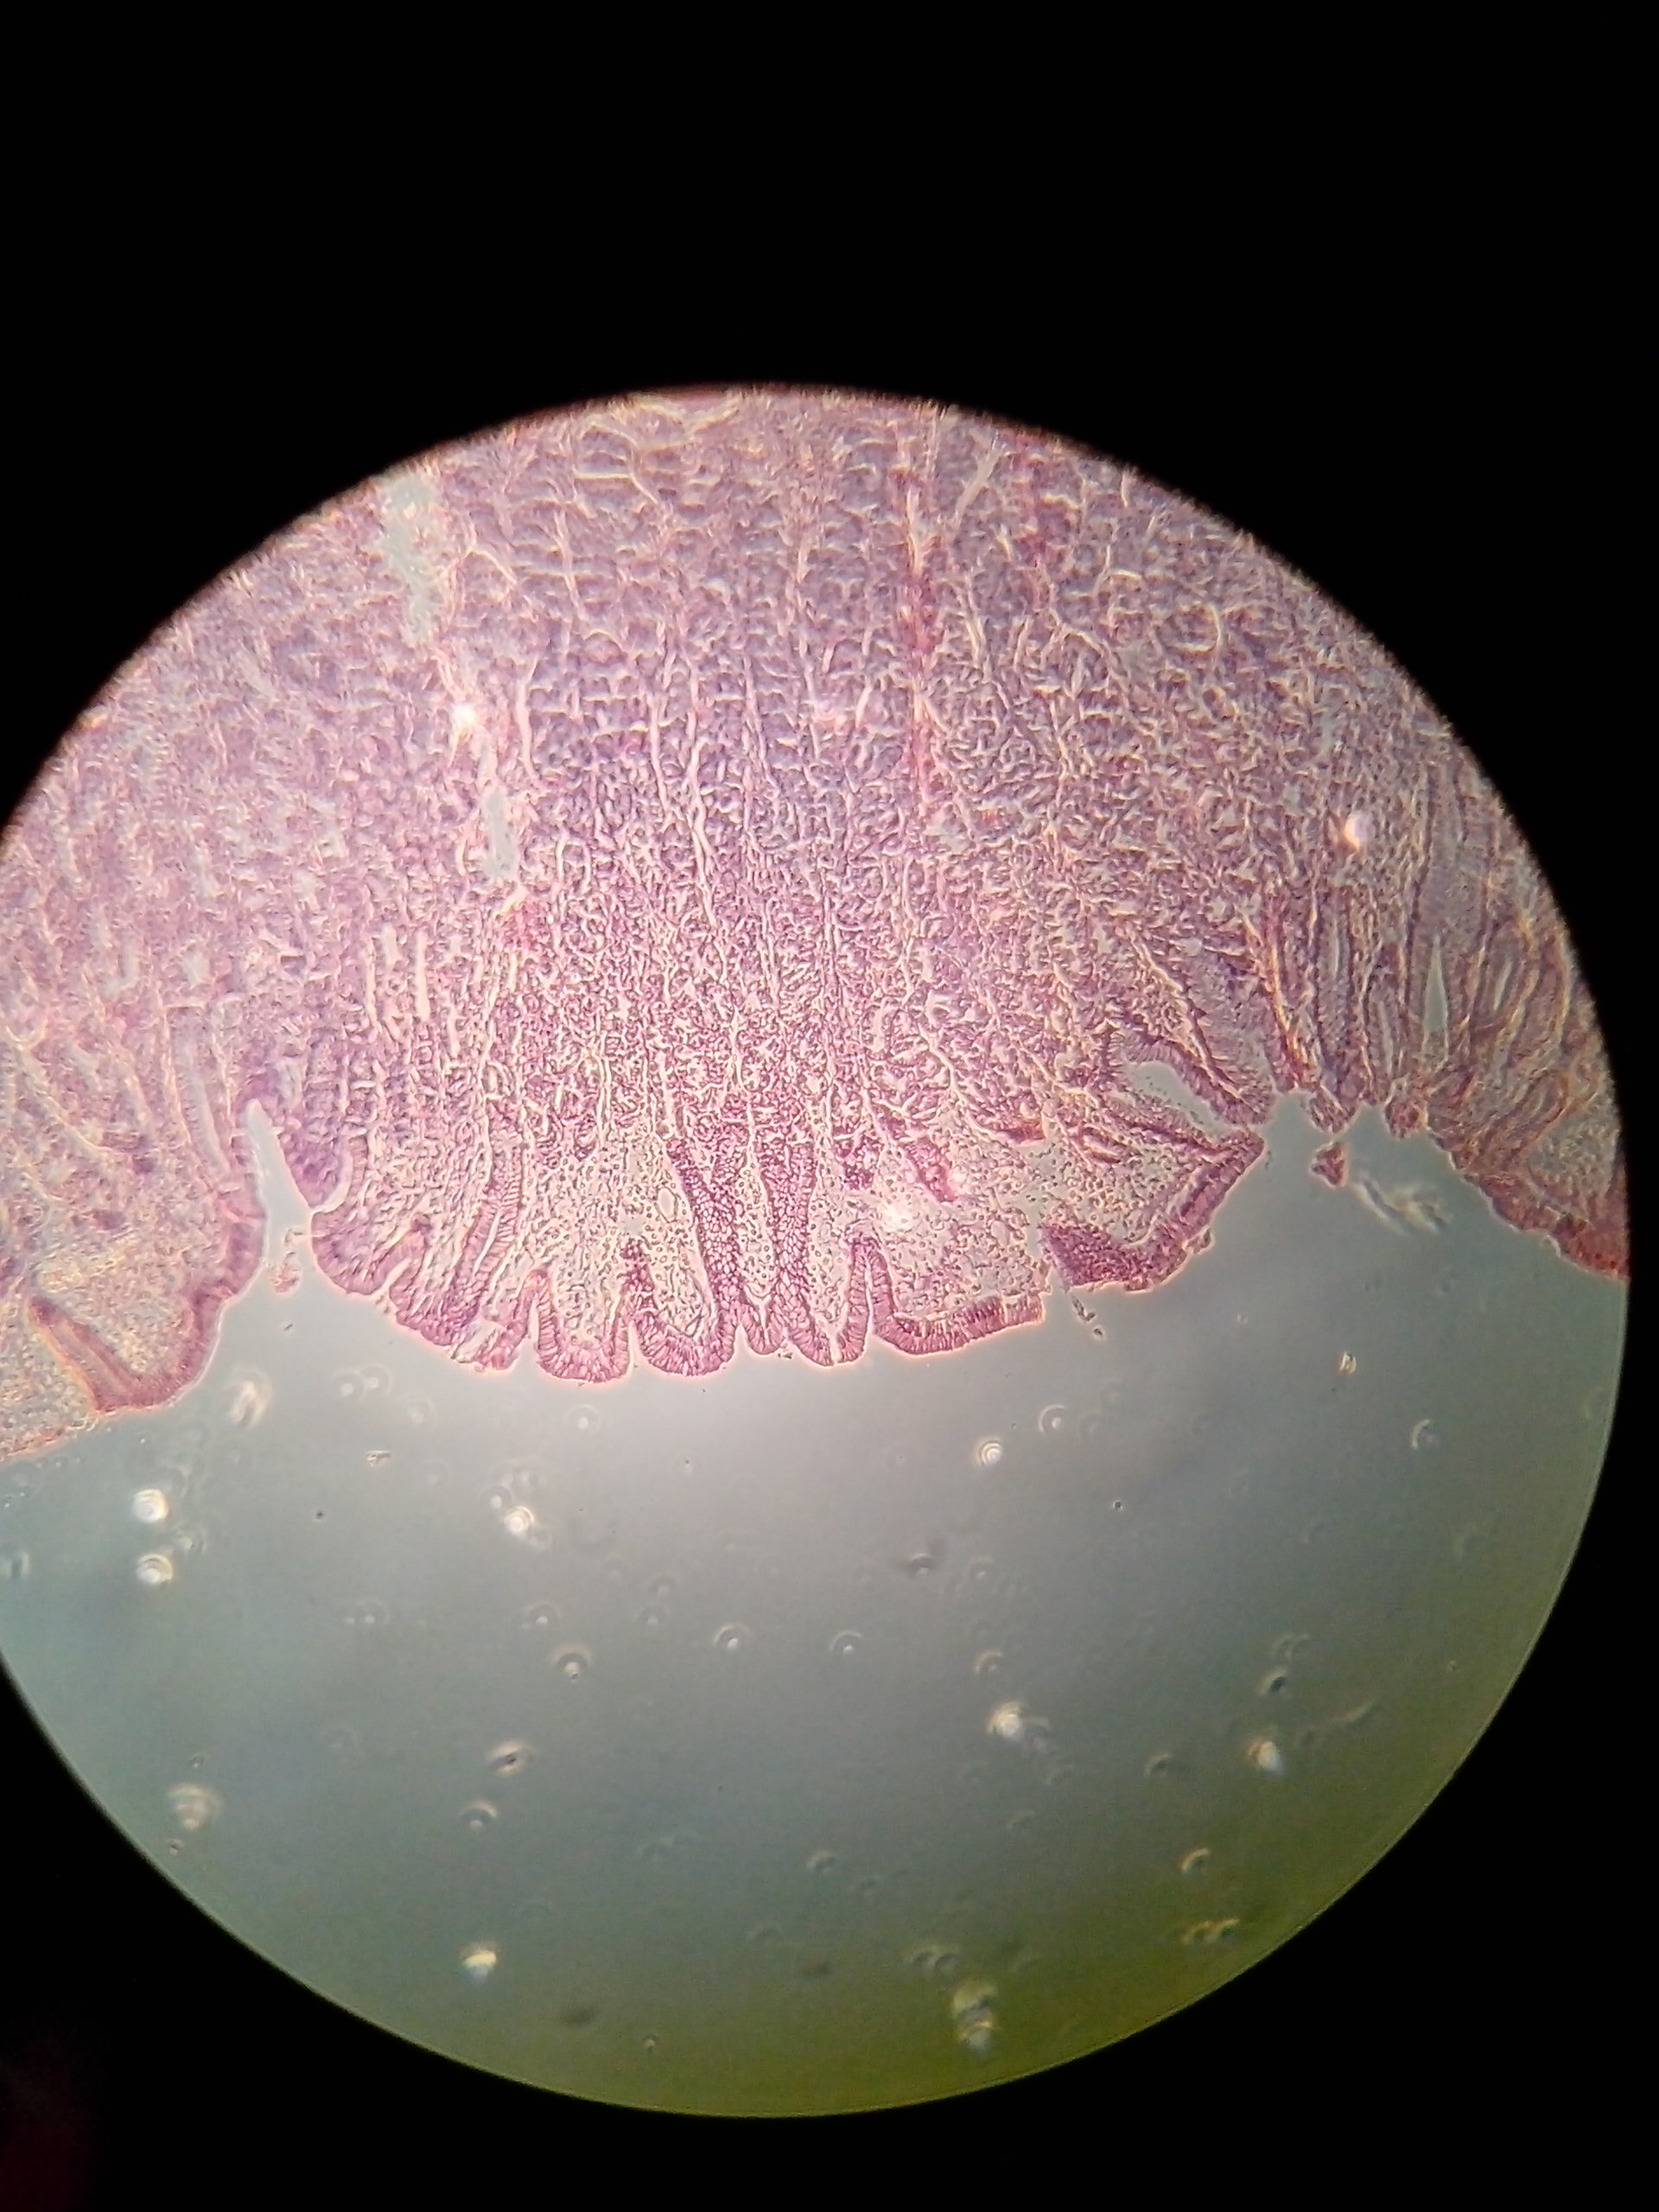
\includegraphics[width=1\textwidth]{../images/02_stomach.jpg}
		\caption{Objektiv 10x}
		\label{fig:02_stomach}
	\end{subfigure}
	\begin{subfigure}[b]{0.3\textwidth}
		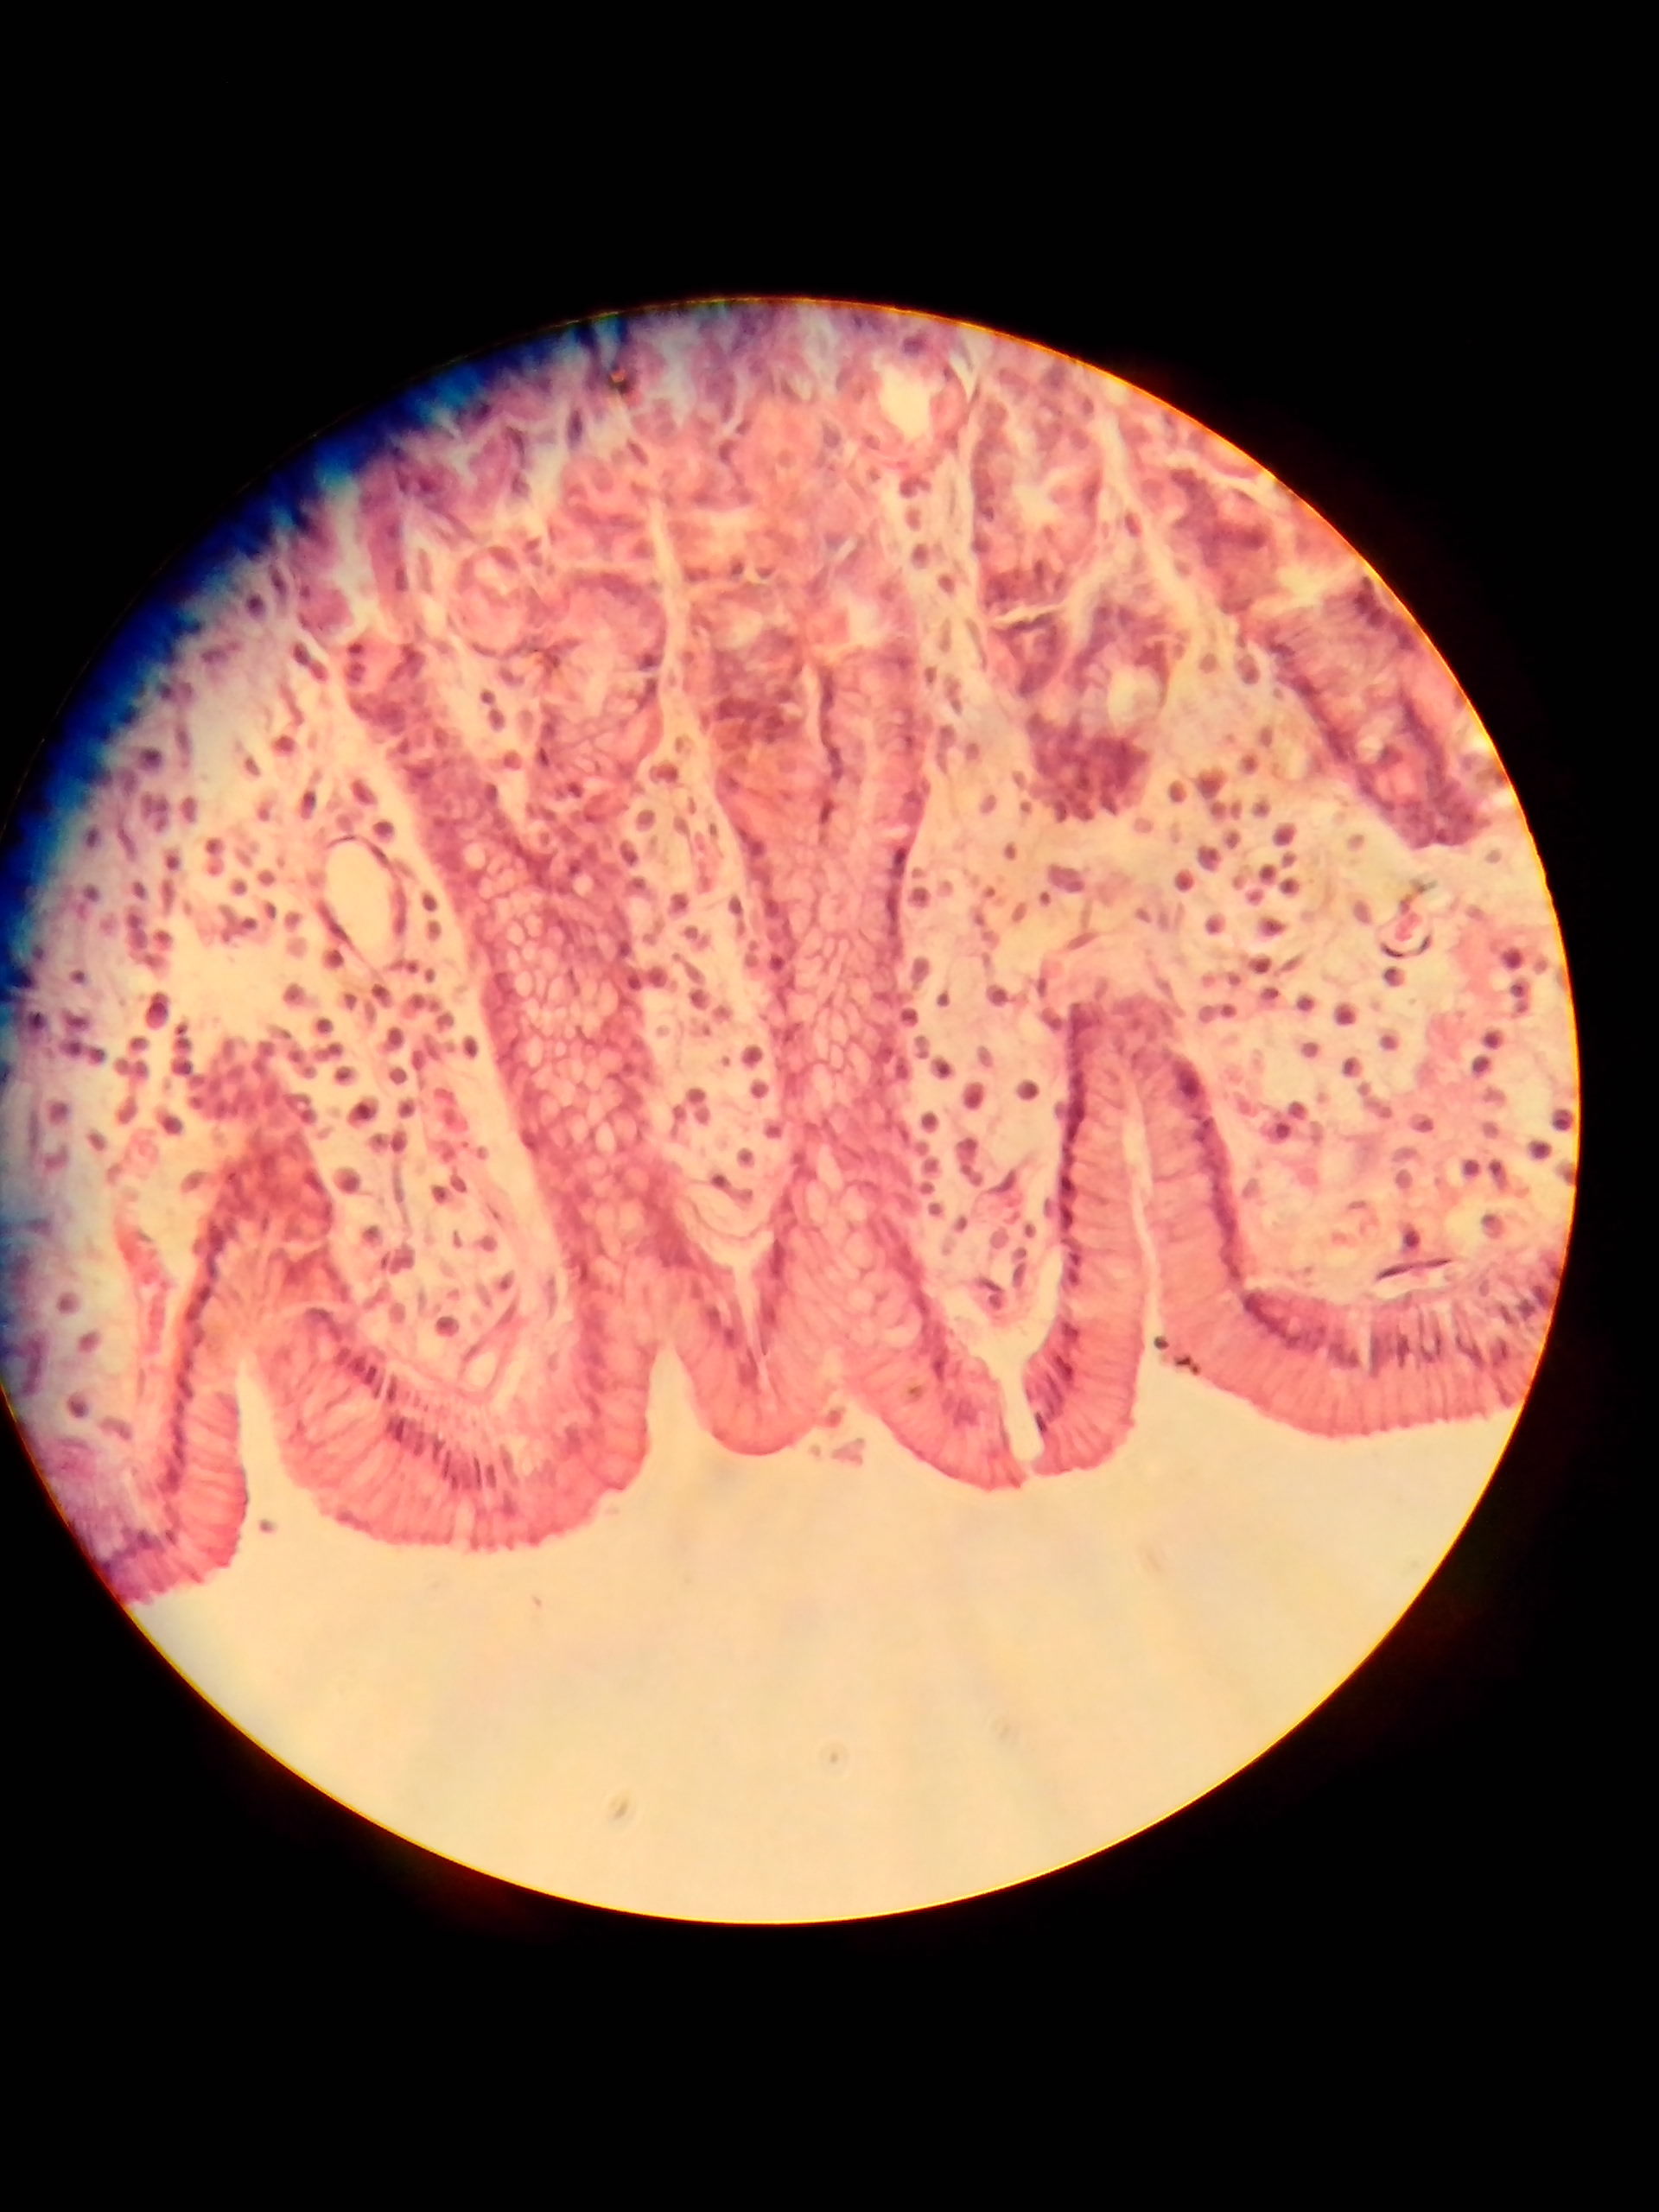
\includegraphics[width=1\textwidth]{../images/03_stomach.jpg}
		\caption{Objektiv 20x}
		\label{fig:03_stomach}
	\end{subfigure}
	\caption{Aufzeichnungen der Lichtmikorskopischen Darstellungen des
		menschlichen Magens}
\end{figure}

\subsubsection{Kommentar}
Der menschliche Magen besteht aus einer Menge an Schichten von verschiedenem
Gewebe. Von besonderer Bedeutung für die Magenfunktion sind die inneren
Schichten des Magens. Hierzu gehört (von Innen nach Aussen) die
Magenschleimhaut, die Bindegewebeschicht und die dahinterliegenden
Muskelschichten (schräg, rund und longitudinal). Die innerste Gewebeschicht
(Magenschleimhaut) mit dem dahinterliegenden Bindegewebe ist in der
Abbildung \ref{fig:01_stomach} zu erkennen. Die Abbildungen
\ref{fig:02_stomach} und \ref{fig:03_stomach} zeigen die erste Gewebeschicht
mit den sogenannten \textit{Foveolae Gastricae} (dt. Magengrübchen) in
höherer Auflösung.

\newpage
\subsection{Menschliche Aorta}

\subsubsection{Proben}
\begin{table}[h!]
	\centering
	\begin{tabular}{l l}
		Bezeichnung	& human aorta \\
		Probe 		& n.a.
	\end{tabular}
\end{table}

\subsubsection{Aufzeichnungen}
\begin{figure}[h!]
	\centering
		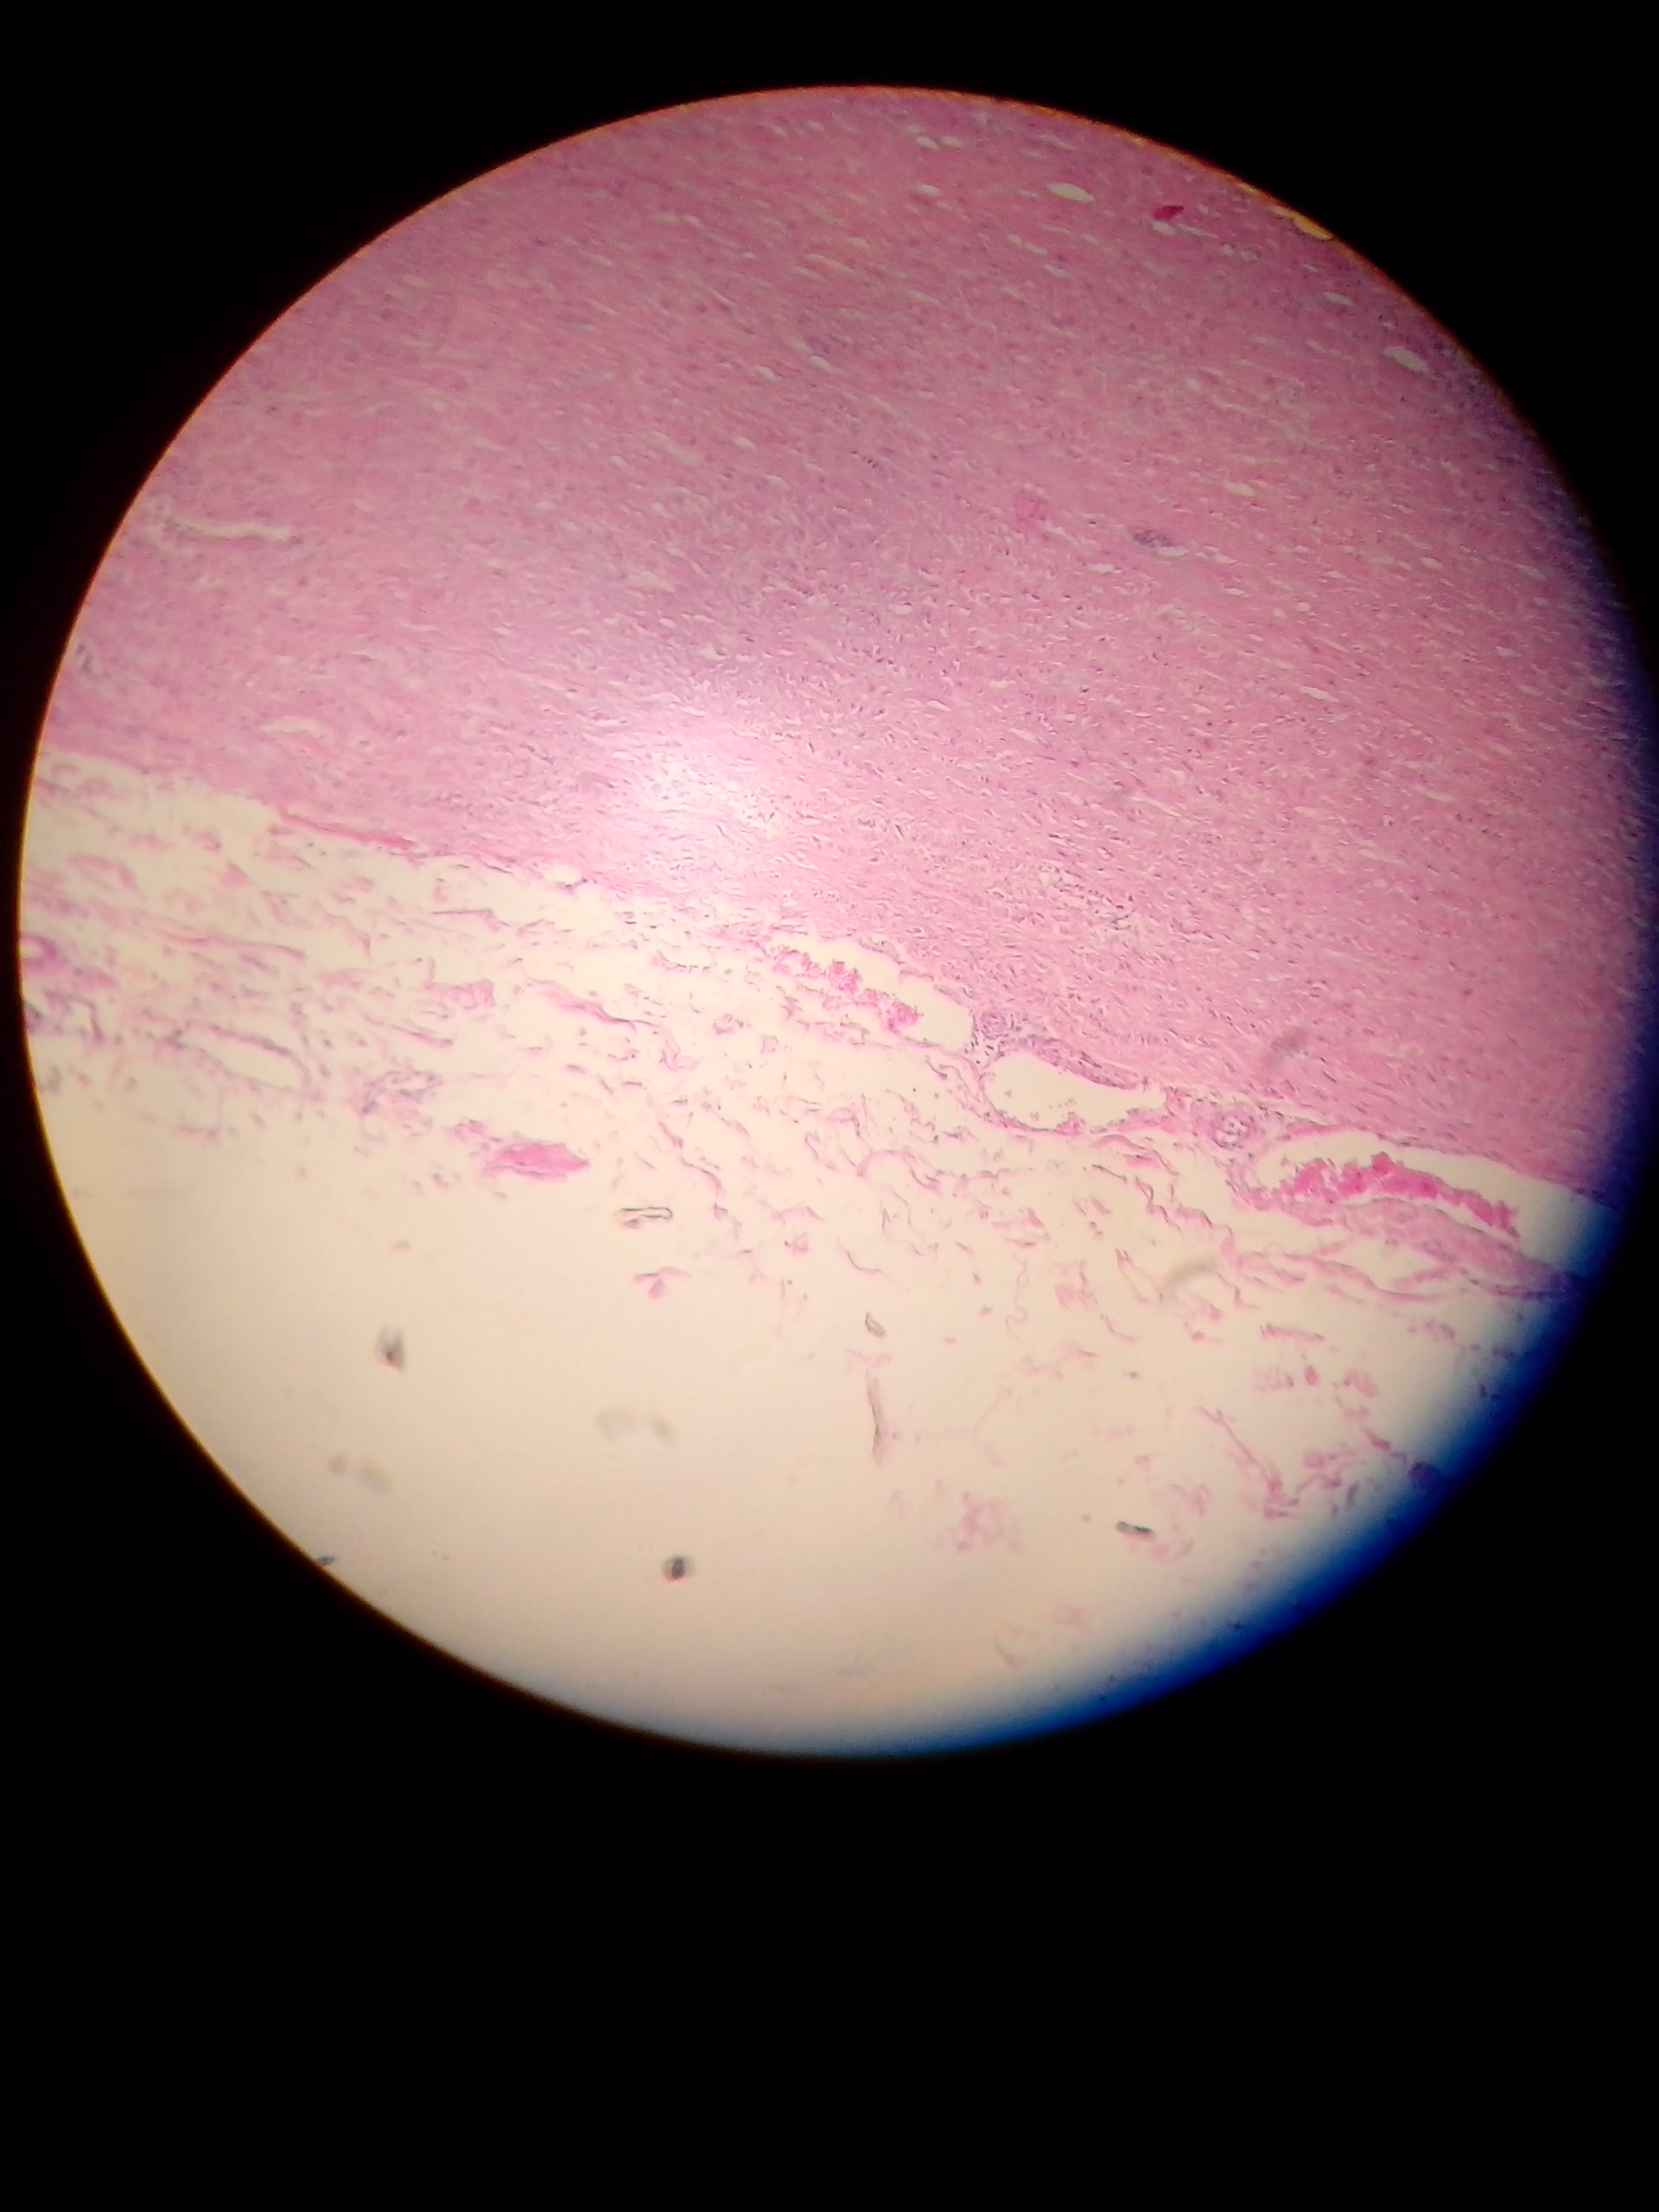
\includegraphics[angle=270, width=0.8\textwidth]{../images/01_aorta.jpg}
		\caption{Objektiv 10x}
	\caption{Aufzeichnungen der Lichtmikorskopischen Darstellungen der
		menschlichen Aorta}
\end{figure}

\subsubsection{Kommentar}

\newpage
\subsection{Blutvergleich von Mensch und Tier}

\subsubsection{Proben}
\begin{table}[h!]
	\centering
	\begin{tabular}{l l l}
		Gegenstand
			& Bezeichnung
			& Probe \\
		\hline
		Vogelblut
			& Bird Blood smear
			& 31-3134 \\
		Froschblut
			& Frog Blood smear
			& 31-3128 \\
		Menschliches Blut
			& Human Blood smear
			& 31-3152 \\
		Eigenes Blut
			& n.a.
			& n.a. \\
	\end{tabular}
\end{table}

\subsubsection{Aufzeichnungen}
\begin{figure}[h!]
	\centering
	\begin{subfigure}[b]{0.3\textwidth}
		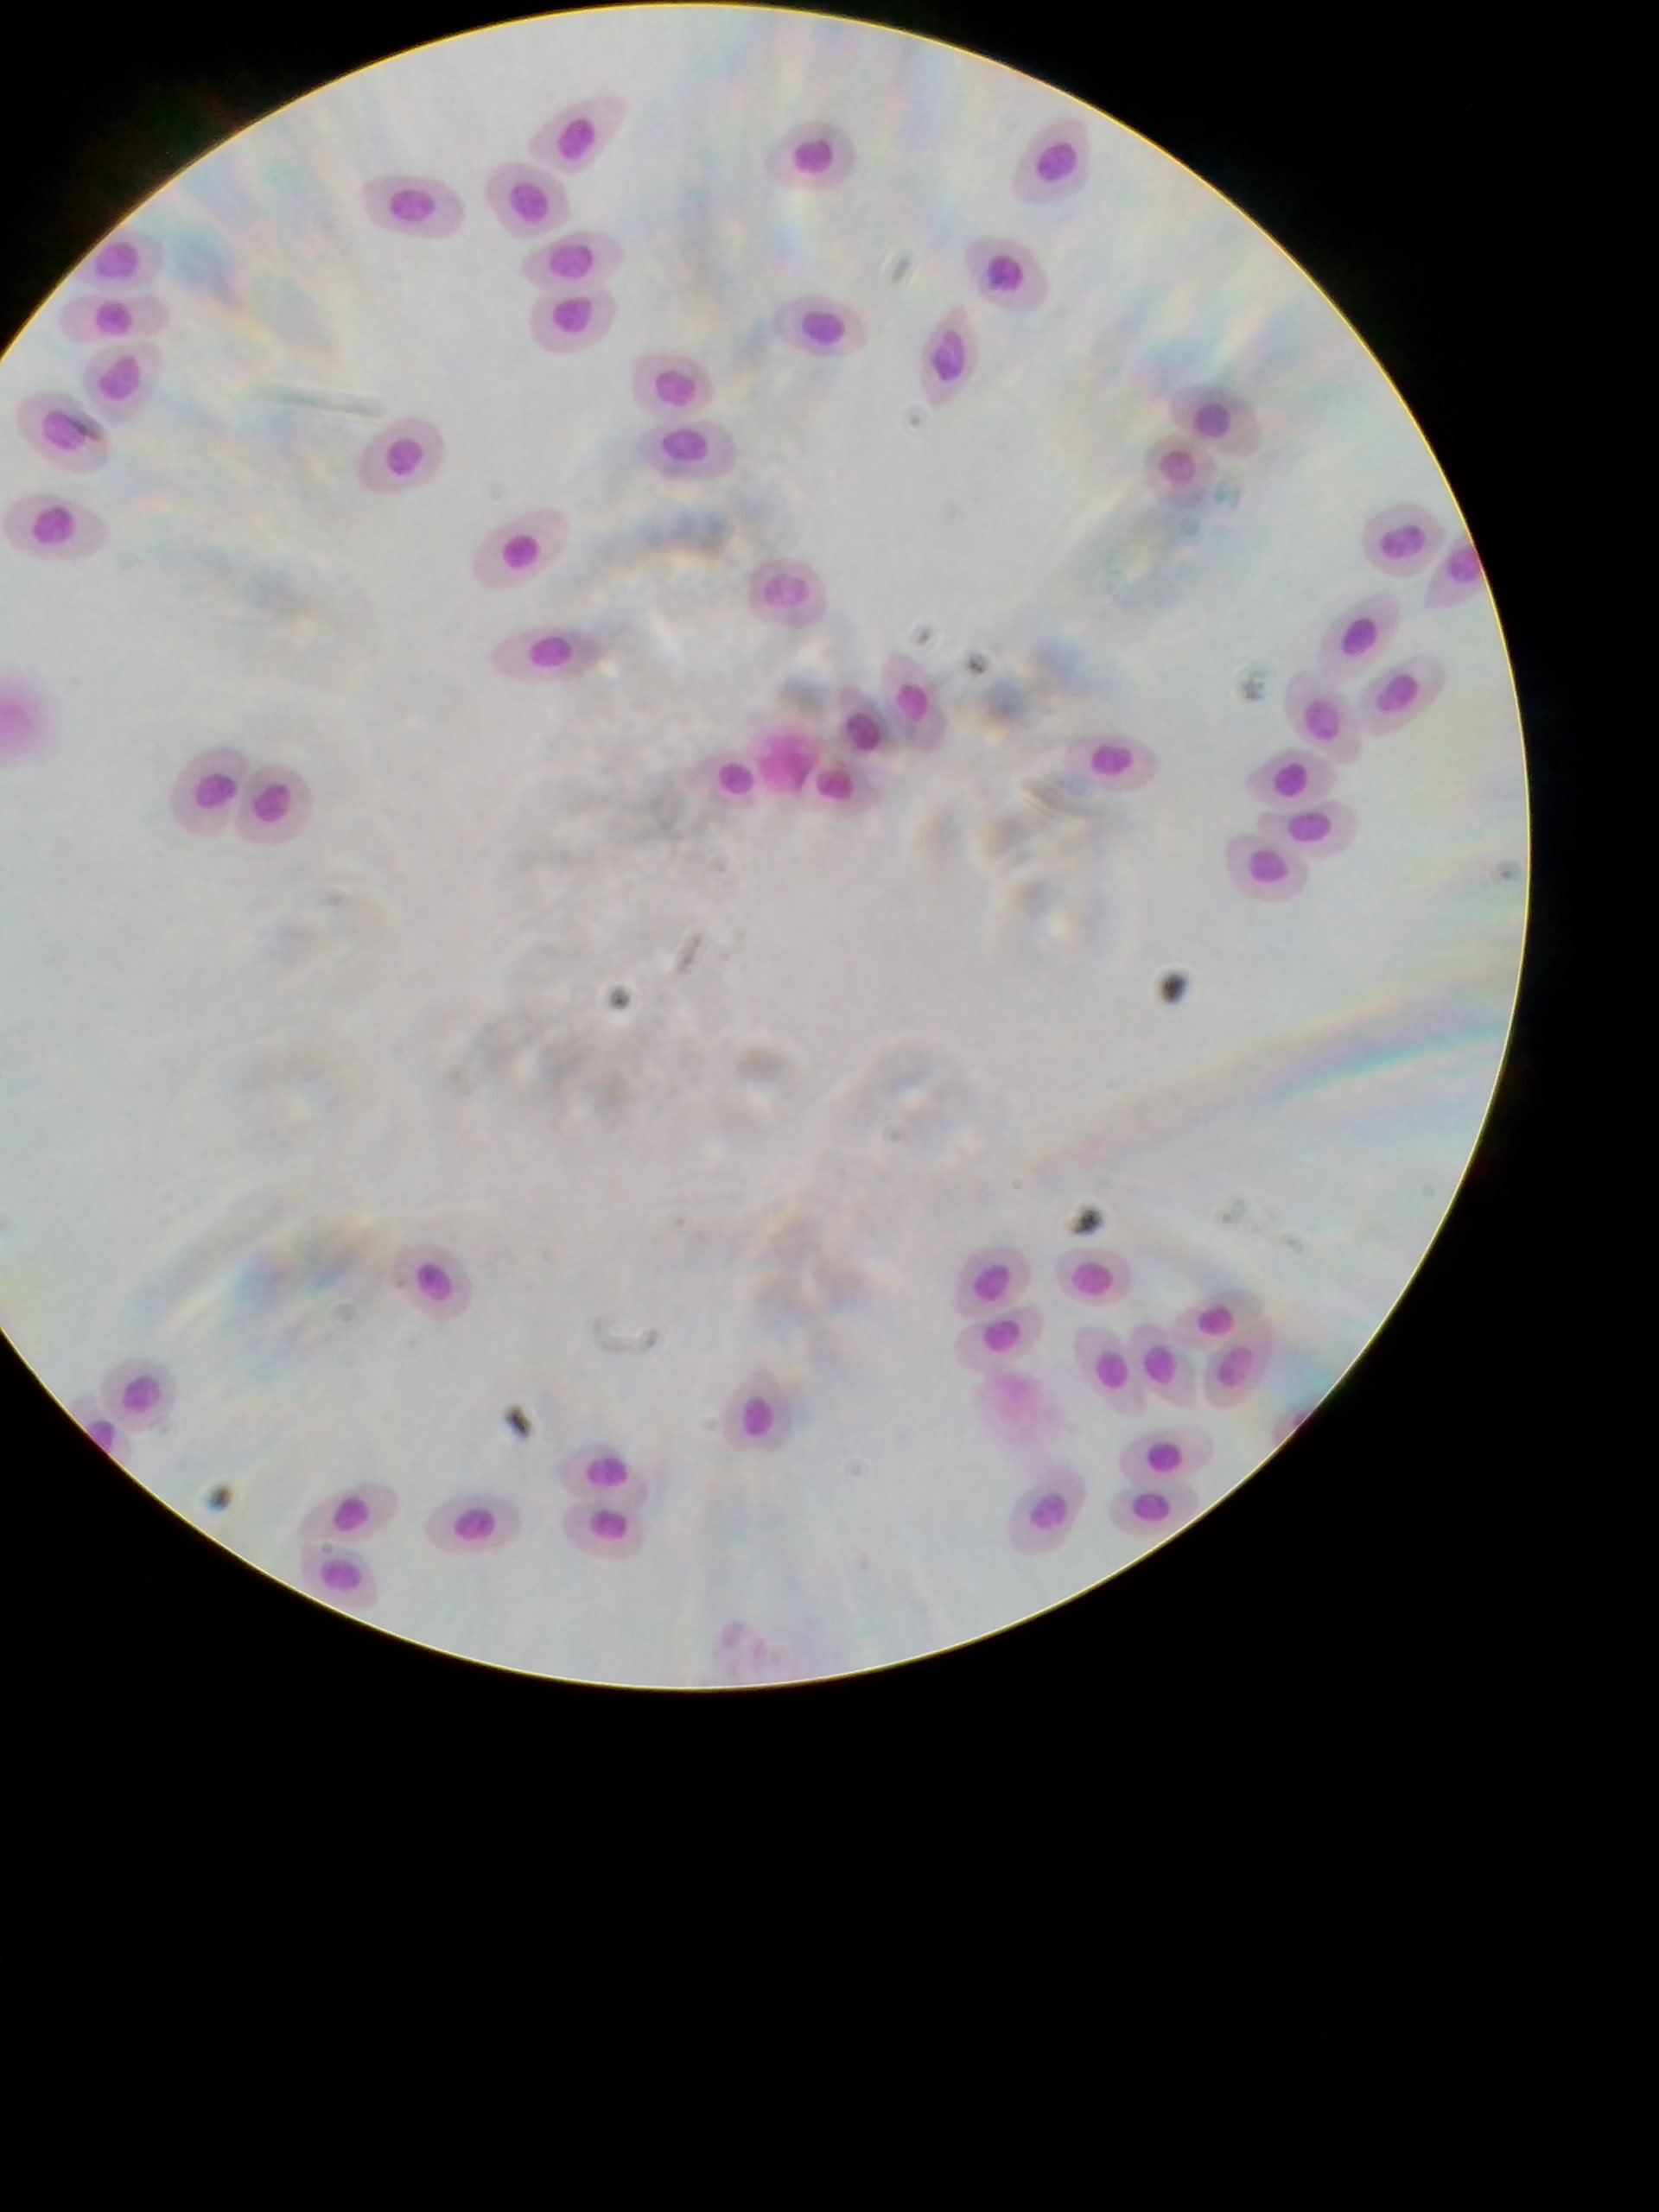
\includegraphics[width=1\textwidth]{../images/02_bird_blood.jpg}
		\caption{Vogelblut -- Objektiv 100x}
	\end{subfigure}
	\begin{subfigure}[b]{0.3\textwidth}
		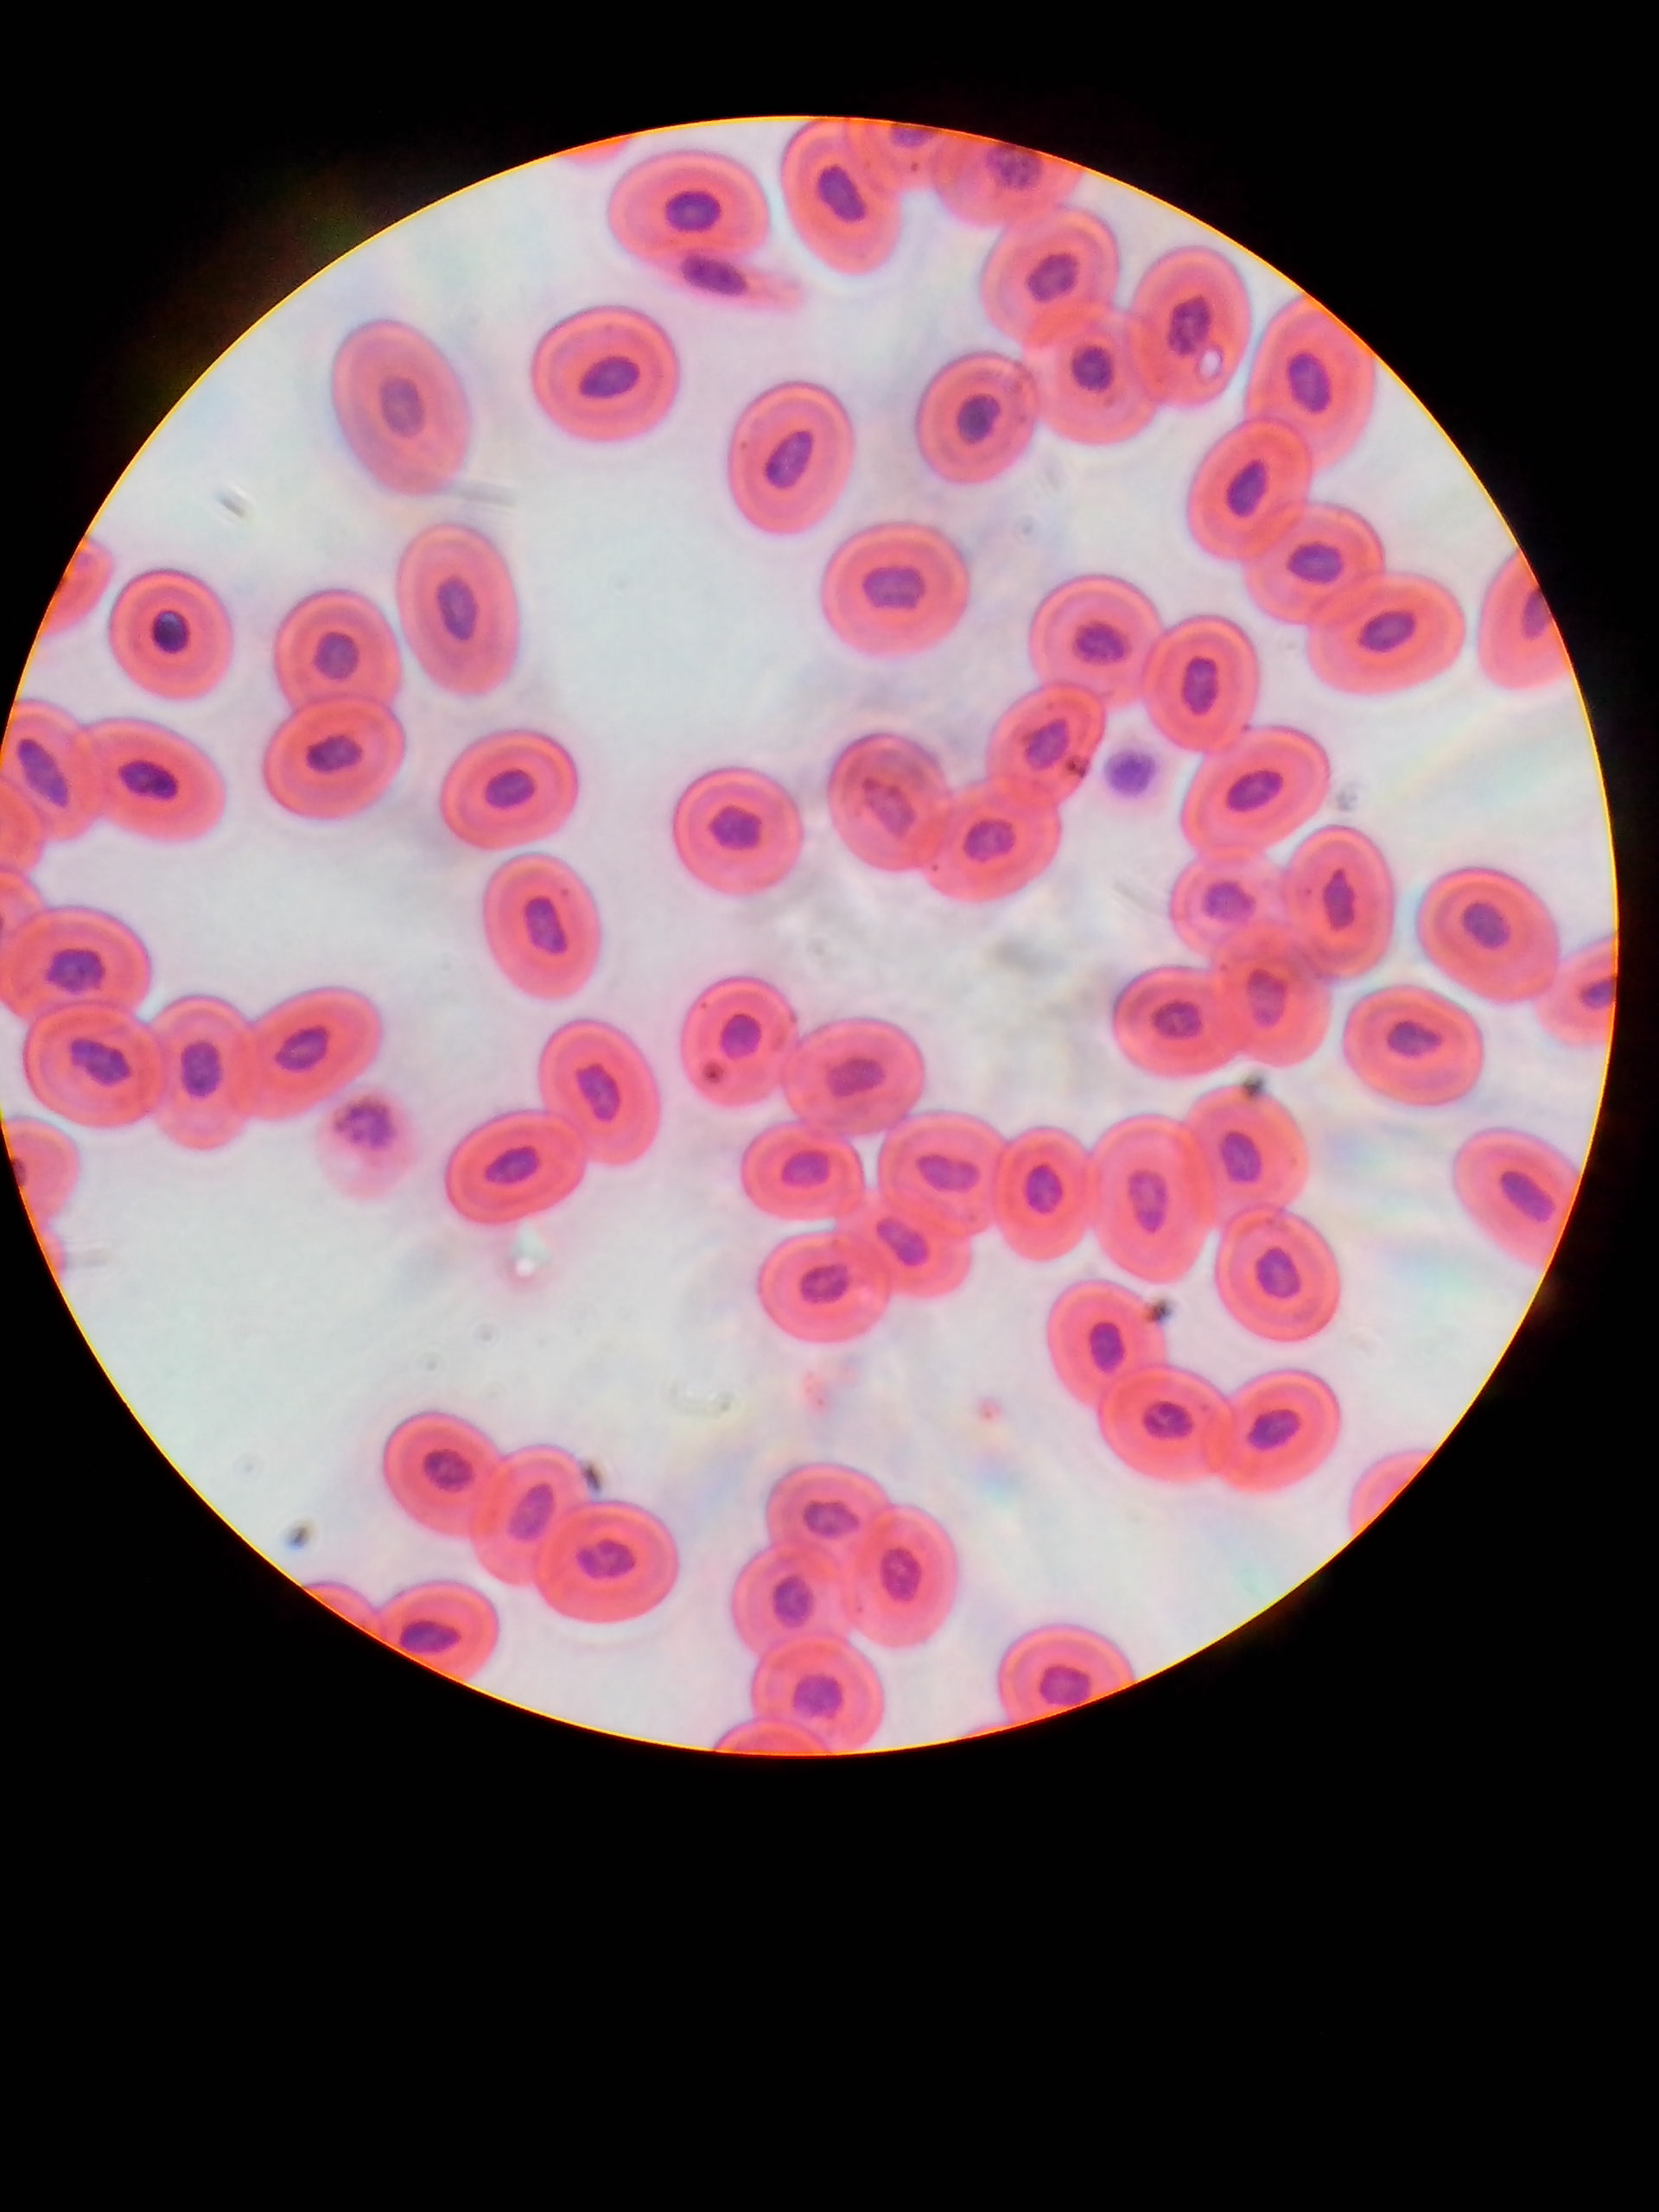
\includegraphics[width=1\textwidth]{../images/01_frog_blood.jpg}
		\caption{Froschblut -- Objektiv 100x}
	\end{subfigure}

	\begin{subfigure}[b]{0.3\textwidth}
		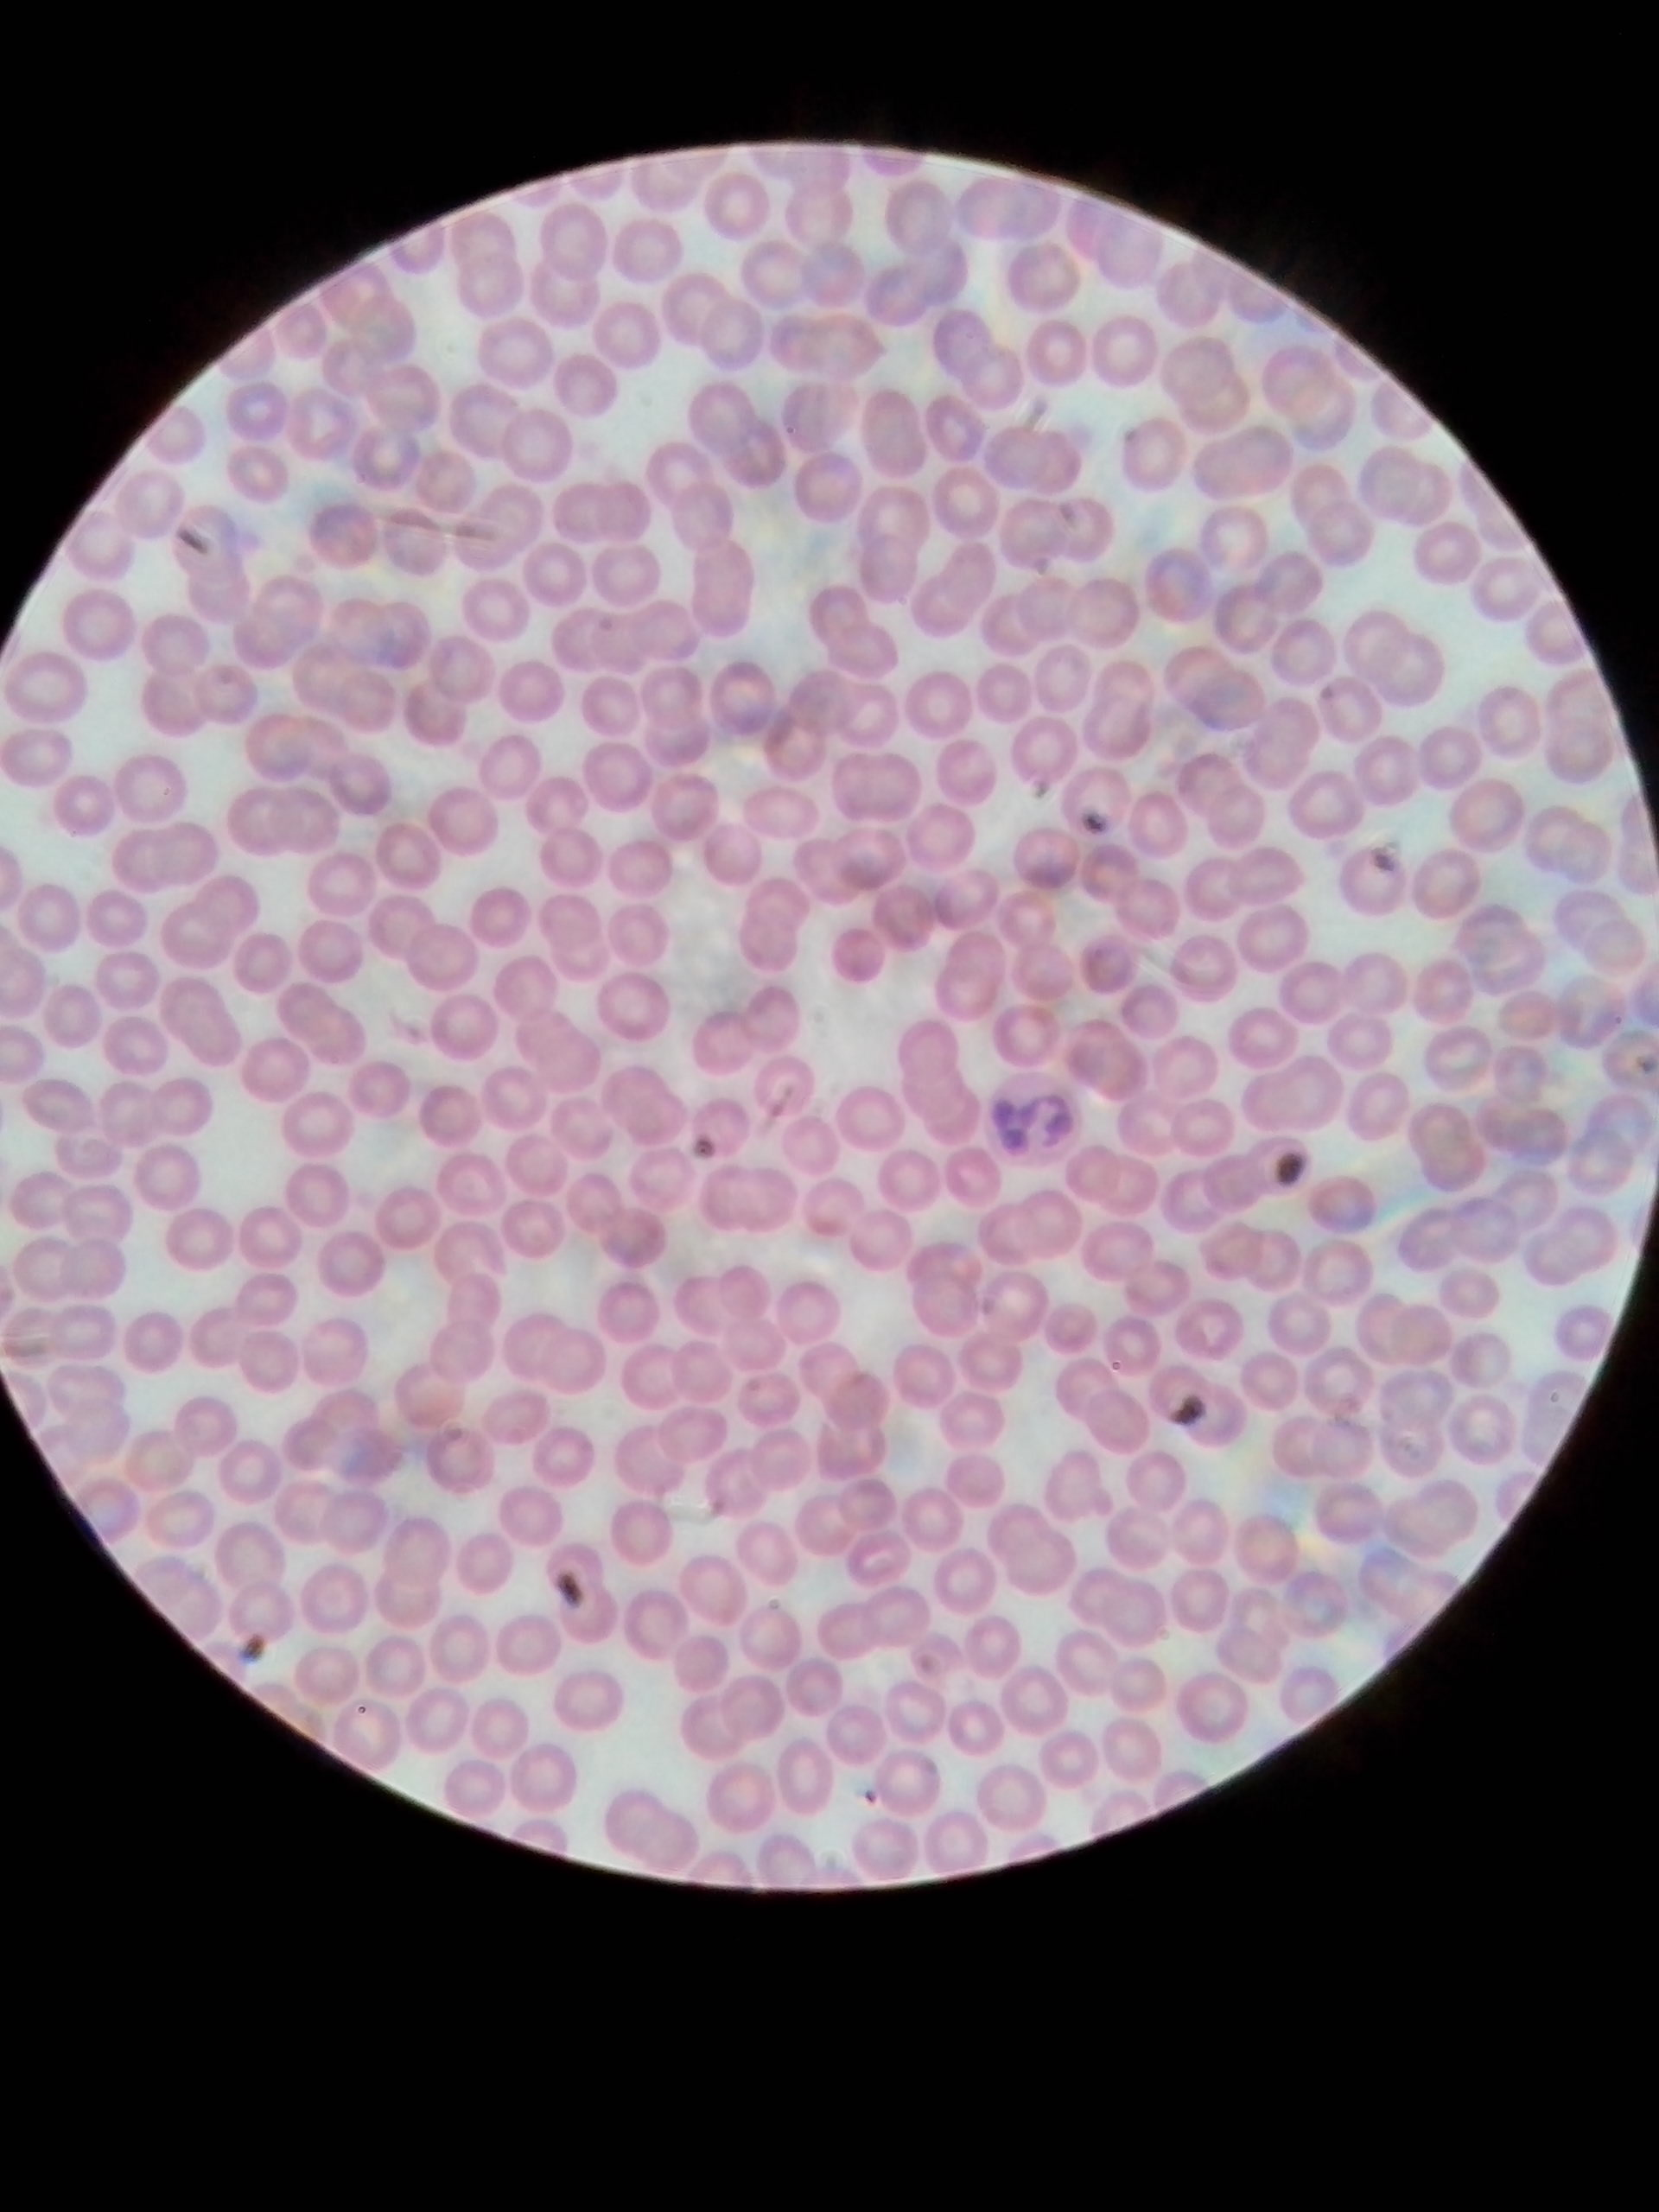
\includegraphics[width=1\textwidth]{../images/01_human_blood.jpg}
		\caption{Menschliches Blut -- Objektiv 100x}
	\end{subfigure}
	\begin{subfigure}[b]{0.3\textwidth}
		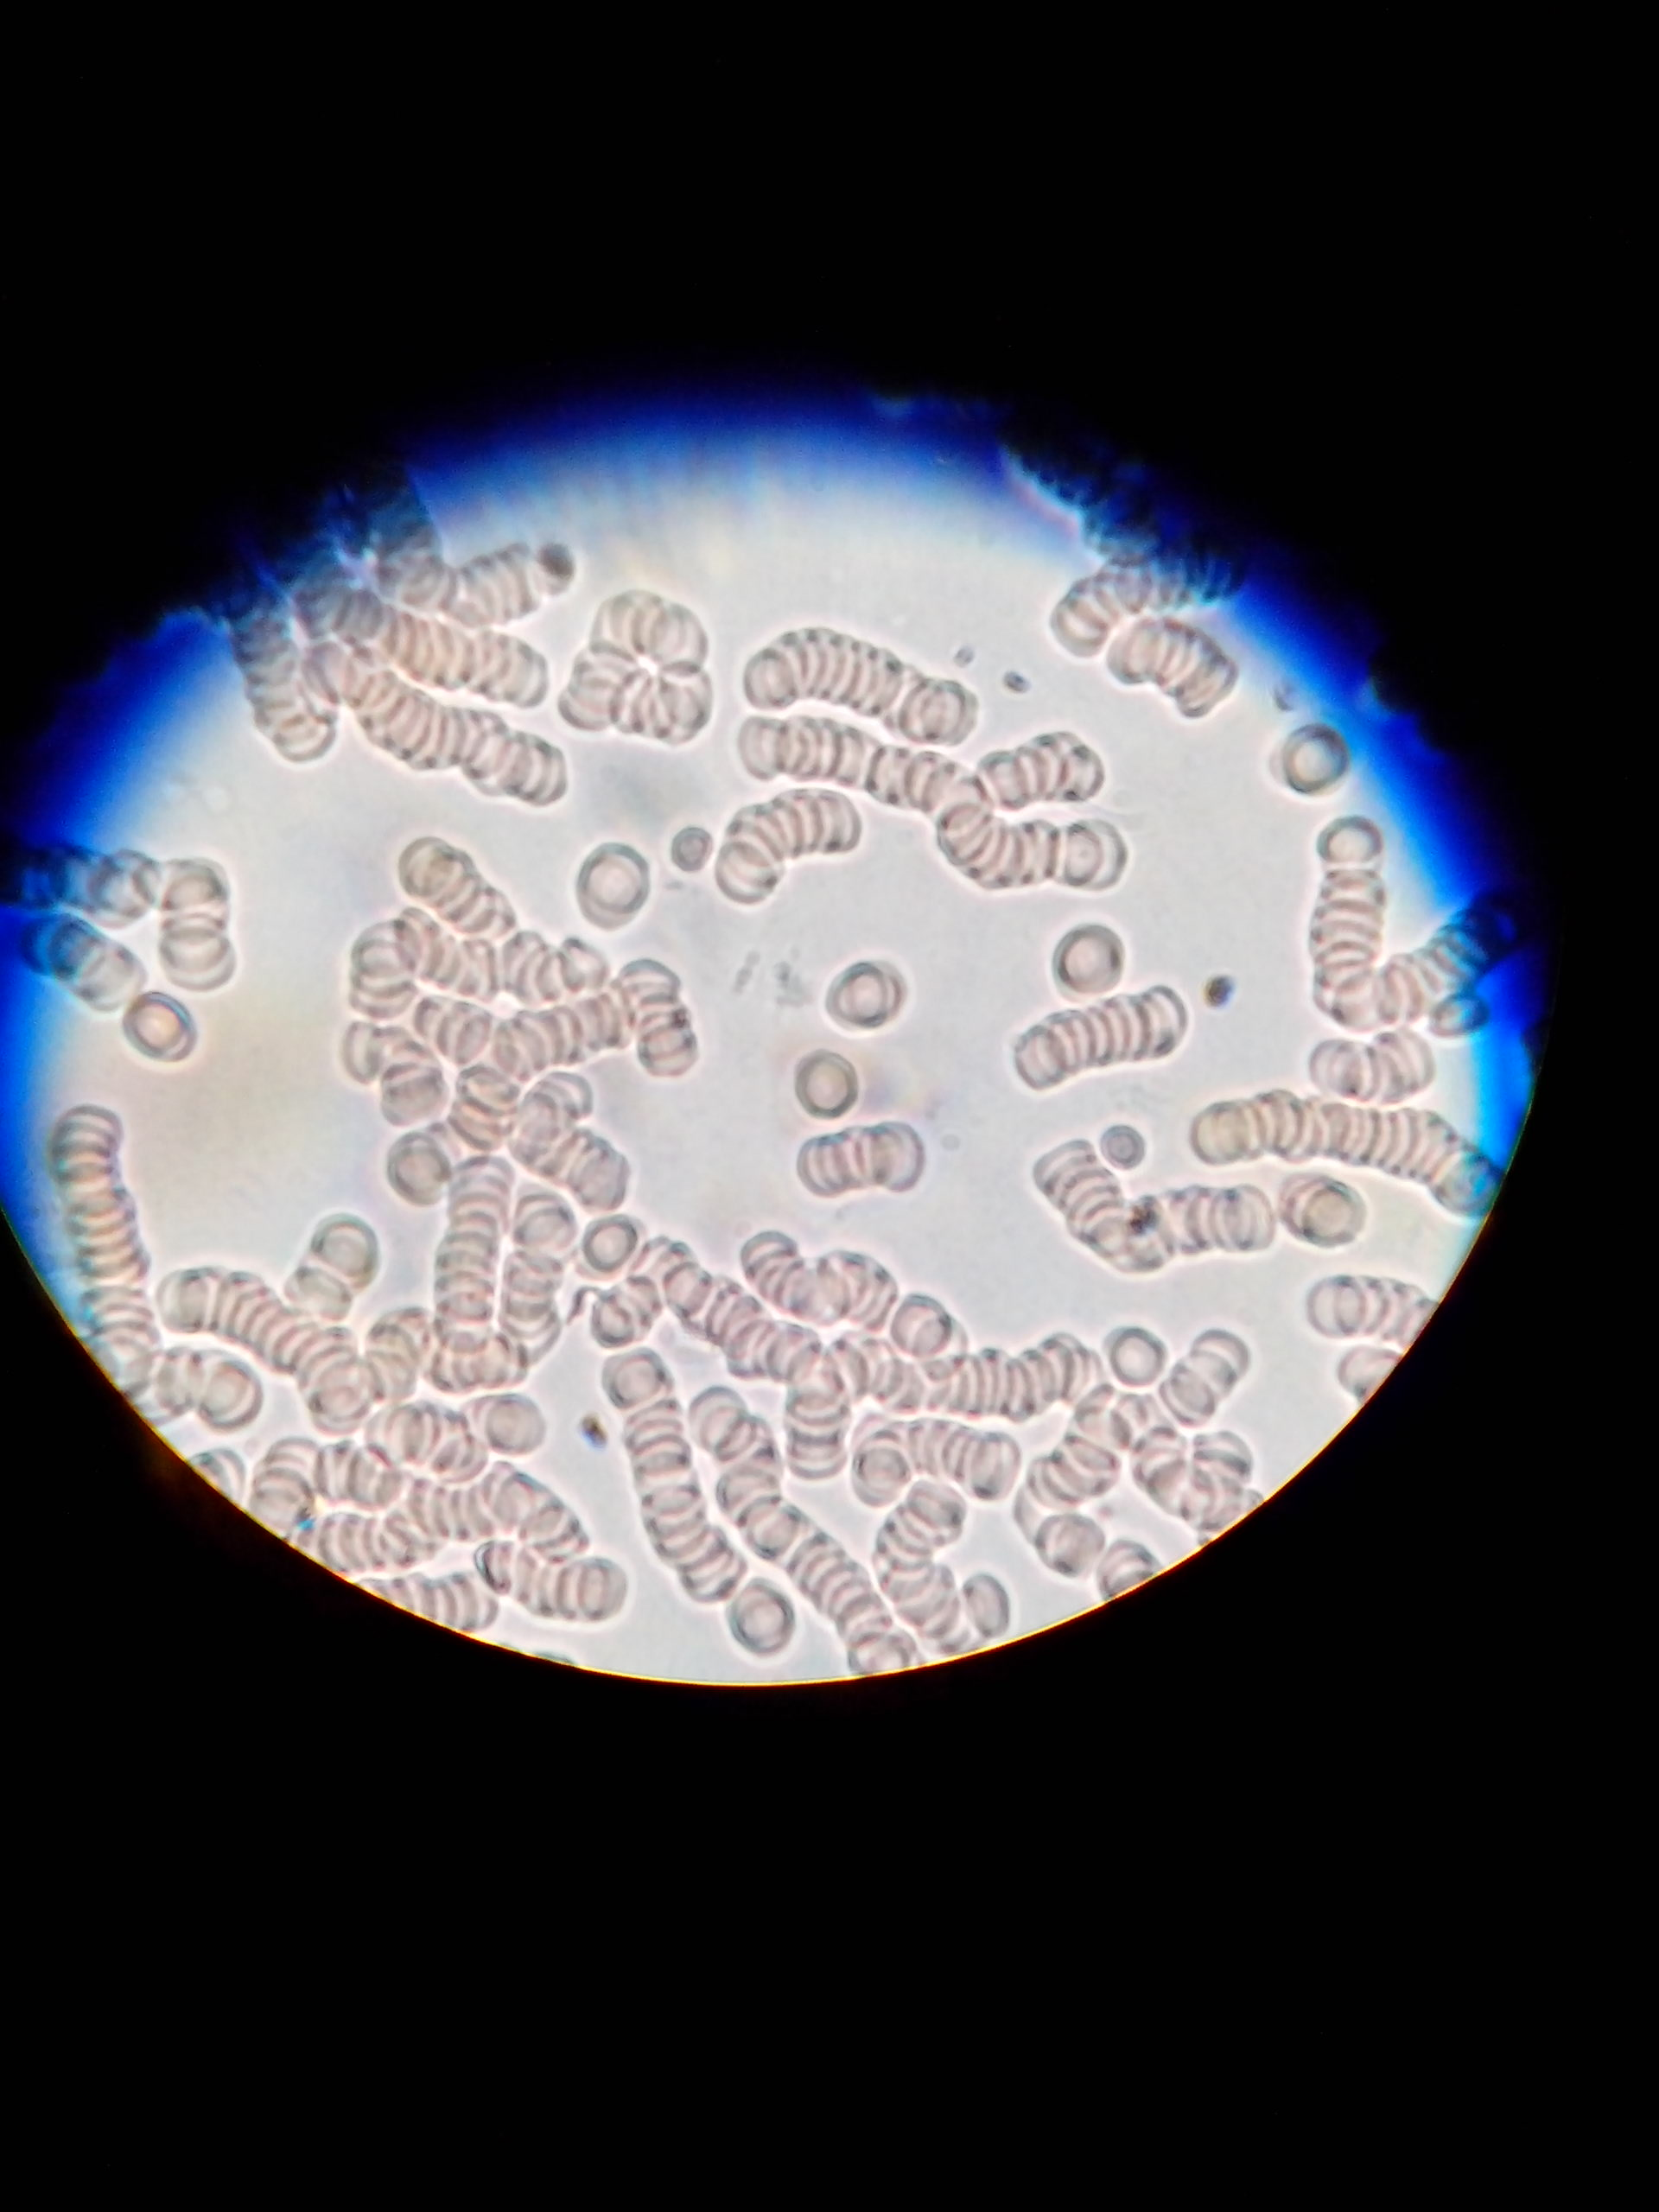
\includegraphics[width=1\textwidth]{../images/02_own_blood.jpg}
		\caption{Menschliches Blut -- Objektiv 100x}
	\end{subfigure}
	\caption{Autzeichnungen der Lichtmikorskopischen Darstellungen der
		verschiedenen Blutproben}
\end{figure}

\subsubsection{Kommentar}
